\documentclass[12pt,a4paper,fleqn]{article}
\usepackage[utf8]{inputenc}
\usepackage[russian]{babel}
\usepackage{amssymb, amsmath, multicol}
\usepackage{enumitem}
\usepackage{lipsum}
\usepackage{euler}
\oddsidemargin=-15.4mm
\textwidth=190mm
\headheight=-32.4mm
\textheight=277mm
\parindent=0pt
\parskip=8pt
\pagestyle{empty}
\usepackage{graphicx}
\title{\textbf{\LARGE{Исследовательская работа по теме:\\Исследование функции дифференциальными методами}}}
\author{Известный гражданин}
\date{November 2022}
\addt\captionsrussian{\def\refname{Список литературы}}\begin{document}
\maketitle
\newpage\newpage \textbf{\LARGE{Глава I. Функция}}

\begin{center}
$y = $$3 \cdot cos(x^{3})$

\end{center}
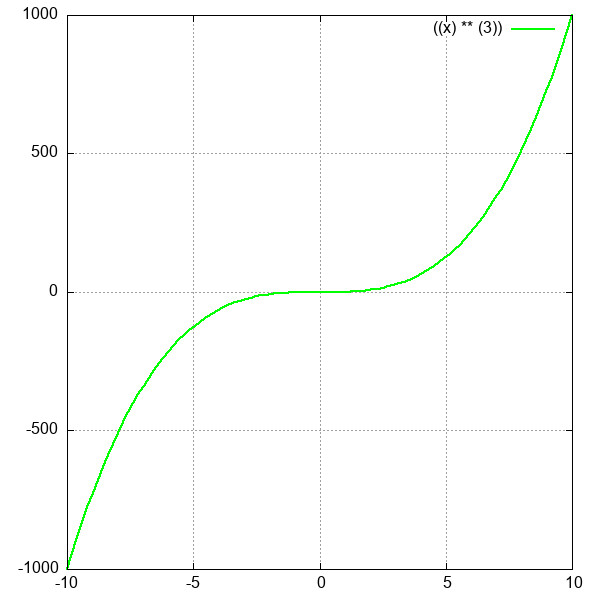
\includegraphics{GraphicDumps/plot.jpg}\newpage \textbf{\LARGE{Глава II. Визуальный анализ функции}}

По теореме Эскобара

\begin{center}
$y = $$3 \cdot cos(x^{3})$

\end{center}
\newpage \textbf{\LARGE{Глава III. Дифференцирование}}

Если вы понимаете данный переход, то я вам сочувствую

\begin{center}
 ($3)'
  = 0$\end{center}
Segmentation fault (core dumped)

\begin{center}
 ($x)'
  = 1$\end{center}
(null)\cite{link4}

\begin{center}
 ($x^{3})'
  = ((3-1) \cdot x^{3-1}) \cdot 1$\end{center}
Segmentation fault (core dumped)

\begin{center}
 ($cos(x^{3}))'
  = (((3-1) \cdot x^{3-1}) \cdot 1) \cdot (0-sin(x^{3}))$\end{center}
//TODO: Лёша, придумай переход. У меня идеи закончились

\begin{center}
A = $(((3-1) \cdot x^{3-1}) \cdot 1) \cdot (0-sin(x^{3}))$\end{center}
\begin{center}
 ($3 \cdot cos(x^{3}))'
  = 0 \cdot cos(x^{3})+3 \cdot (A)$\end{center}
DUMP

$0 \cdot cos(x^{3})+3 \cdot ((((3-1) \cdot x^{3-1}) \cdot 1) \cdot (0-sin(x^{3})))$DUMP
\newpage \textbf{\LARGE{Глава IV.Упрощение выражения}}

Используя выводы из теоремы 1000-7 получаем

\begin{center}$3-1 = 2$\end{center}
Не трудно заметить

\begin{center}$3-1 = 2$\end{center}
Дифференциал Елена всего в 100 метрах от вас...

\begin{center}
$0 \cdot cos(x^{3}) = 0$\end{center}
Руководствуясь базовой логикой, получаем

\begin{center}
$(2 \cdot x^{2}) \cdot 1 = 2 \cdot x^{2}$\end{center}
Руководствуясь сборником <<Задачи для подготовки к поступлению в советские ясли>>\cite{link1}

\begin{center}
$0+3 \cdot ((2 \cdot x^{2}) \cdot (0-sin(x^{3}))) = 3 \cdot ((2 \cdot x^{2}) \cdot (0-sin(x^{3})))$\end{center}
\newpage \textbf{\LARGE{Глава V. Полученая производная}}

$y = $$3 \cdot cos(x^{3})$

$y' = $$3 \cdot ((2 \cdot x^{2}) \cdot (0-sin(x^{3})))$

\includegraphics{GraphicDumps/plot_1.jpg}\newpage \textbf{\LARGE{Глава VI. Разложение функции по формуле Тейлора}}

При этом

\begin{center}$0^{3} = 0$\end{center}
Первая производная комом\cite{link2}

\begin{center}$cos(0) = 1$\end{center}
Нам не объяснили на семинаре как это делать, поэтому примем на веру

\begin{center}$3 \cdot 1 = 3$\end{center}
Если вы понимаете данный переход, то я вам сочувствую

\begin{center}
 ($3)'
  = 0$\end{center}
//TODO: Лёша, придумай переход. У меня идеи закончились

\begin{center}
 ($x)'
  = 1$\end{center}
Так как 1=1, то\cite{link4}

\begin{center}
 ($x^{3})'
  = ((3-1) \cdot x^{3-1}) \cdot 1$\end{center}
Используя выводы из теоремы 1000-7 получаем

\begin{center}
 ($cos(x^{3}))'
  = (((3-1) \cdot x^{3-1}) \cdot 1) \cdot (0-sin(x^{3}))$\end{center}
Как будет доказано в следующем семестре

\begin{center}
A = $(((3-1) \cdot x^{3-1}) \cdot 1) \cdot (0-sin(x^{3}))$\end{center}
\begin{center}
 ($3 \cdot cos(x^{3}))'
  = 0 \cdot cos(x^{3})+3 \cdot (A)$\end{center}
Единственное, что я не понимаю, так это то, зачем ты это читаешь

\begin{center}$3-1 = 2$\end{center}
//TODO: Лёша, придумай переход. У меня идеи закончились

\begin{center}$3-1 = 2$\end{center}
Телец в козероге, поэтому

\begin{center}
$0 \cdot cos(x^{3}) = 0$\end{center}
Доказательство данного факта предоставлено лицом или организацией исполняющей функции иностанного агента

\begin{center}
$(2 \cdot x^{2}) \cdot 1 = 2 \cdot x^{2}$\end{center}
Если посмотреть на выражение под другим углом, можно получить

\begin{center}
$0+3 \cdot ((2 \cdot x^{2}) \cdot (0-sin(x^{3}))) = 3 \cdot ((2 \cdot x^{2}) \cdot (0-sin(x^{3})))$\end{center}
Руководствуясь базовой логикой, получаем

\begin{center}$0^{2} = 0$\end{center}
Поэтому

\begin{center}$2 \cdot 0 = 0$\end{center}
Дураку понятно, что

\begin{center}$0^{3} = 0$\end{center}
Доказательство данного факта предоставлено лицом или организацией исполняющей функции иностанного агента

\begin{center}$sin(0) = 0$\end{center}
Только 0.00001 процент умнейших людей планеты смогут понять этот переход

\begin{center}$0-0 = 0$\end{center}
Очевидно, что

\begin{center}$0 \cdot 0 = 0$\end{center}
Segmentation fault (core dumped)

\begin{center}$3 \cdot 0 = 0$\end{center}
Руководствуясь сборником <<Задачи для подготовки к поступлению в советские ясли>>\cite{link1}

\begin{center}$\frac{0}{1} = 0$\end{center}
Руководствуясь базовой логикой, получаем

\begin{center}
$x-0 = x$\end{center}
А теперь уберите детей от экранов

\begin{center}
$x^{1} = x$\end{center}
Единственное, что я не понимаю, так это то, зачем ты это читаешь

\begin{center}
$0 \cdot x = 0$\end{center}
При этом

\begin{center}
 ($3)'
  = 0$\end{center}
Хорошо там, где производной нет\cite{link2}

\begin{center}
 ($2)'
  = 0$\end{center}
Дефии... кхм, Дифири... тьфу ты, дифферин... Да что ж со мной такое сегодня? Дифференциал. Уф, совсем я заработался. Пойду отдохну *звук отодвигаемого стула, затем удаляющихся шагов*

\begin{center}
 ($x)'
  = 1$\end{center}
Очевидно, что

\begin{center}
 ($x^{2})'
  = ((2-1) \cdot x^{2-1}) \cdot 1$\end{center}
Руководствуясь базовой логикой, получаем

\begin{center}
 ($2 \cdot x^{2})'
  = 0 \cdot x^{2}+2 \cdot (((2-1) \cdot x^{2-1}) \cdot 1)$\end{center}
По лемме $\sqrt{-759}$
\begin{center}
 ($0)'
  = 0$\end{center}
Нам не объяснили на семинаре как это делать, поэтому примем на веру

\begin{center}
 ($x)'
  = 1$\end{center}
По лемме $\sqrt{-759}$
\begin{center}
 ($x^{3})'
  = ((3-1) \cdot x^{3-1}) \cdot 1$\end{center}
Как будет доказано в следующем семестре

\begin{center}
 ($sin(x^{3}))'
  = (((3-1) \cdot x^{3-1}) \cdot 1) \cdot cos(x^{3})$\end{center}
Не трудно заметить

\begin{center}
A = $(((3-1) \cdot x^{3-1}) \cdot 1) \cdot cos(x^{3})$\end{center}
\begin{center}
 ($0-sin(x^{3}))'
  = 0-A$\end{center}
Здесь могла быть ваша реклама

\begin{center}
A = $0 \cdot x^{2}+2 \cdot (((2-1) \cdot x^{2-1}) \cdot 1)$\end{center}
\begin{center}
B = $(((3-1) \cdot x^{3-1}) \cdot 1) \cdot cos(x^{3})$\end{center}
\begin{center}
 ($(2 \cdot x^{2}) \cdot (0-sin(x^{3})))'
  = (A) \cdot (0-sin(x^{3}))+(2 \cdot x^{2}) \cdot (0-B)$\end{center}
Как было показано ранее

\begin{center}
A = $0 \cdot x^{2}+2 \cdot (((2-1) \cdot x^{2-1}) \cdot 1)$\end{center}
\begin{center}
B = $(((3-1) \cdot x^{3-1}) \cdot 1) \cdot cos(x^{3})$\end{center}
\begin{center}
 ($3 \cdot ((2 \cdot x^{2}) \cdot (0-sin(x^{3}))))'
  = 0 \cdot ((2 \cdot x^{2}) \cdot (0-sin(x^{3})))+3 \cdot ((A) \cdot (0-sin(x^{3}))+(2 \cdot x^{2}) \cdot (0-B))$\end{center}
С другой стороны

\begin{center}$2-1 = 1$\end{center}
Дифференциал от производной не далеко падает\cite{link2}

\begin{center}$2-1 = 1$\end{center}
Говорят

\begin{center}$3-1 = 2$\end{center}
ИИИИЕЕЕЕсли\cite{link3}

\begin{center}$3-1 = 2$\end{center}
Британские учёные доказали, что для поддержания мозга в тонусе необходимо ежедневно дифференцировать. Продолжим наше приобщение к здоровому образу жизниn

\begin{center}
$0 \cdot ((2 \cdot x^{2}) \cdot (0-sin(x^{3}))) = 0$\end{center}
Спешка нужна только в армии и при ловле блох. Но не как уж ни при вычислении производной\cite{link2}

\begin{center}
$0 \cdot x^{2} = 0$\end{center}
Для любого эпсилон больше нулю очевидно, что

\begin{center}
$x^{1} = x$\end{center}
И хотя клуб любителей таких формул двумя блоками ниже, мы продолжаем

\begin{center}
$1 \cdot x = x$\end{center}
С другой стороны

\begin{center}
$x \cdot 1 = x$\end{center}
Британские учёные доказали, что для поддержания мозга в тонусе необходимо ежедневно дифференцировать. Продолжим наше приобщение к здоровому образу жизниn

\begin{center}
$0+2 \cdot x = 2 \cdot x$\end{center}
Первая производная комом\cite{link2}

\begin{center}
$(2 \cdot x^{2}) \cdot 1 = 2 \cdot x^{2}$\end{center}
Обоснование этого пререхода предостовляется читателю в платном DLC

\begin{center}
A = $(2 \cdot x^{2}) \cdot (0-(2 \cdot x^{2}) \cdot cos(x^{3}))$\end{center}
\begin{center}
$0+3 \cdot ((2 \cdot x) \cdot (0-sin(x^{3}))+A) = 3 \cdot ((2 \cdot x) \cdot (0-sin(x^{3}))+A)$\end{center}
Функция производной не стоит\cite{link2}

\begin{center}$2 \cdot 0 = 0$\end{center}
Если посмотреть на выражение под другим углом, можно получить

\begin{center}$0^{3} = 0$\end{center}
И хотя клуб любителей таких формул двумя блоками ниже, мы продолжаем

\begin{center}$sin(0) = 0$\end{center}
Спешка нужна только в армии и при ловле блох. Но не как уж ни при вычислении производной\cite{link2}

\begin{center}$0-0 = 0$\end{center}
Без комментариев\cite{link4}

\begin{center}$0 \cdot 0 = 0$\end{center}
Положим

\begin{center}$0^{2} = 0$\end{center}
Автору приснилось, что следующее преобразование верно

\begin{center}$2 \cdot 0 = 0$\end{center}
Функция производной не стоит\cite{link2}

\begin{center}$0^{2} = 0$\end{center}
Не трудно заметить

\begin{center}$2 \cdot 0 = 0$\end{center}
Ну вот как этот матан тебе в жизни пригодится?

\begin{center}$0^{3} = 0$\end{center}
Если посмотреть на выражение под другим углом, можно получить

\begin{center}$cos(0) = 1$\end{center}
[Данные удалены]

\begin{center}$0 \cdot 1 = 0$\end{center}
Используя выводы из теоремы 1000-7 получаем

\begin{center}$0-0 = 0$\end{center}
Говорят

\begin{center}$0 \cdot 0 = 0$\end{center}
И хотя клуб любителей таких формул двумя блоками ниже, мы продолжаем

\begin{center}$0+0 = 0$\end{center}
Вы не шокированы?\cite{link3}

\begin{center}$3 \cdot 0 = 0$\end{center}
\\ title{не сложно заметить} 

\begin{center}$\frac{0}{2} = 0$\end{center}
Хорошо там, где производной нет\cite{link2}

\begin{center}
$x-0 = x$\end{center}
Как было показано ранее

\begin{center}
$0 \cdot x^{2} = 0$\end{center}
Обоснование этого пререхода предостовляется читателю в качестве несложного упрожнения

\begin{center}
 ($3)'
  = 0$\end{center}
И хотя клуб любителей таких формул двумя блоками ниже, мы продолжаем

\begin{center}
 ($2)'
  = 0$\end{center}
Имеем

\begin{center}
 ($x)'
  = 1$\end{center}
Дифференциал - серебро, производная золото\cite{link2}

\begin{center}
 ($2 \cdot x)'
  = 0 \cdot x+2 \cdot 1$\end{center}
Если вы не понимаете этот переход, то я вам сочувствую

\begin{center}
 ($0)'
  = 0$\end{center}
Segmentation fault (core dumped)

\begin{center}
 ($x)'
  = 1$\end{center}
А теперь уберите детей от экранов

\begin{center}
 ($x^{3})'
  = ((3-1) \cdot x^{3-1}) \cdot 1$\end{center}
\\ title{не сложно заметить} 

\begin{center}
 ($sin(x^{3}))'
  = (((3-1) \cdot x^{3-1}) \cdot 1) \cdot cos(x^{3})$\end{center}
В ближайшее время ожидаются осадки из ваших слёз от попыток понять этот переход

\begin{center}
A = $(((3-1) \cdot x^{3-1}) \cdot 1) \cdot cos(x^{3})$\end{center}
\begin{center}
 ($0-sin(x^{3}))'
  = 0-A$\end{center}
С другой стороны

\begin{center}
A = $(((3-1) \cdot x^{3-1}) \cdot 1) \cdot cos(x^{3})$\end{center}
\begin{center}
 ($(2 \cdot x) \cdot (0-sin(x^{3})))'
  = (0 \cdot x+2 \cdot 1) \cdot (0-sin(x^{3}))+(2 \cdot x) \cdot (0-A)$\end{center}
Откуда

\begin{center}
 ($2)'
  = 0$\end{center}
Не трудно заметить

\begin{center}
 ($x)'
  = 1$\end{center}
Дифференциал Елена всего в 100 метрах от вас...

\begin{center}
 ($x^{2})'
  = ((2-1) \cdot x^{2-1}) \cdot 1$\end{center}
Паршивая функция всё доказательство портит\cite{link2}

\begin{center}
 ($2 \cdot x^{2})'
  = 0 \cdot x^{2}+2 \cdot (((2-1) \cdot x^{2-1}) \cdot 1)$\end{center}
Дифференциал - серебро, производная золото\cite{link2}

\begin{center}
 ($0)'
  = 0$\end{center}
Обоснование этого пререхода предостовляется читателю в качестве несложного упрожнения

\begin{center}
 ($2)'
  = 0$\end{center}
Здесь могла быть ваша реклама

\begin{center}
 ($x)'
  = 1$\end{center}
Единственное, что я не понимаю, так это то, зачем ты это читаешь

\begin{center}
 ($x^{2})'
  = ((2-1) \cdot x^{2-1}) \cdot 1$\end{center}
Так как 1=1, то\cite{link4}

\begin{center}
 ($2 \cdot x^{2})'
  = 0 \cdot x^{2}+2 \cdot (((2-1) \cdot x^{2-1}) \cdot 1)$\end{center}
Обоснование этого перехода было забанено редактурой

\begin{center}
 ($x)'
  = 1$\end{center}
Не трудно заметить

\begin{center}
 ($x^{3})'
  = ((3-1) \cdot x^{3-1}) \cdot 1$\end{center}
Имеем

\begin{center}
 ($cos(x^{3}))'
  = (((3-1) \cdot x^{3-1}) \cdot 1) \cdot (0-sin(x^{3}))$\end{center}
Если вы не понимаете этот переход, то я вам сочувствую

\begin{center}
A = $0 \cdot x^{2}+2 \cdot (((2-1) \cdot x^{2-1}) \cdot 1)$\end{center}
\begin{center}
B = $(((3-1) \cdot x^{3-1}) \cdot 1) \cdot (0-sin(x^{3}))$\end{center}
\begin{center}
 ($(2 \cdot x^{2}) \cdot cos(x^{3}))'
  = (A) \cdot cos(x^{3})+(2 \cdot x^{2}) \cdot (B)$\end{center}
Оказывается

\begin{center}
A = $0 \cdot x^{2}+2 \cdot (((2-1) \cdot x^{2-1}) \cdot 1)$\end{center}
\begin{center}
B = $(((3-1) \cdot x^{3-1}) \cdot 1) \cdot (0-sin(x^{3}))$\end{center}
\begin{center}
 ($0-(2 \cdot x^{2}) \cdot cos(x^{3}))'
  = 0-((A) \cdot cos(x^{3})+(2 \cdot x^{2}) \cdot (B))$\end{center}
Я придумал поистине удивительное доказательство этого факта, но поля этой книги слишком малы\ldots

\begin{center}
A = $0 \cdot x^{2}+2 \cdot (((2-1) \cdot x^{2-1}) \cdot 1)$\end{center}
\begin{center}
B = $(((3-1) \cdot x^{3-1}) \cdot 1) \cdot (0-sin(x^{3}))$\end{center}
\begin{center}
 ($(2 \cdot x^{2}) \cdot (0-(2 \cdot x^{2}) \cdot cos(x^{3})))'
  = (A) \cdot (0-(2 \cdot x^{2}) \cdot cos(x^{3}))+(2 \cdot x^{2}) \cdot (0-((A) \cdot cos(x^{3})+(2 \cdot x^{2}) \cdot (B)))$\end{center}
Функция производной не стоит\cite{link2}

\begin{center}
A = $(2 \cdot x^{2}) \cdot (0-(2 \cdot x^{2}) \cdot cos(x^{3}))$\end{center}
\begin{center}
B = $(((3-1) \cdot x^{3-1}) \cdot 1) \cdot cos(x^{3})$\end{center}
\begin{center}
C = $0 \cdot x^{2}+2 \cdot (((2-1) \cdot x^{2-1}) \cdot 1)$\end{center}
\begin{center}
D = $(((3-1) \cdot x^{3-1}) \cdot 1) \cdot (0-sin(x^{3}))$\end{center}
\begin{center}
 ($(2 \cdot x) \cdot (0-sin(x^{3}))+A)'
  = ((0 \cdot x+2 \cdot 1) \cdot (0-sin(x^{3}))+(2 \cdot x) \cdot (0-B))+((C) \cdot (0-(2 \cdot x^{2}) \cdot cos(x^{3}))+(2 \cdot x^{2}) \cdot (0-((C) \cdot cos(x^{3})+(2 \cdot x^{2}) \cdot (D))))$\end{center}
Откуда

\begin{center}
A = $(2 \cdot x^{2}) \cdot (0-(2 \cdot x^{2}) \cdot cos(x^{3}))$\end{center}
\begin{center}
B = $(((3-1) \cdot x^{3-1}) \cdot 1) \cdot cos(x^{3})$\end{center}
\begin{center}
C = $0 \cdot x^{2}+2 \cdot (((2-1) \cdot x^{2-1}) \cdot 1)$\end{center}
\begin{center}
D = $(((3-1) \cdot x^{3-1}) \cdot 1) \cdot (0-sin(x^{3}))$\end{center}
\begin{center}
 ($3 \cdot ((2 \cdot x) \cdot (0-sin(x^{3}))+A))'
  = 0 \cdot ((2 \cdot x) \cdot (0-sin(x^{3}))+A)+3 \cdot (((0 \cdot x+2 \cdot 1) \cdot (0-sin(x^{3}))+(2 \cdot x) \cdot (0-B))+((C) \cdot (0-(2 \cdot x^{2}) \cdot cos(x^{3}))+(2 \cdot x^{2}) \cdot (0-((C) \cdot cos(x^{3})+(2 \cdot x^{2}) \cdot (D)))))$\end{center}
Без комментариев\cite{link4}

\begin{center}$2 \cdot 1 = 2$\end{center}
С другой стороны

\begin{center}$3-1 = 2$\end{center}
В ближайшее время ожидаются осадки из ваших слёз от попыток понять этот переход

\begin{center}$3-1 = 2$\end{center}
Не трудно заметить

\begin{center}$2-1 = 1$\end{center}
Оказывается

\begin{center}$2-1 = 1$\end{center}
Не трудно заметить

\begin{center}$2-1 = 1$\end{center}
Спешка нужна только в армии и при ловле блох. Но не как уж ни при вычислении производной\cite{link2}

\begin{center}$2-1 = 1$\end{center}
Господи, да для кого я вообще стараюсь

\begin{center}$3-1 = 2$\end{center}
Поэтому

\begin{center}$3-1 = 2$\end{center}
Для любого эпсилон больше нулю очевидно, что

\begin{center}
A = $(2 \cdot x^{2}) \cdot (0-(2 \cdot x^{2}) \cdot cos(x^{3}))$\end{center}
\begin{center}
$0 \cdot ((2 \cdot x) \cdot (0-sin(x^{3}))+A) = 0$\end{center}
Ну вот как этот матан тебе в жизни пригодится?

\begin{center}
$0 \cdot x = 0$\end{center}
Здесь могла быть ваша реклама

\begin{center}
$0+2 = 2$\end{center}
Ну ты же всё равно не будешь это проверять

\begin{center}
$(2 \cdot x^{2}) \cdot 1 = 2 \cdot x^{2}$\end{center}
Segmentation fault (core dumped)

\begin{center}
$0 \cdot x^{2} = 0$\end{center}
Очевидно, что

\begin{center}
$x^{1} = x$\end{center}
Обоснование этого пререхода предостовляется читателю в платном DLC

\begin{center}
$1 \cdot x = x$\end{center}
(null)\cite{link4}

\begin{center}
$x \cdot 1 = x$\end{center}
Обоснование этого перехода было забанено редактурой

\begin{center}
$0+2 \cdot x = 2 \cdot x$\end{center}
С другой стороны

\begin{center}
$0 \cdot x^{2} = 0$\end{center}
Дураку понятно, что

\begin{center}
$x^{1} = x$\end{center}
Обоснование этого пререхода предостовляется читателю в качестве несложного упрожнения

\begin{center}
$1 \cdot x = x$\end{center}
Любовь - это верить в его выводы без доказательств...

\begin{center}
$x \cdot 1 = x$\end{center}
Ты же продолжаешь читать, да?

\begin{center}
$0+2 \cdot x = 2 \cdot x$\end{center}
Дифференциал - серебро, производная золото\cite{link2}

\begin{center}
$(2 \cdot x^{2}) \cdot 1 = 2 \cdot x^{2}$\end{center}
Откуда

\begin{center}
A = $(2 \cdot x) \cdot (0-(2 \cdot x^{2}) \cdot cos(x^{3}))$\end{center}
\begin{center}
B = $(2 \cdot x^{2}) \cdot ((2 \cdot x^{2}) \cdot (0-sin(x^{3})))$\end{center}
\begin{center}
$0+3 \cdot ((2 \cdot (0-sin(x^{3}))+A)+(A+(2 \cdot x^{2}) \cdot (0-((2 \cdot x) \cdot cos(x^{3})+B)))) = 3 \cdot ((2 \cdot (0-sin(x^{3}))+A)+(A+(2 \cdot x^{2}) \cdot (0-((2 \cdot x) \cdot cos(x^{3})+B))))$\end{center}
Обоснование этого пререхода предостовляется читателю в качестве несложного упрожнения

\begin{center}$0^{3} = 0$\end{center}
По лемме $\sqrt{-759}$
\begin{center}$sin(0) = 0$\end{center}
Дифференциал от производной не далеко падает\cite{link2}

\begin{center}$0-0 = 0$\end{center}
Очевидно, что

\begin{center}$2 \cdot 0 = 0$\end{center}
Вычислительные ошибки уйдут, достаточно просто...

\begin{center}$2 \cdot 0 = 0$\end{center}
Как было показано ранее

\begin{center}$0^{2} = 0$\end{center}
Паршивая функция всё доказательство портит\cite{link2}

\begin{center}$2 \cdot 0 = 0$\end{center}
Кроме того

\begin{center}$0^{3} = 0$\end{center}
Отметим, что

\begin{center}$cos(0) = 1$\end{center}
Руководствуясь сборником <<Задачи для подготовки к поступлению в советские ясли>>\cite{link1}

\begin{center}$0 \cdot 1 = 0$\end{center}
Как будет доказано в следующем семестре

\begin{center}$0-0 = 0$\end{center}
//TODO: Лёша, придумай переход. У меня идеи закончились

\begin{center}$0 \cdot 0 = 0$\end{center}
Нам не объяснили на семинаре как это делать, поэтому примем на веру

\begin{center}$0+0 = 0$\end{center}
Если посмотреть на выражение под другим углом, можно получить

\begin{center}$2 \cdot 0 = 0$\end{center}
Таким образом

\begin{center}$0^{2} = 0$\end{center}
Откуда

\begin{center}$2 \cdot 0 = 0$\end{center}
Откуда

\begin{center}$0^{3} = 0$\end{center}
Используя выводы из теоремы 1000-7 получаем

\begin{center}$cos(0) = 1$\end{center}
Без комментариев\cite{link4}

\begin{center}$0 \cdot 1 = 0$\end{center}
Я придумал поистине удивительное доказательство этого факта, но поля этой книги слишком малы\ldots

\begin{center}$0-0 = 0$\end{center}
Производная дураков любит\cite{link2}

\begin{center}$0 \cdot 0 = 0$\end{center}
Спешка нужна только в армии и при ловле блох. Но не как уж ни при вычислении производной\cite{link2}

\begin{center}$0^{2} = 0$\end{center}
Дифференциал от производной не далеко падает\cite{link2}

\begin{center}$2 \cdot 0 = 0$\end{center}
А теперь уберите детей от экранов

\begin{center}$2 \cdot 0 = 0$\end{center}
Ребята не стоит разбираться в этом переходе. Вы молодые, шутливые, вам все легко. Это не то. Это не Чикатило и даже не архивы спецслужб. Сюда лучше не лезть. Серьезно, любой из вас будет жалеть. Лучше закройте тему и забудьте что тут писалось. Я вполне понимаю что данным сообщением вызову дополнительный интерес, но хочу сразу предостеречь пытливых - стоп. Остальных просто не найдут.

\begin{center}$0^{3} = 0$\end{center}
Если посмотреть на выражение под другим углом, можно получить

\begin{center}$cos(0) = 1$\end{center}
Поэтому

\begin{center}$0 \cdot 1 = 0$\end{center}
Поэтому

\begin{center}$0^{2} = 0$\end{center}
Откуда

\begin{center}$2 \cdot 0 = 0$\end{center}
При этом

\begin{center}$0^{2} = 0$\end{center}
По лемме $\sqrt{-759}$
\begin{center}$2 \cdot 0 = 0$\end{center}
Паршивая функция всё доказательство портит\cite{link2}

\begin{center}$0^{3} = 0$\end{center}
Дифференциал Елена всего в 100 метрах от вас...

\begin{center}$sin(0) = 0$\end{center}
Продвинутый читатель уже заметил, что

\begin{center}$0-0 = 0$\end{center}
От коробки до нк все знают, что

\begin{center}$0 \cdot 0 = 0$\end{center}
Для любого эпсилон больше нулю очевидно, что

\begin{center}$0 \cdot 0 = 0$\end{center}
Дифференциал - серебро, производная золото\cite{link2}

\begin{center}$0+0 = 0$\end{center}
//TODO: Лёша, придумай переход. У меня идеи закончились

\begin{center}$0-0 = 0$\end{center}
Дефии... кхм, Дифири... тьфу ты, дифферин... Да что ж со мной такое сегодня? Дифференциал. Уф, совсем я заработался. Пойду отдохну *звук отодвигаемого стула, затем удаляющихся шагов*

\begin{center}$0 \cdot 0 = 0$\end{center}
Я придумал поистине удивительное доказательство этого факта, но поля этой книги слишком малы\ldots

\begin{center}$0+0 = 0$\end{center}
Дифференциал - серебро, производная золото\cite{link2}

\begin{center}$0+0 = 0$\end{center}
Телец в козероге, поэтому

\begin{center}$3 \cdot 0 = 0$\end{center}
Ну вот как этот матан тебе в жизни пригодится?

\begin{center}$\frac{0}{6} = 0$\end{center}
От коробки до нк все знают, что

\begin{center}
$x-0 = x$\end{center}
Паршивая функция всё доказательство портит\cite{link2}

\begin{center}
$0 \cdot x^{3} = 0$\end{center}
Не так страшна производная, как её находят\cite{link2}

\begin{center}
 ($3)'
  = 0$\end{center}
И хотя клуб любителей таких формул двумя блоками ниже, мы продолжаем

\begin{center}
 ($2)'
  = 0$\end{center}
\\ title{не сложно заметить} 

\begin{center}
 ($0)'
  = 0$\end{center}
Британские учёные доказали, что для поддержания мозга в тонусе необходимо ежедневно дифференцировать. Продолжим наше приобщение к здоровому образу жизниn

\begin{center}
 ($x)'
  = 1$\end{center}
Если вы понимаете данный переход, то я вам сочувствую

\begin{center}
 ($x^{3})'
  = ((3-1) \cdot x^{3-1}) \cdot 1$\end{center}
Кроме того

\begin{center}
 ($sin(x^{3}))'
  = (((3-1) \cdot x^{3-1}) \cdot 1) \cdot cos(x^{3})$\end{center}
Дураку понятно, что

\begin{center}
A = $(((3-1) \cdot x^{3-1}) \cdot 1) \cdot cos(x^{3})$\end{center}
\begin{center}
 ($0-sin(x^{3}))'
  = 0-A$\end{center}
Без комментариев\cite{link4}

\begin{center}
A = $(((3-1) \cdot x^{3-1}) \cdot 1) \cdot cos(x^{3})$\end{center}
\begin{center}
 ($2 \cdot (0-sin(x^{3})))'
  = 0 \cdot (0-sin(x^{3}))+2 \cdot (0-A)$\end{center}
Телец в козероге, поэтому

\begin{center}
 ($2)'
  = 0$\end{center}
Ребята не стоит разбираться в этом переходе. Вы молодые, шутливые, вам все легко. Это не то. Это не Чикатило и даже не архивы спецслужб. Сюда лучше не лезть. Серьезно, любой из вас будет жалеть. Лучше закройте тему и забудьте что тут писалось. Я вполне понимаю что данным сообщением вызову дополнительный интерес, но хочу сразу предостеречь пытливых - стоп. Остальных просто не найдут.

\begin{center}
 ($x)'
  = 1$\end{center}
Если вы не понимаете этот переход, то я вам сочувствую

\begin{center}
 ($2 \cdot x)'
  = 0 \cdot x+2 \cdot 1$\end{center}
При этом

\begin{center}
 ($0)'
  = 0$\end{center}
Обоснование этого пререхода предостовляется читателю в платном DLC

\begin{center}
 ($2)'
  = 0$\end{center}
И хотя клуб любителей таких формул двумя блоками ниже, мы продолжаем

\begin{center}
 ($x)'
  = 1$\end{center}
Продвинутый читатель уже заметил, что

\begin{center}
 ($x^{2})'
  = ((2-1) \cdot x^{2-1}) \cdot 1$\end{center}
[Данные удалены]

\begin{center}
 ($2 \cdot x^{2})'
  = 0 \cdot x^{2}+2 \cdot (((2-1) \cdot x^{2-1}) \cdot 1)$\end{center}
С другой стороны

\begin{center}
 ($x)'
  = 1$\end{center}
Так как 1=1, то\cite{link4}

\begin{center}
 ($x^{3})'
  = ((3-1) \cdot x^{3-1}) \cdot 1$\end{center}
Ребята не стоит разбираться в этом переходе. Вы молодые, шутливые, вам все легко. Это не то. Это не Чикатило и даже не архивы спецслужб. Сюда лучше не лезть. Серьезно, любой из вас будет жалеть. Лучше закройте тему и забудьте что тут писалось. Я вполне понимаю что данным сообщением вызову дополнительный интерес, но хочу сразу предостеречь пытливых - стоп. Остальных просто не найдут.

\begin{center}
 ($cos(x^{3}))'
  = (((3-1) \cdot x^{3-1}) \cdot 1) \cdot (0-sin(x^{3}))$\end{center}
По лемме $\sqrt{-759}$
\begin{center}
A = $0 \cdot x^{2}+2 \cdot (((2-1) \cdot x^{2-1}) \cdot 1)$\end{center}
\begin{center}
B = $(((3-1) \cdot x^{3-1}) \cdot 1) \cdot (0-sin(x^{3}))$\end{center}
\begin{center}
 ($(2 \cdot x^{2}) \cdot cos(x^{3}))'
  = (A) \cdot cos(x^{3})+(2 \cdot x^{2}) \cdot (B)$\end{center}
Функция производной не стоит\cite{link2}

\begin{center}
A = $0 \cdot x^{2}+2 \cdot (((2-1) \cdot x^{2-1}) \cdot 1)$\end{center}
\begin{center}
B = $(((3-1) \cdot x^{3-1}) \cdot 1) \cdot (0-sin(x^{3}))$\end{center}
\begin{center}
 ($0-(2 \cdot x^{2}) \cdot cos(x^{3}))'
  = 0-((A) \cdot cos(x^{3})+(2 \cdot x^{2}) \cdot (B))$\end{center}
Так как 1=1, то\cite{link4}

\begin{center}
A = $(0 \cdot x+2 \cdot 1) \cdot (0-(2 \cdot x^{2}) \cdot cos(x^{3}))$\end{center}
\begin{center}
B = $0 \cdot x^{2}+2 \cdot (((2-1) \cdot x^{2-1}) \cdot 1)$\end{center}
\begin{center}
C = $(((3-1) \cdot x^{3-1}) \cdot 1) \cdot (0-sin(x^{3}))$\end{center}
\begin{center}
 ($(2 \cdot x) \cdot (0-(2 \cdot x^{2}) \cdot cos(x^{3})))'
  = A+(2 \cdot x) \cdot (0-((B) \cdot cos(x^{3})+(2 \cdot x^{2}) \cdot (C)))$\end{center}
ИИИИЕЕЕЕсли\cite{link3}

\begin{center}
A = $(2 \cdot x) \cdot (0-(2 \cdot x^{2}) \cdot cos(x^{3}))$\end{center}
\begin{center}
B = $(((3-1) \cdot x^{3-1}) \cdot 1) \cdot cos(x^{3})$\end{center}
\begin{center}
C = $(0 \cdot x+2 \cdot 1) \cdot (0-(2 \cdot x^{2}) \cdot cos(x^{3}))$\end{center}
\begin{center}
D = $0 \cdot x^{2}+2 \cdot (((2-1) \cdot x^{2-1}) \cdot 1)$\end{center}
\begin{center}
E = $(((3-1) \cdot x^{3-1}) \cdot 1) \cdot (0-sin(x^{3}))$\end{center}
\begin{center}
 ($2 \cdot (0-sin(x^{3}))+A)'
  = (0 \cdot (0-sin(x^{3}))+2 \cdot (0-B))+(C+(2 \cdot x) \cdot (0-((D) \cdot cos(x^{3})+(2 \cdot x^{2}) \cdot (E))))$\end{center}
Обоснование этого перехода было забанено редактурой

\begin{center}
 ($2)'
  = 0$\end{center}
Руководствуясь базовой логикой, получаем

\begin{center}
 ($x)'
  = 1$\end{center}
ИИИИЕЕЕЕсли\cite{link3}

\begin{center}
 ($2 \cdot x)'
  = 0 \cdot x+2 \cdot 1$\end{center}
По лемме $\sqrt{-759}$
\begin{center}
 ($0)'
  = 0$\end{center}
Любовь - это верить в его выводы без доказательств...

\begin{center}
 ($2)'
  = 0$\end{center}
Руководствуясь базовой логикой, получаем

\begin{center}
 ($x)'
  = 1$\end{center}
Нам не объяснили на семинаре как это делать, поэтому примем на веру

\begin{center}
 ($x^{2})'
  = ((2-1) \cdot x^{2-1}) \cdot 1$\end{center}
Любовь - это верить в его выводы без доказательств...

\begin{center}
 ($2 \cdot x^{2})'
  = 0 \cdot x^{2}+2 \cdot (((2-1) \cdot x^{2-1}) \cdot 1)$\end{center}
Поэтому

\begin{center}
 ($x)'
  = 1$\end{center}
Вычислительные ошибки уйдут, достаточно просто...

\begin{center}
 ($x^{3})'
  = ((3-1) \cdot x^{3-1}) \cdot 1$\end{center}
Кроме того

\begin{center}
 ($cos(x^{3}))'
  = (((3-1) \cdot x^{3-1}) \cdot 1) \cdot (0-sin(x^{3}))$\end{center}
Таким образом

\begin{center}
A = $0 \cdot x^{2}+2 \cdot (((2-1) \cdot x^{2-1}) \cdot 1)$\end{center}
\begin{center}
B = $(((3-1) \cdot x^{3-1}) \cdot 1) \cdot (0-sin(x^{3}))$\end{center}
\begin{center}
 ($(2 \cdot x^{2}) \cdot cos(x^{3}))'
  = (A) \cdot cos(x^{3})+(2 \cdot x^{2}) \cdot (B)$\end{center}
Не трудно заметить

\begin{center}
A = $0 \cdot x^{2}+2 \cdot (((2-1) \cdot x^{2-1}) \cdot 1)$\end{center}
\begin{center}
B = $(((3-1) \cdot x^{3-1}) \cdot 1) \cdot (0-sin(x^{3}))$\end{center}
\begin{center}
 ($0-(2 \cdot x^{2}) \cdot cos(x^{3}))'
  = 0-((A) \cdot cos(x^{3})+(2 \cdot x^{2}) \cdot (B))$\end{center}
Обоснование этого пререхода предостовляется читателю в качестве несложного упрожнения

\begin{center}
A = $(0 \cdot x+2 \cdot 1) \cdot (0-(2 \cdot x^{2}) \cdot cos(x^{3}))$\end{center}
\begin{center}
B = $0 \cdot x^{2}+2 \cdot (((2-1) \cdot x^{2-1}) \cdot 1)$\end{center}
\begin{center}
C = $(((3-1) \cdot x^{3-1}) \cdot 1) \cdot (0-sin(x^{3}))$\end{center}
\begin{center}
 ($(2 \cdot x) \cdot (0-(2 \cdot x^{2}) \cdot cos(x^{3})))'
  = A+(2 \cdot x) \cdot (0-((B) \cdot cos(x^{3})+(2 \cdot x^{2}) \cdot (C)))$\end{center}
Имеем

\begin{center}
 ($2)'
  = 0$\end{center}
Единственное, что я не понимаю, так это то, зачем ты это читаешь

\begin{center}
 ($x)'
  = 1$\end{center}
Если вы не понимаете этот переход, то я вам сочувствую

\begin{center}
 ($x^{2})'
  = ((2-1) \cdot x^{2-1}) \cdot 1$\end{center}
Любовь - это верить в его выводы без доказательств...

\begin{center}
 ($2 \cdot x^{2})'
  = 0 \cdot x^{2}+2 \cdot (((2-1) \cdot x^{2-1}) \cdot 1)$\end{center}
И хотя клуб любителей таких формул двумя блоками ниже, мы продолжаем

\begin{center}
 ($0)'
  = 0$\end{center}
Без комментариев\cite{link4}

\begin{center}
 ($2)'
  = 0$\end{center}
Ну вот как этот матан тебе в жизни пригодится?

\begin{center}
 ($x)'
  = 1$\end{center}
Дефии... кхм, Дифири... тьфу ты, дифферин... Да что ж со мной такое сегодня? Дифференциал. Уф, совсем я заработался. Пойду отдохну *звук отодвигаемого стула, затем удаляющихся шагов*

\begin{center}
 ($2 \cdot x)'
  = 0 \cdot x+2 \cdot 1$\end{center}
Британские учёные доказали, что для поддержания мозга в тонусе необходимо ежедневно дифференцировать. Продолжим наше приобщение к здоровому образу жизниn

\begin{center}
 ($x)'
  = 1$\end{center}
Кроме того

\begin{center}
 ($x^{3})'
  = ((3-1) \cdot x^{3-1}) \cdot 1$\end{center}
Дифференциал Елена всего в 100 метрах от вас...

\begin{center}
 ($cos(x^{3}))'
  = (((3-1) \cdot x^{3-1}) \cdot 1) \cdot (0-sin(x^{3}))$\end{center}
Я придумал поистине удивительное доказательство этого факта, но поля этой книги слишком малы\ldots

\begin{center}
A = $(((3-1) \cdot x^{3-1}) \cdot 1) \cdot (0-sin(x^{3}))$\end{center}
\begin{center}
 ($(2 \cdot x) \cdot cos(x^{3}))'
  = (0 \cdot x+2 \cdot 1) \cdot cos(x^{3})+(2 \cdot x) \cdot (A)$\end{center}
(null)\cite{link4}

\begin{center}
 ($2)'
  = 0$\end{center}
Используя выводы из теоремы 1000-7 получаем

\begin{center}
 ($x)'
  = 1$\end{center}
Без комментариев\cite{link4}

\begin{center}
 ($x^{2})'
  = ((2-1) \cdot x^{2-1}) \cdot 1$\end{center}
Поэтому

\begin{center}
 ($2 \cdot x^{2})'
  = 0 \cdot x^{2}+2 \cdot (((2-1) \cdot x^{2-1}) \cdot 1)$\end{center}
Если посмотреть на выражение под другим углом, можно получить

\begin{center}
 ($2)'
  = 0$\end{center}
Дифференциал от производной не далеко падает\cite{link2}

\begin{center}
 ($x)'
  = 1$\end{center}
Положим

\begin{center}
 ($x^{2})'
  = ((2-1) \cdot x^{2-1}) \cdot 1$\end{center}
А теперь уберите детей от экранов

\begin{center}
 ($2 \cdot x^{2})'
  = 0 \cdot x^{2}+2 \cdot (((2-1) \cdot x^{2-1}) \cdot 1)$\end{center}
Доказательство данного факта предоставлено лицом или организацией исполняющей функции иностанного агента

\begin{center}
 ($0)'
  = 0$\end{center}
Первая производная комом\cite{link2}

\begin{center}
 ($x)'
  = 1$\end{center}
Segmentation fault (core dumped)

\begin{center}
 ($x^{3})'
  = ((3-1) \cdot x^{3-1}) \cdot 1$\end{center}
(null)\cite{link4}

\begin{center}
 ($sin(x^{3}))'
  = (((3-1) \cdot x^{3-1}) \cdot 1) \cdot cos(x^{3})$\end{center}
С другой стороны

\begin{center}
A = $(((3-1) \cdot x^{3-1}) \cdot 1) \cdot cos(x^{3})$\end{center}
\begin{center}
 ($0-sin(x^{3}))'
  = 0-A$\end{center}
В ближайшее время ожидаются осадки из ваших слёз от попыток понять этот переход

\begin{center}
A = $0 \cdot x^{2}+2 \cdot (((2-1) \cdot x^{2-1}) \cdot 1)$\end{center}
\begin{center}
B = $(((3-1) \cdot x^{3-1}) \cdot 1) \cdot cos(x^{3})$\end{center}
\begin{center}
 ($(2 \cdot x^{2}) \cdot (0-sin(x^{3})))'
  = (A) \cdot (0-sin(x^{3}))+(2 \cdot x^{2}) \cdot (0-B)$\end{center}
Имеем

\begin{center}
A = $0 \cdot x^{2}+2 \cdot (((2-1) \cdot x^{2-1}) \cdot 1)$\end{center}
\begin{center}
B = $(((3-1) \cdot x^{3-1}) \cdot 1) \cdot cos(x^{3})$\end{center}
\begin{center}
 ($(2 \cdot x^{2}) \cdot ((2 \cdot x^{2}) \cdot (0-sin(x^{3}))))'
  = (A) \cdot ((2 \cdot x^{2}) \cdot (0-sin(x^{3})))+(2 \cdot x^{2}) \cdot ((A) \cdot (0-sin(x^{3}))+(2 \cdot x^{2}) \cdot (0-B))$\end{center}
В ближайшее время ожидаются осадки из ваших слёз от попыток понять этот переход

\begin{center}
A = $(2 \cdot x^{2}) \cdot ((2 \cdot x^{2}) \cdot (0-sin(x^{3})))$\end{center}
\begin{center}
B = $(((3-1) \cdot x^{3-1}) \cdot 1) \cdot (0-sin(x^{3}))$\end{center}
\begin{center}
C = $0 \cdot x^{2}+2 \cdot (((2-1) \cdot x^{2-1}) \cdot 1)$\end{center}
\begin{center}
D = $(((3-1) \cdot x^{3-1}) \cdot 1) \cdot cos(x^{3})$\end{center}
\begin{center}
 ($(2 \cdot x) \cdot cos(x^{3})+A)'
  = ((0 \cdot x+2 \cdot 1) \cdot cos(x^{3})+(2 \cdot x) \cdot (B))+((C) \cdot ((2 \cdot x^{2}) \cdot (0-sin(x^{3})))+(2 \cdot x^{2}) \cdot ((C) \cdot (0-sin(x^{3}))+(2 \cdot x^{2}) \cdot (0-D)))$\end{center}
И хотя клуб любителей таких формул двумя блоками ниже, мы продолжаем

\begin{center}
A = $(2 \cdot x^{2}) \cdot ((2 \cdot x^{2}) \cdot (0-sin(x^{3})))$\end{center}
\begin{center}
B = $(((3-1) \cdot x^{3-1}) \cdot 1) \cdot (0-sin(x^{3}))$\end{center}
\begin{center}
C = $0 \cdot x^{2}+2 \cdot (((2-1) \cdot x^{2-1}) \cdot 1)$\end{center}
\begin{center}
D = $(((3-1) \cdot x^{3-1}) \cdot 1) \cdot cos(x^{3})$\end{center}
\begin{center}
 ($0-((2 \cdot x) \cdot cos(x^{3})+A))'
  = 0-(((0 \cdot x+2 \cdot 1) \cdot cos(x^{3})+(2 \cdot x) \cdot (B))+((C) \cdot ((2 \cdot x^{2}) \cdot (0-sin(x^{3})))+(2 \cdot x^{2}) \cdot ((C) \cdot (0-sin(x^{3}))+(2 \cdot x^{2}) \cdot (0-D))))$\end{center}
Очевидно, что

\begin{center}
A = $(2 \cdot x^{2}) \cdot ((2 \cdot x^{2}) \cdot (0-sin(x^{3})))$\end{center}
\begin{center}
B = $0 \cdot x^{2}+2 \cdot (((2-1) \cdot x^{2-1}) \cdot 1)$\end{center}
\begin{center}
C = $(((3-1) \cdot x^{3-1}) \cdot 1) \cdot (0-sin(x^{3}))$\end{center}
\begin{center}
D = $(((3-1) \cdot x^{3-1}) \cdot 1) \cdot cos(x^{3})$\end{center}
\begin{center}
 ($(2 \cdot x^{2}) \cdot (0-((2 \cdot x) \cdot cos(x^{3})+A)))'
  = (B) \cdot (0-((2 \cdot x) \cdot cos(x^{3})+A))+(2 \cdot x^{2}) \cdot (0-(((0 \cdot x+2 \cdot 1) \cdot cos(x^{3})+(2 \cdot x) \cdot (C))+((B) \cdot ((2 \cdot x^{2}) \cdot (0-sin(x^{3})))+(2 \cdot x^{2}) \cdot ((B) \cdot (0-sin(x^{3}))+(2 \cdot x^{2}) \cdot (0-D)))))$\end{center}
[Данные удалены]

\begin{center}
A = $(2 \cdot x) \cdot (0-(2 \cdot x^{2}) \cdot cos(x^{3}))$\end{center}
\begin{center}
B = $(2 \cdot x^{2}) \cdot ((2 \cdot x^{2}) \cdot (0-sin(x^{3})))$\end{center}
\begin{center}
C = $(0 \cdot x+2 \cdot 1) \cdot (0-(2 \cdot x^{2}) \cdot cos(x^{3}))$\end{center}
\begin{center}
D = $0 \cdot x^{2}+2 \cdot (((2-1) \cdot x^{2-1}) \cdot 1)$\end{center}
\begin{center}
E = $(((3-1) \cdot x^{3-1}) \cdot 1) \cdot (0-sin(x^{3}))$\end{center}
\begin{center}
F = $(((3-1) \cdot x^{3-1}) \cdot 1) \cdot cos(x^{3})$\end{center}
\begin{center}
 ($A+(2 \cdot x^{2}) \cdot (0-((2 \cdot x) \cdot cos(x^{3})+B)))'
  = (C+(2 \cdot x) \cdot (0-((D) \cdot cos(x^{3})+(2 \cdot x^{2}) \cdot (E))))+((D) \cdot (0-((2 \cdot x) \cdot cos(x^{3})+B))+(2 \cdot x^{2}) \cdot (0-(((0 \cdot x+2 \cdot 1) \cdot cos(x^{3})+(2 \cdot x) \cdot (E))+((D) \cdot ((2 \cdot x^{2}) \cdot (0-sin(x^{3})))+(2 \cdot x^{2}) \cdot ((D) \cdot (0-sin(x^{3}))+(2 \cdot x^{2}) \cdot (0-F))))))$\end{center}
И хотя клуб любителей таких формул двумя блоками ниже, мы продолжаем

\begin{center}
A = $(2 \cdot x) \cdot (0-(2 \cdot x^{2}) \cdot cos(x^{3}))$\end{center}
\begin{center}
B = $(2 \cdot x^{2}) \cdot ((2 \cdot x^{2}) \cdot (0-sin(x^{3})))$\end{center}
\begin{center}
C = $(((3-1) \cdot x^{3-1}) \cdot 1) \cdot cos(x^{3})$\end{center}
\begin{center}
D = $(0 \cdot x+2 \cdot 1) \cdot (0-(2 \cdot x^{2}) \cdot cos(x^{3}))$\end{center}
\begin{center}
E = $0 \cdot x^{2}+2 \cdot (((2-1) \cdot x^{2-1}) \cdot 1)$\end{center}
\begin{center}
F = $(((3-1) \cdot x^{3-1}) \cdot 1) \cdot (0-sin(x^{3}))$\end{center}
\begin{center}
 ($(2 \cdot (0-sin(x^{3}))+A)+(A+(2 \cdot x^{2}) \cdot (0-((2 \cdot x) \cdot cos(x^{3})+B))))'
  = ((0 \cdot (0-sin(x^{3}))+2 \cdot (0-C))+(D+(2 \cdot x) \cdot (0-((E) \cdot cos(x^{3})+(2 \cdot x^{2}) \cdot (F)))))+((D+(2 \cdot x) \cdot (0-((E) \cdot cos(x^{3})+(2 \cdot x^{2}) \cdot (F))))+((E) \cdot (0-((2 \cdot x) \cdot cos(x^{3})+B))+(2 \cdot x^{2}) \cdot (0-(((0 \cdot x+2 \cdot 1) \cdot cos(x^{3})+(2 \cdot x) \cdot (F))+((E) \cdot ((2 \cdot x^{2}) \cdot (0-sin(x^{3})))+(2 \cdot x^{2}) \cdot ((E) \cdot (0-sin(x^{3}))+(2 \cdot x^{2}) \cdot (0-C)))))))$\end{center}
Господи, да для кого я вообще стараюсь

\begin{center}
A = $(2 \cdot x) \cdot (0-(2 \cdot x^{2}) \cdot cos(x^{3}))$\end{center}
\begin{center}
B = $(2 \cdot x^{2}) \cdot ((2 \cdot x^{2}) \cdot (0-sin(x^{3})))$\end{center}
\begin{center}
C = $(((3-1) \cdot x^{3-1}) \cdot 1) \cdot cos(x^{3})$\end{center}
\begin{center}
D = $(0 \cdot x+2 \cdot 1) \cdot (0-(2 \cdot x^{2}) \cdot cos(x^{3}))$\end{center}
\begin{center}
E = $0 \cdot x^{2}+2 \cdot (((2-1) \cdot x^{2-1}) \cdot 1)$\end{center}
\begin{center}
F = $(((3-1) \cdot x^{3-1}) \cdot 1) \cdot (0-sin(x^{3}))$\end{center}
\begin{center}
 ($3 \cdot ((2 \cdot (0-sin(x^{3}))+A)+(A+(2 \cdot x^{2}) \cdot (0-((2 \cdot x) \cdot cos(x^{3})+B)))))'
  = 0 \cdot ((2 \cdot (0-sin(x^{3}))+A)+(A+(2 \cdot x^{2}) \cdot (0-((2 \cdot x) \cdot cos(x^{3})+B))))+3 \cdot (((0 \cdot (0-sin(x^{3}))+2 \cdot (0-C))+(D+(2 \cdot x) \cdot (0-((E) \cdot cos(x^{3})+(2 \cdot x^{2}) \cdot (F)))))+((D+(2 \cdot x) \cdot (0-((E) \cdot cos(x^{3})+(2 \cdot x^{2}) \cdot (F))))+((E) \cdot (0-((2 \cdot x) \cdot cos(x^{3})+B))+(2 \cdot x^{2}) \cdot (0-(((0 \cdot x+2 \cdot 1) \cdot cos(x^{3})+(2 \cdot x) \cdot (F))+((E) \cdot ((2 \cdot x^{2}) \cdot (0-sin(x^{3})))+(2 \cdot x^{2}) \cdot ((E) \cdot (0-sin(x^{3}))+(2 \cdot x^{2}) \cdot (0-C))))))))$\end{center}
Используя выводы из теоремы 1000-7 получаем

\begin{center}$3-1 = 2$\end{center}
Производная дураков любит\cite{link2}

\begin{center}$3-1 = 2$\end{center}
Здесь могла быть ваша реклама

\begin{center}$2 \cdot 1 = 2$\end{center}
Поэтому

\begin{center}$2-1 = 1$\end{center}
А теперь уберите детей от экранов

\begin{center}$2-1 = 1$\end{center}
Дураку понятно, что

\begin{center}$3-1 = 2$\end{center}
Поэтому

\begin{center}$3-1 = 2$\end{center}
Производная дураков любит\cite{link2}

\begin{center}$2 \cdot 1 = 2$\end{center}
Дураку понятно, что

\begin{center}$2-1 = 1$\end{center}
Ребята не стоит разбираться в этом переходе. Вы молодые, шутливые, вам все легко. Это не то. Это не Чикатило и даже не архивы спецслужб. Сюда лучше не лезть. Серьезно, любой из вас будет жалеть. Лучше закройте тему и забудьте что тут писалось. Я вполне понимаю что данным сообщением вызову дополнительный интерес, но хочу сразу предостеречь пытливых - стоп. Остальных просто не найдут.

\begin{center}$2-1 = 1$\end{center}
Обоснование этого перехода было забанено редактурой

\begin{center}$3-1 = 2$\end{center}
Таким образом

\begin{center}$3-1 = 2$\end{center}
Вычислительные ошибки уйдут, достаточно просто...

\begin{center}$2-1 = 1$\end{center}
Функция производной не стоит\cite{link2}

\begin{center}$2-1 = 1$\end{center}
Таким образом

\begin{center}$2 \cdot 1 = 2$\end{center}
Спешка нужна только в армии и при ловле блох. Но не как уж ни при вычислении производной\cite{link2}

\begin{center}$3-1 = 2$\end{center}
Очевидно, что

\begin{center}$3-1 = 2$\end{center}
Обоснование этого пререхода предостовляется читателю в платном DLC

\begin{center}$2-1 = 1$\end{center}
Руководствуясь сборником <<Задачи для подготовки к поступлению в советские ясли>>\cite{link1}

\begin{center}$2-1 = 1$\end{center}
Здесь могла быть ваша реклама

\begin{center}$2-1 = 1$\end{center}
Как будет доказано в следующем семестре

\begin{center}$2-1 = 1$\end{center}
Господи, да для кого я вообще стараюсь

\begin{center}$3-1 = 2$\end{center}
Обоснование этого пререхода предостовляется читателю в качестве несложного упрожнения

\begin{center}$3-1 = 2$\end{center}
Не так страшна производная, как её находят\cite{link2}

\begin{center}
A = $(2 \cdot x) \cdot (0-(2 \cdot x^{2}) \cdot cos(x^{3}))$\end{center}
\begin{center}
B = $(2 \cdot x^{2}) \cdot ((2 \cdot x^{2}) \cdot (0-sin(x^{3})))$\end{center}
\begin{center}
$0 \cdot ((2 \cdot (0-sin(x^{3}))+A)+(A+(2 \cdot x^{2}) \cdot (0-((2 \cdot x) \cdot cos(x^{3})+B)))) = 0$\end{center}
Положим

\begin{center}
$0 \cdot (0-sin(x^{3})) = 0$\end{center}
Дифференциал Елена всего в 100 метрах от вас...

\begin{center}
$(2 \cdot x^{2}) \cdot 1 = 2 \cdot x^{2}$\end{center}
Обоснование этого пререхода предостовляется читателю в качестве несложного упрожнения

\begin{center}
$0+2 \cdot (0-(2 \cdot x^{2}) \cdot cos(x^{3})) = 2 \cdot (0-(2 \cdot x^{2}) \cdot cos(x^{3}))$\end{center}
Таким образом

\begin{center}
$0 \cdot x = 0$\end{center}
Единственное, что я не понимаю, так это то, зачем ты это читаешь

\begin{center}
$0+2 = 2$\end{center}
Ребята не стоит разбираться в этом переходе. Вы молодые, шутливые, вам все легко. Это не то. Это не Чикатило и даже не архивы спецслужб. Сюда лучше не лезть. Серьезно, любой из вас будет жалеть. Лучше закройте тему и забудьте что тут писалось. Я вполне понимаю что данным сообщением вызову дополнительный интерес, но хочу сразу предостеречь пытливых - стоп. Остальных просто не найдут.

\begin{center}
$0 \cdot x^{2} = 0$\end{center}
Автору приснилось, что следующее преобразование верно

\begin{center}
$x^{1} = x$\end{center}
Ну ты же всё равно не будешь это проверять

\begin{center}
$1 \cdot x = x$\end{center}
Без комментариев\cite{link4}

\begin{center}
$x \cdot 1 = x$\end{center}
Если посмотреть на выражение под другим углом, можно получить

\begin{center}
$0+2 \cdot x = 2 \cdot x$\end{center}
Отметим, что

\begin{center}
$(2 \cdot x^{2}) \cdot 1 = 2 \cdot x^{2}$\end{center}
Отметим, что

\begin{center}
$0 \cdot x = 0$\end{center}
Дураку понятно, что

\begin{center}
$0+2 = 2$\end{center}
Обоснование этого перехода было забанено редактурой

\begin{center}
$0 \cdot x^{2} = 0$\end{center}
Обоснование этого пререхода предостовляется читателю в платном DLC

\begin{center}
$x^{1} = x$\end{center}
Британские учёные доказали, что для поддержания мозга в тонусе необходимо ежедневно дифференцировать. Продолжим наше приобщение к здоровому образу жизниn

\begin{center}
$1 \cdot x = x$\end{center}
Дифференциал - серебро, производная золото\cite{link2}

\begin{center}
$x \cdot 1 = x$\end{center}
Не трудно заметить

\begin{center}
$0+2 \cdot x = 2 \cdot x$\end{center}
Первая производная комом\cite{link2}

\begin{center}
$(2 \cdot x^{2}) \cdot 1 = 2 \cdot x^{2}$\end{center}
Единственное, что я не понимаю, так это то, зачем ты это читаешь

\begin{center}
$0 \cdot x^{2} = 0$\end{center}
Очевидно, что

\begin{center}
$x^{1} = x$\end{center}
Ты же продолжаешь читать, да?

\begin{center}
$1 \cdot x = x$\end{center}
Единственное, что я не понимаю, так это то, зачем ты это читаешь

\begin{center}
$x \cdot 1 = x$\end{center}
Первая производная комом\cite{link2}

\begin{center}
$0+2 \cdot x = 2 \cdot x$\end{center}
При этом

\begin{center}
$0 \cdot x = 0$\end{center}
Функция производной не стоит\cite{link2}

\begin{center}
$0+2 = 2$\end{center}
Ребята не стоит разбираться в этом переходе. Вы молодые, шутливые, вам все легко. Это не то. Это не Чикатило и даже не архивы спецслужб. Сюда лучше не лезть. Серьезно, любой из вас будет жалеть. Лучше закройте тему и забудьте что тут писалось. Я вполне понимаю что данным сообщением вызову дополнительный интерес, но хочу сразу предостеречь пытливых - стоп. Остальных просто не найдут.

\begin{center}
$(2 \cdot x^{2}) \cdot 1 = 2 \cdot x^{2}$\end{center}
Поэтому

\begin{center}
$0 \cdot x^{2} = 0$\end{center}
Кроме того

\begin{center}
$x^{1} = x$\end{center}
Паршивая функция всё доказательство портит\cite{link2}

\begin{center}
$1 \cdot x = x$\end{center}
Имеем

\begin{center}
$x \cdot 1 = x$\end{center}
При этом

\begin{center}
$0+2 \cdot x = 2 \cdot x$\end{center}
Поэтому

\begin{center}
$0 \cdot x^{2} = 0$\end{center}
Оказывается

\begin{center}
$x^{1} = x$\end{center}
По лемме $\sqrt{-759}$
\begin{center}
$1 \cdot x = x$\end{center}
Если вы понимаете данный переход, то я вам сочувствую

\begin{center}
$x \cdot 1 = x$\end{center}
Продвинутый читатель уже заметил, что

\begin{center}
$0+2 \cdot x = 2 \cdot x$\end{center}
А теперь уберите детей от экранов

\begin{center}
$(2 \cdot x^{2}) \cdot 1 = 2 \cdot x^{2}$\end{center}
По теореме Эскобара

\begin{center}
A = $(2 \cdot x^{2}) \cdot ((2 \cdot x^{2}) \cdot (0-sin(x^{3})))$\end{center}
\begin{center}
B = $(2 \cdot x) \cdot ((2 \cdot x^{2}) \cdot (0-sin(x^{3})))$\end{center}
\begin{center}
C = $(2 \cdot x^{2}) \cdot (0-(2 \cdot x^{2}) \cdot cos(x^{3}))$\end{center}
\begin{center}
$0+3 \cdot ((2 \cdot (0-(2 \cdot x^{2}) \cdot cos(x^{3}))+(2 \cdot (0-(2 \cdot x^{2}) \cdot cos(x^{3}))+(2 \cdot x) \cdot (0-((2 \cdot x) \cdot cos(x^{3})+A))))+((2 \cdot (0-(2 \cdot x^{2}) \cdot cos(x^{3}))+(2 \cdot x) \cdot (0-((2 \cdot x) \cdot cos(x^{3})+A)))+((2 \cdot x) \cdot (0-((2 \cdot x) \cdot cos(x^{3})+A))+(2 \cdot x^{2}) \cdot (0-((2 \cdot cos(x^{3})+B)+(B+(2 \cdot x^{2}) \cdot ((2 \cdot x) \cdot (0-sin(x^{3}))+C))))))) = 3 \cdot ((2 \cdot (0-(2 \cdot x^{2}) \cdot cos(x^{3}))+(2 \cdot (0-(2 \cdot x^{2}) \cdot cos(x^{3}))+(2 \cdot x) \cdot (0-((2 \cdot x) \cdot cos(x^{3})+A))))+((2 \cdot (0-(2 \cdot x^{2}) \cdot cos(x^{3}))+(2 \cdot x) \cdot (0-((2 \cdot x) \cdot cos(x^{3})+A)))+((2 \cdot x) \cdot (0-((2 \cdot x) \cdot cos(x^{3})+A))+(2 \cdot x^{2}) \cdot (0-((2 \cdot cos(x^{3})+B)+(B+(2 \cdot x^{2}) \cdot ((2 \cdot x) \cdot (0-sin(x^{3}))+C)))))))$\end{center}
Обоснование этого пререхода предостовляется читателю в платном DLC

\begin{center}$0^{2} = 0$\end{center}
Поэтому

\begin{center}$2 \cdot 0 = 0$\end{center}
А теперь уберите детей от экранов

\begin{center}$0^{3} = 0$\end{center}
Обоснование этого пререхода предостовляется читателю в качестве несложного упрожнения

\begin{center}$cos(0) = 1$\end{center}
Ты же продолжаешь читать, да?

\begin{center}$0 \cdot 1 = 0$\end{center}
По теореме Эскобара

\begin{center}$0-0 = 0$\end{center}
Спешка нужна только в армии и при ловле блох. Но не как уж ни при вычислении производной\cite{link2}

\begin{center}$2 \cdot 0 = 0$\end{center}
Дураку понятно, что

\begin{center}$0^{2} = 0$\end{center}
Нам не объяснили на семинаре как это делать, поэтому примем на веру

\begin{center}$2 \cdot 0 = 0$\end{center}
Спешка нужна только в армии и при ловле блох. Но не как уж ни при вычислении производной\cite{link2}

\begin{center}$0^{3} = 0$\end{center}
Дифференциал Елена всего в 100 метрах от вас...

\begin{center}$cos(0) = 1$\end{center}
Хорошо там, где производной нет\cite{link2}

\begin{center}$0 \cdot 1 = 0$\end{center}
Обоснование этого пререхода предостовляется читателю в качестве несложного упрожнения

\begin{center}$0-0 = 0$\end{center}
Как было показано ранее

\begin{center}$2 \cdot 0 = 0$\end{center}
//TODO: Лёша, придумай переход. У меня идеи закончились

\begin{center}$2 \cdot 0 = 0$\end{center}
Руководствуясь сборником <<Задачи для подготовки к поступлению в советские ясли>>\cite{link1}

\begin{center}$2 \cdot 0 = 0$\end{center}
Если вы понимаете данный переход, то я вам сочувствую

\begin{center}$0^{3} = 0$\end{center}
Не трудно заметить

\begin{center}$cos(0) = 1$\end{center}
Таким образом

\begin{center}$0 \cdot 1 = 0$\end{center}
Очевидно, что

\begin{center}$0^{2} = 0$\end{center}
Без комментариев\cite{link4}

\begin{center}$2 \cdot 0 = 0$\end{center}
Если посмотреть на выражение под другим углом, можно получить

\begin{center}$0^{2} = 0$\end{center}
Нам не объяснили на семинаре как это делать, поэтому примем на веру

\begin{center}$2 \cdot 0 = 0$\end{center}
Функция производной не стоит\cite{link2}

\begin{center}$0^{3} = 0$\end{center}
Отметим, что

\begin{center}$sin(0) = 0$\end{center}
Единственное, что я не понимаю, так это то, зачем ты это читаешь

\begin{center}$0-0 = 0$\end{center}
Не трудно заметить

\begin{center}$0 \cdot 0 = 0$\end{center}
А теперь уберите детей от экранов

\begin{center}$0 \cdot 0 = 0$\end{center}
Руководствуясь сборником <<Задачи для подготовки к поступлению в советские ясли>>\cite{link1}

\begin{center}$0+0 = 0$\end{center}
А теперь уберите детей от экранов

\begin{center}$0-0 = 0$\end{center}
Так как 1=1, то\cite{link4}

\begin{center}$0 \cdot 0 = 0$\end{center}
При этом

\begin{center}$0+0 = 0$\end{center}
Говорят

\begin{center}$0+0 = 0$\end{center}
Единственное, что я не понимаю, так это то, зачем ты это читаешь

\begin{center}$0^{2} = 0$\end{center}
И хотя клуб любителей таких формул двумя блоками ниже, мы продолжаем

\begin{center}$2 \cdot 0 = 0$\end{center}
Обоснование этого пререхода предостовляется читателю в платном DLC

\begin{center}$0^{3} = 0$\end{center}
Вычислительные ошибки уйдут, достаточно просто...

\begin{center}$cos(0) = 1$\end{center}
Segmentation fault (core dumped)

\begin{center}$0 \cdot 1 = 0$\end{center}
При этом

\begin{center}$0-0 = 0$\end{center}
Обоснование этого пререхода предостовляется читателю в платном DLC

\begin{center}$2 \cdot 0 = 0$\end{center}
Обоснование этого пререхода предостовляется читателю в качестве несложного упрожнения

\begin{center}$2 \cdot 0 = 0$\end{center}
По лемме $\sqrt{-759}$
\begin{center}$2 \cdot 0 = 0$\end{center}
Не трудно заметить

\begin{center}$0^{3} = 0$\end{center}
Если вы понимаете данный переход, то я вам сочувствую

\begin{center}$cos(0) = 1$\end{center}
Доказательство данного факта предоставлено лицом или организацией исполняющей функции иностанного агента

\begin{center}$0 \cdot 1 = 0$\end{center}
При этом

\begin{center}$0^{2} = 0$\end{center}
Я придумал поистине удивительное доказательство этого факта, но поля этой книги слишком малы\ldots

\begin{center}$2 \cdot 0 = 0$\end{center}
По теореме Эскобара

\begin{center}$0^{2} = 0$\end{center}
Первая производная комом\cite{link2}

\begin{center}$2 \cdot 0 = 0$\end{center}
Любовь - это верить в его выводы без доказательств...

\begin{center}$0^{3} = 0$\end{center}
По лемме $\sqrt{-759}$
\begin{center}$sin(0) = 0$\end{center}
Как было показано ранее

\begin{center}$0-0 = 0$\end{center}
Как будет доказано в следующем семестре

\begin{center}$0 \cdot 0 = 0$\end{center}
Дифференциал - серебро, производная золото\cite{link2}

\begin{center}$0 \cdot 0 = 0$\end{center}
Дураку понятно, что

\begin{center}$0+0 = 0$\end{center}
Не трудно заметить

\begin{center}$0-0 = 0$\end{center}
Оказывается

\begin{center}$0 \cdot 0 = 0$\end{center}
Ребята не стоит разбираться в этом переходе. Вы молодые, шутливые, вам все легко. Это не то. Это не Чикатило и даже не архивы спецслужб. Сюда лучше не лезть. Серьезно, любой из вас будет жалеть. Лучше закройте тему и забудьте что тут писалось. Я вполне понимаю что данным сообщением вызову дополнительный интерес, но хочу сразу предостеречь пытливых - стоп. Остальных просто не найдут.

\begin{center}$0+0 = 0$\end{center}
ИИИИЕЕЕЕсли\cite{link3}

\begin{center}$2 \cdot 0 = 0$\end{center}
Отметим, что

\begin{center}$2 \cdot 0 = 0$\end{center}
И хотя клуб любителей таких формул двумя блоками ниже, мы продолжаем

\begin{center}$0^{3} = 0$\end{center}
Ты же продолжаешь читать, да?

\begin{center}$cos(0) = 1$\end{center}
Продвинутый читатель уже заметил, что

\begin{center}$0 \cdot 1 = 0$\end{center}
В ближайшее время ожидаются осадки из ваших слёз от попыток понять этот переход

\begin{center}$0^{2} = 0$\end{center}
Функция производной не стоит\cite{link2}

\begin{center}$2 \cdot 0 = 0$\end{center}
Если посмотреть на выражение под другим углом, можно получить

\begin{center}$0^{2} = 0$\end{center}
Говорят

\begin{center}$2 \cdot 0 = 0$\end{center}
Паршивая функция всё доказательство портит\cite{link2}

\begin{center}$0^{3} = 0$\end{center}
Ты же продолжаешь читать, да?

\begin{center}$sin(0) = 0$\end{center}
Дураку понятно, что

\begin{center}$0-0 = 0$\end{center}
Господи, да для кого я вообще стараюсь

\begin{center}$0 \cdot 0 = 0$\end{center}
ИИИИЕЕЕЕсли\cite{link3}

\begin{center}$0 \cdot 0 = 0$\end{center}
По лемме $\sqrt{-759}$
\begin{center}$0+0 = 0$\end{center}
Дифференциал от производной не далеко падает\cite{link2}

\begin{center}$0-0 = 0$\end{center}
Ну вот как этот матан тебе в жизни пригодится?

\begin{center}$0 \cdot 0 = 0$\end{center}
Доказательство данного факта предоставлено лицом или организацией исполняющей функции иностанного агента

\begin{center}$0^{2} = 0$\end{center}
Вычислительные ошибки уйдут, достаточно просто...

\begin{center}$2 \cdot 0 = 0$\end{center}
Дифференциал Елена всего в 100 метрах от вас...

\begin{center}$0^{3} = 0$\end{center}
Британские учёные доказали, что для поддержания мозга в тонусе необходимо ежедневно дифференцировать. Продолжим наше приобщение к здоровому образу жизниn

\begin{center}$cos(0) = 1$\end{center}
Ребята не стоит разбираться в этом переходе. Вы молодые, шутливые, вам все легко. Это не то. Это не Чикатило и даже не архивы спецслужб. Сюда лучше не лезть. Серьезно, любой из вас будет жалеть. Лучше закройте тему и забудьте что тут писалось. Я вполне понимаю что данным сообщением вызову дополнительный интерес, но хочу сразу предостеречь пытливых - стоп. Остальных просто не найдут.

\begin{center}$2 \cdot 1 = 2$\end{center}
ИИИИЕЕЕЕсли\cite{link3}

\begin{center}$2 \cdot 0 = 0$\end{center}
Вычислительные ошибки уйдут, достаточно просто...

\begin{center}$0^{2} = 0$\end{center}
Кроме того

\begin{center}$2 \cdot 0 = 0$\end{center}
Любовь - это верить в его выводы без доказательств...

\begin{center}$0^{3} = 0$\end{center}
ИИИИЕЕЕЕсли\cite{link3}

\begin{center}$sin(0) = 0$\end{center}
Руководствуясь сборником <<Задачи для подготовки к поступлению в советские ясли>>\cite{link1}

\begin{center}$0-0 = 0$\end{center}
Используя выводы из теоремы 1000-7 получаем

\begin{center}$0 \cdot 0 = 0$\end{center}
Ребята не стоит разбираться в этом переходе. Вы молодые, шутливые, вам все легко. Это не то. Это не Чикатило и даже не архивы спецслужб. Сюда лучше не лезть. Серьезно, любой из вас будет жалеть. Лучше закройте тему и забудьте что тут писалось. Я вполне понимаю что данным сообщением вызову дополнительный интерес, но хочу сразу предостеречь пытливых - стоп. Остальных просто не найдут.

\begin{center}$0 \cdot 0 = 0$\end{center}
Первая производная комом\cite{link2}

\begin{center}$2+0 = 2$\end{center}
Ребята не стоит разбираться в этом переходе. Вы молодые, шутливые, вам все легко. Это не то. Это не Чикатило и даже не архивы спецслужб. Сюда лучше не лезть. Серьезно, любой из вас будет жалеть. Лучше закройте тему и забудьте что тут писалось. Я вполне понимаю что данным сообщением вызову дополнительный интерес, но хочу сразу предостеречь пытливых - стоп. Остальных просто не найдут.

\begin{center}$2 \cdot 0 = 0$\end{center}
\\ title{не сложно заметить} 

\begin{center}$0^{2} = 0$\end{center}
[Данные удалены]

\begin{center}$2 \cdot 0 = 0$\end{center}
Кроме того

\begin{center}$0^{3} = 0$\end{center}
Руководствуясь сборником <<Задачи для подготовки к поступлению в советские ясли>>\cite{link1}

\begin{center}$sin(0) = 0$\end{center}
Первая производная комом\cite{link2}

\begin{center}$0-0 = 0$\end{center}
При этом

\begin{center}$0 \cdot 0 = 0$\end{center}
Имеем

\begin{center}$0 \cdot 0 = 0$\end{center}
Так как 1=1, то\cite{link4}

\begin{center}$0^{2} = 0$\end{center}
Руководствуясь сборником <<Задачи для подготовки к поступлению в советские ясли>>\cite{link1}

\begin{center}$2 \cdot 0 = 0$\end{center}
Первая производная комом\cite{link2}

\begin{center}$2 \cdot 0 = 0$\end{center}
Дифференциал - серебро, производная золото\cite{link2}

\begin{center}$0^{3} = 0$\end{center}
Единственное, что я не понимаю, так это то, зачем ты это читаешь

\begin{center}$sin(0) = 0$\end{center}
Руководствуясь базовой логикой, получаем

\begin{center}$0-0 = 0$\end{center}
Как было показано ранее

\begin{center}$0 \cdot 0 = 0$\end{center}
Вычислительные ошибки уйдут, достаточно просто...

\begin{center}$0^{2} = 0$\end{center}
Дифференциал от производной не далеко падает\cite{link2}

\begin{center}$2 \cdot 0 = 0$\end{center}
Телец в козероге, поэтому

\begin{center}$0^{2} = 0$\end{center}
Ты же продолжаешь читать, да?

\begin{center}$2 \cdot 0 = 0$\end{center}
Британские учёные доказали, что для поддержания мозга в тонусе необходимо ежедневно дифференцировать. Продолжим наше приобщение к здоровому образу жизниn

\begin{center}$0^{3} = 0$\end{center}
Автору приснилось, что следующее преобразование верно

\begin{center}$cos(0) = 1$\end{center}
Ты же продолжаешь читать, да?

\begin{center}$0 \cdot 1 = 0$\end{center}
Хорошо там, где производной нет\cite{link2}

\begin{center}$0-0 = 0$\end{center}
Первая производная комом\cite{link2}

\begin{center}$0 \cdot 0 = 0$\end{center}
А теперь уберите детей от экранов

\begin{center}$0+0 = 0$\end{center}
Господи, да для кого я вообще стараюсь

\begin{center}$0 \cdot 0 = 0$\end{center}
Segmentation fault (core dumped)

\begin{center}$0+0 = 0$\end{center}
Дефии... кхм, Дифири... тьфу ты, дифферин... Да что ж со мной такое сегодня? Дифференциал. Уф, совсем я заработался. Пойду отдохну *звук отодвигаемого стула, затем удаляющихся шагов*

\begin{center}$2+0 = 2$\end{center}
Руководствуясь сборником <<Задачи для подготовки к поступлению в советские ясли>>\cite{link1}

\begin{center}$0-2 = -2$\end{center}
Господи, да для кого я вообще стараюсь

\begin{center}$0 \cdot (-2) = -0$\end{center}
По лемме $\sqrt{-759}$
\begin{center}$0+-0 = 0$\end{center}
Без комментариев\cite{link4}

\begin{center}$0+0 = 0$\end{center}
\\ title{не сложно заметить} 

\begin{center}$0+0 = 0$\end{center}
А теперь уберите детей от экранов

\begin{center}$3 \cdot 0 = 0$\end{center}
[Данные удалены]

\begin{center}$\frac{0}{24} = 0$\end{center}
Положим

\begin{center}
$x-0 = x$\end{center}
Ну вот как этот матан тебе в жизни пригодится?

\begin{center}
$0 \cdot x^{4} = 0$\end{center}
Кроме того

\begin{center}
 ($3)'
  = 0$\end{center}
Дифференциал - серебро, производная золото\cite{link2}

\begin{center}
 ($2)'
  = 0$\end{center}
От коробки до нк все знают, что

\begin{center}
 ($0)'
  = 0$\end{center}
Если посмотреть на выражение под другим углом, можно получить

\begin{center}
 ($2)'
  = 0$\end{center}
Единственное, что я не понимаю, так это то, зачем ты это читаешь

\begin{center}
 ($x)'
  = 1$\end{center}
И хотя клуб любителей таких формул двумя блоками ниже, мы продолжаем

\begin{center}
 ($x^{2})'
  = ((2-1) \cdot x^{2-1}) \cdot 1$\end{center}
ИИИИЕЕЕЕсли\cite{link3}

\begin{center}
 ($2 \cdot x^{2})'
  = 0 \cdot x^{2}+2 \cdot (((2-1) \cdot x^{2-1}) \cdot 1)$\end{center}
Ну вот как этот матан тебе в жизни пригодится?

\begin{center}
 ($x)'
  = 1$\end{center}
Имеем

\begin{center}
 ($x^{3})'
  = ((3-1) \cdot x^{3-1}) \cdot 1$\end{center}
По теореме Эскобара

\begin{center}
 ($cos(x^{3}))'
  = (((3-1) \cdot x^{3-1}) \cdot 1) \cdot (0-sin(x^{3}))$\end{center}
Первая производная комом\cite{link2}

\begin{center}
A = $0 \cdot x^{2}+2 \cdot (((2-1) \cdot x^{2-1}) \cdot 1)$\end{center}
\begin{center}
B = $(((3-1) \cdot x^{3-1}) \cdot 1) \cdot (0-sin(x^{3}))$\end{center}
\begin{center}
 ($(2 \cdot x^{2}) \cdot cos(x^{3}))'
  = (A) \cdot cos(x^{3})+(2 \cdot x^{2}) \cdot (B)$\end{center}
В ближайшее время ожидаются осадки из ваших слёз от попыток понять этот переход

\begin{center}
A = $0 \cdot x^{2}+2 \cdot (((2-1) \cdot x^{2-1}) \cdot 1)$\end{center}
\begin{center}
B = $(((3-1) \cdot x^{3-1}) \cdot 1) \cdot (0-sin(x^{3}))$\end{center}
\begin{center}
 ($0-(2 \cdot x^{2}) \cdot cos(x^{3}))'
  = 0-((A) \cdot cos(x^{3})+(2 \cdot x^{2}) \cdot (B))$\end{center}
Имеем

\begin{center}
A = $0 \cdot x^{2}+2 \cdot (((2-1) \cdot x^{2-1}) \cdot 1)$\end{center}
\begin{center}
B = $(((3-1) \cdot x^{3-1}) \cdot 1) \cdot (0-sin(x^{3}))$\end{center}
\begin{center}
 ($2 \cdot (0-(2 \cdot x^{2}) \cdot cos(x^{3})))'
  = 0 \cdot (0-(2 \cdot x^{2}) \cdot cos(x^{3}))+2 \cdot (0-((A) \cdot cos(x^{3})+(2 \cdot x^{2}) \cdot (B)))$\end{center}
Дураку понятно, что

\begin{center}
 ($2)'
  = 0$\end{center}
Если посмотреть на выражение под другим углом, можно получить

\begin{center}
 ($0)'
  = 0$\end{center}
С другой стороны

\begin{center}
 ($2)'
  = 0$\end{center}
Любовь - это верить в его выводы без доказательств...

\begin{center}
 ($x)'
  = 1$\end{center}
Как будет доказано в следующем семестре

\begin{center}
 ($x^{2})'
  = ((2-1) \cdot x^{2-1}) \cdot 1$\end{center}
Паршивая функция всё доказательство портит\cite{link2}

\begin{center}
 ($2 \cdot x^{2})'
  = 0 \cdot x^{2}+2 \cdot (((2-1) \cdot x^{2-1}) \cdot 1)$\end{center}
Не трудно заметить

\begin{center}
 ($x)'
  = 1$\end{center}
В ближайшее время ожидаются осадки из ваших слёз от попыток понять этот переход

\begin{center}
 ($x^{3})'
  = ((3-1) \cdot x^{3-1}) \cdot 1$\end{center}
Как будет доказано в следующем семестре

\begin{center}
 ($cos(x^{3}))'
  = (((3-1) \cdot x^{3-1}) \cdot 1) \cdot (0-sin(x^{3}))$\end{center}
Автору приснилось, что следующее преобразование верно

\begin{center}
A = $0 \cdot x^{2}+2 \cdot (((2-1) \cdot x^{2-1}) \cdot 1)$\end{center}
\begin{center}
B = $(((3-1) \cdot x^{3-1}) \cdot 1) \cdot (0-sin(x^{3}))$\end{center}
\begin{center}
 ($(2 \cdot x^{2}) \cdot cos(x^{3}))'
  = (A) \cdot cos(x^{3})+(2 \cdot x^{2}) \cdot (B)$\end{center}
И хотя клуб любителей таких формул двумя блоками ниже, мы продолжаем

\begin{center}
A = $0 \cdot x^{2}+2 \cdot (((2-1) \cdot x^{2-1}) \cdot 1)$\end{center}
\begin{center}
B = $(((3-1) \cdot x^{3-1}) \cdot 1) \cdot (0-sin(x^{3}))$\end{center}
\begin{center}
 ($0-(2 \cdot x^{2}) \cdot cos(x^{3}))'
  = 0-((A) \cdot cos(x^{3})+(2 \cdot x^{2}) \cdot (B))$\end{center}
Поэтому

\begin{center}
A = $0 \cdot x^{2}+2 \cdot (((2-1) \cdot x^{2-1}) \cdot 1)$\end{center}
\begin{center}
B = $(((3-1) \cdot x^{3-1}) \cdot 1) \cdot (0-sin(x^{3}))$\end{center}
\begin{center}
 ($2 \cdot (0-(2 \cdot x^{2}) \cdot cos(x^{3})))'
  = 0 \cdot (0-(2 \cdot x^{2}) \cdot cos(x^{3}))+2 \cdot (0-((A) \cdot cos(x^{3})+(2 \cdot x^{2}) \cdot (B)))$\end{center}
Единственное, что я не понимаю, так это то, зачем ты это читаешь

\begin{center}
 ($2)'
  = 0$\end{center}
Отметим, что

\begin{center}
 ($x)'
  = 1$\end{center}
В ближайшее время ожидаются осадки из ваших слёз от попыток понять этот переход

\begin{center}
 ($2 \cdot x)'
  = 0 \cdot x+2 \cdot 1$\end{center}
Если вы не понимаете этот переход, то я вам сочувствую

\begin{center}
 ($0)'
  = 0$\end{center}
Любовь - это верить в его выводы без доказательств...

\begin{center}
 ($2)'
  = 0$\end{center}
Если вы понимаете данный переход, то я вам сочувствую

\begin{center}
 ($x)'
  = 1$\end{center}
Говорят

\begin{center}
 ($2 \cdot x)'
  = 0 \cdot x+2 \cdot 1$\end{center}
//TODO: Лёша, придумай переход. У меня идеи закончились

\begin{center}
 ($x)'
  = 1$\end{center}
Ну вот как этот матан тебе в жизни пригодится?

\begin{center}
 ($x^{3})'
  = ((3-1) \cdot x^{3-1}) \cdot 1$\end{center}
Для любого эпсилон больше нулю очевидно, что

\begin{center}
 ($cos(x^{3}))'
  = (((3-1) \cdot x^{3-1}) \cdot 1) \cdot (0-sin(x^{3}))$\end{center}
Хорошо там, где производной нет\cite{link2}

\begin{center}
A = $(((3-1) \cdot x^{3-1}) \cdot 1) \cdot (0-sin(x^{3}))$\end{center}
\begin{center}
 ($(2 \cdot x) \cdot cos(x^{3}))'
  = (0 \cdot x+2 \cdot 1) \cdot cos(x^{3})+(2 \cdot x) \cdot (A)$\end{center}
Производная дураков любит\cite{link2}

\begin{center}
 ($2)'
  = 0$\end{center}
Если вы не понимаете этот переход, то я вам сочувствую

\begin{center}
 ($x)'
  = 1$\end{center}
Оказывается

\begin{center}
 ($x^{2})'
  = ((2-1) \cdot x^{2-1}) \cdot 1$\end{center}
Автору приснилось, что следующее преобразование верно

\begin{center}
 ($2 \cdot x^{2})'
  = 0 \cdot x^{2}+2 \cdot (((2-1) \cdot x^{2-1}) \cdot 1)$\end{center}
Единственное, что я не понимаю, так это то, зачем ты это читаешь

\begin{center}
 ($2)'
  = 0$\end{center}
От коробки до нк все знают, что

\begin{center}
 ($x)'
  = 1$\end{center}
Господи, да для кого я вообще стараюсь

\begin{center}
 ($x^{2})'
  = ((2-1) \cdot x^{2-1}) \cdot 1$\end{center}
Телец в козероге, поэтому

\begin{center}
 ($2 \cdot x^{2})'
  = 0 \cdot x^{2}+2 \cdot (((2-1) \cdot x^{2-1}) \cdot 1)$\end{center}
Руководствуясь сборником <<Задачи для подготовки к поступлению в советские ясли>>\cite{link1}

\begin{center}
 ($0)'
  = 0$\end{center}
Дураку понятно, что

\begin{center}
 ($x)'
  = 1$\end{center}
Любовь - это верить в его выводы без доказательств...

\begin{center}
 ($x^{3})'
  = ((3-1) \cdot x^{3-1}) \cdot 1$\end{center}
Как будет доказано в следующем семестре

\begin{center}
 ($sin(x^{3}))'
  = (((3-1) \cdot x^{3-1}) \cdot 1) \cdot cos(x^{3})$\end{center}
Любовь - это верить в его выводы без доказательств...

\begin{center}
A = $(((3-1) \cdot x^{3-1}) \cdot 1) \cdot cos(x^{3})$\end{center}
\begin{center}
 ($0-sin(x^{3}))'
  = 0-A$\end{center}
Если вы понимаете данный переход, то я вам сочувствую

\begin{center}
A = $0 \cdot x^{2}+2 \cdot (((2-1) \cdot x^{2-1}) \cdot 1)$\end{center}
\begin{center}
B = $(((3-1) \cdot x^{3-1}) \cdot 1) \cdot cos(x^{3})$\end{center}
\begin{center}
 ($(2 \cdot x^{2}) \cdot (0-sin(x^{3})))'
  = (A) \cdot (0-sin(x^{3}))+(2 \cdot x^{2}) \cdot (0-B)$\end{center}
Единственное, что я не понимаю, так это то, зачем ты это читаешь

\begin{center}
A = $0 \cdot x^{2}+2 \cdot (((2-1) \cdot x^{2-1}) \cdot 1)$\end{center}
\begin{center}
B = $(((3-1) \cdot x^{3-1}) \cdot 1) \cdot cos(x^{3})$\end{center}
\begin{center}
 ($(2 \cdot x^{2}) \cdot ((2 \cdot x^{2}) \cdot (0-sin(x^{3}))))'
  = (A) \cdot ((2 \cdot x^{2}) \cdot (0-sin(x^{3})))+(2 \cdot x^{2}) \cdot ((A) \cdot (0-sin(x^{3}))+(2 \cdot x^{2}) \cdot (0-B))$\end{center}
Ты же продолжаешь читать, да?

\begin{center}
A = $(2 \cdot x^{2}) \cdot ((2 \cdot x^{2}) \cdot (0-sin(x^{3})))$\end{center}
\begin{center}
B = $(((3-1) \cdot x^{3-1}) \cdot 1) \cdot (0-sin(x^{3}))$\end{center}
\begin{center}
C = $0 \cdot x^{2}+2 \cdot (((2-1) \cdot x^{2-1}) \cdot 1)$\end{center}
\begin{center}
D = $(((3-1) \cdot x^{3-1}) \cdot 1) \cdot cos(x^{3})$\end{center}
\begin{center}
 ($(2 \cdot x) \cdot cos(x^{3})+A)'
  = ((0 \cdot x+2 \cdot 1) \cdot cos(x^{3})+(2 \cdot x) \cdot (B))+((C) \cdot ((2 \cdot x^{2}) \cdot (0-sin(x^{3})))+(2 \cdot x^{2}) \cdot ((C) \cdot (0-sin(x^{3}))+(2 \cdot x^{2}) \cdot (0-D)))$\end{center}
Если посмотреть на выражение под другим углом, можно получить

\begin{center}
A = $(2 \cdot x^{2}) \cdot ((2 \cdot x^{2}) \cdot (0-sin(x^{3})))$\end{center}
\begin{center}
B = $(((3-1) \cdot x^{3-1}) \cdot 1) \cdot (0-sin(x^{3}))$\end{center}
\begin{center}
C = $0 \cdot x^{2}+2 \cdot (((2-1) \cdot x^{2-1}) \cdot 1)$\end{center}
\begin{center}
D = $(((3-1) \cdot x^{3-1}) \cdot 1) \cdot cos(x^{3})$\end{center}
\begin{center}
 ($0-((2 \cdot x) \cdot cos(x^{3})+A))'
  = 0-(((0 \cdot x+2 \cdot 1) \cdot cos(x^{3})+(2 \cdot x) \cdot (B))+((C) \cdot ((2 \cdot x^{2}) \cdot (0-sin(x^{3})))+(2 \cdot x^{2}) \cdot ((C) \cdot (0-sin(x^{3}))+(2 \cdot x^{2}) \cdot (0-D))))$\end{center}
Как было показано ранее

\begin{center}
A = $(2 \cdot x^{2}) \cdot ((2 \cdot x^{2}) \cdot (0-sin(x^{3})))$\end{center}
\begin{center}
B = $(((3-1) \cdot x^{3-1}) \cdot 1) \cdot (0-sin(x^{3}))$\end{center}
\begin{center}
C = $0 \cdot x^{2}+2 \cdot (((2-1) \cdot x^{2-1}) \cdot 1)$\end{center}
\begin{center}
D = $(((3-1) \cdot x^{3-1}) \cdot 1) \cdot cos(x^{3})$\end{center}
\begin{center}
 ($(2 \cdot x) \cdot (0-((2 \cdot x) \cdot cos(x^{3})+A)))'
  = (0 \cdot x+2 \cdot 1) \cdot (0-((2 \cdot x) \cdot cos(x^{3})+A))+(2 \cdot x) \cdot (0-(((0 \cdot x+2 \cdot 1) \cdot cos(x^{3})+(2 \cdot x) \cdot (B))+((C) \cdot ((2 \cdot x^{2}) \cdot (0-sin(x^{3})))+(2 \cdot x^{2}) \cdot ((C) \cdot (0-sin(x^{3}))+(2 \cdot x^{2}) \cdot (0-D)))))$\end{center}
Руководствуясь базовой логикой, получаем

\begin{center}
A = $(2 \cdot x^{2}) \cdot ((2 \cdot x^{2}) \cdot (0-sin(x^{3})))$\end{center}
\begin{center}
B = $0 \cdot x^{2}+2 \cdot (((2-1) \cdot x^{2-1}) \cdot 1)$\end{center}
\begin{center}
C = $(((3-1) \cdot x^{3-1}) \cdot 1) \cdot (0-sin(x^{3}))$\end{center}
\begin{center}
D = $(((3-1) \cdot x^{3-1}) \cdot 1) \cdot cos(x^{3})$\end{center}
\begin{center}
 ($2 \cdot (0-(2 \cdot x^{2}) \cdot cos(x^{3}))+(2 \cdot x) \cdot (0-((2 \cdot x) \cdot cos(x^{3})+A)))'
  = (0 \cdot (0-(2 \cdot x^{2}) \cdot cos(x^{3}))+2 \cdot (0-((B) \cdot cos(x^{3})+(2 \cdot x^{2}) \cdot (C))))+((0 \cdot x+2 \cdot 1) \cdot (0-((2 \cdot x) \cdot cos(x^{3})+A))+(2 \cdot x) \cdot (0-(((0 \cdot x+2 \cdot 1) \cdot cos(x^{3})+(2 \cdot x) \cdot (C))+((B) \cdot ((2 \cdot x^{2}) \cdot (0-sin(x^{3})))+(2 \cdot x^{2}) \cdot ((B) \cdot (0-sin(x^{3}))+(2 \cdot x^{2}) \cdot (0-D))))))$\end{center}
Дураку понятно, что

\begin{center}
A = $(2 \cdot x^{2}) \cdot ((2 \cdot x^{2}) \cdot (0-sin(x^{3})))$\end{center}
\begin{center}
B = $0 \cdot x^{2}+2 \cdot (((2-1) \cdot x^{2-1}) \cdot 1)$\end{center}
\begin{center}
C = $(((3-1) \cdot x^{3-1}) \cdot 1) \cdot (0-sin(x^{3}))$\end{center}
\begin{center}
D = $(((3-1) \cdot x^{3-1}) \cdot 1) \cdot cos(x^{3})$\end{center}
\begin{center}
 ($2 \cdot (0-(2 \cdot x^{2}) \cdot cos(x^{3}))+(2 \cdot (0-(2 \cdot x^{2}) \cdot cos(x^{3}))+(2 \cdot x) \cdot (0-((2 \cdot x) \cdot cos(x^{3})+A))))'
  = (0 \cdot (0-(2 \cdot x^{2}) \cdot cos(x^{3}))+2 \cdot (0-((B) \cdot cos(x^{3})+(2 \cdot x^{2}) \cdot (C))))+((0 \cdot (0-(2 \cdot x^{2}) \cdot cos(x^{3}))+2 \cdot (0-((B) \cdot cos(x^{3})+(2 \cdot x^{2}) \cdot (C))))+((0 \cdot x+2 \cdot 1) \cdot (0-((2 \cdot x) \cdot cos(x^{3})+A))+(2 \cdot x) \cdot (0-(((0 \cdot x+2 \cdot 1) \cdot cos(x^{3})+(2 \cdot x) \cdot (C))+((B) \cdot ((2 \cdot x^{2}) \cdot (0-sin(x^{3})))+(2 \cdot x^{2}) \cdot ((B) \cdot (0-sin(x^{3}))+(2 \cdot x^{2}) \cdot (0-D)))))))$\end{center}
(null)\cite{link4}

\begin{center}
 ($2)'
  = 0$\end{center}
Доказательство данного факта предоставлено лицом или организацией исполняющей функции иностанного агента

\begin{center}
 ($0)'
  = 0$\end{center}
Британские учёные доказали, что для поддержания мозга в тонусе необходимо ежедневно дифференцировать. Продолжим наше приобщение к здоровому образу жизниn

\begin{center}
 ($2)'
  = 0$\end{center}
С другой стороны

\begin{center}
 ($x)'
  = 1$\end{center}
Дифференциал - серебро, производная золото\cite{link2}

\begin{center}
 ($x^{2})'
  = ((2-1) \cdot x^{2-1}) \cdot 1$\end{center}
Так как 1=1, то\cite{link4}

\begin{center}
 ($2 \cdot x^{2})'
  = 0 \cdot x^{2}+2 \cdot (((2-1) \cdot x^{2-1}) \cdot 1)$\end{center}
Руководствуясь сборником <<Задачи для подготовки к поступлению в советские ясли>>\cite{link1}

\begin{center}
 ($x)'
  = 1$\end{center}
При этом

\begin{center}
 ($x^{3})'
  = ((3-1) \cdot x^{3-1}) \cdot 1$\end{center}
По лемме $\sqrt{-759}$
\begin{center}
 ($cos(x^{3}))'
  = (((3-1) \cdot x^{3-1}) \cdot 1) \cdot (0-sin(x^{3}))$\end{center}
Как было показано ранее

\begin{center}
A = $0 \cdot x^{2}+2 \cdot (((2-1) \cdot x^{2-1}) \cdot 1)$\end{center}
\begin{center}
B = $(((3-1) \cdot x^{3-1}) \cdot 1) \cdot (0-sin(x^{3}))$\end{center}
\begin{center}
 ($(2 \cdot x^{2}) \cdot cos(x^{3}))'
  = (A) \cdot cos(x^{3})+(2 \cdot x^{2}) \cdot (B)$\end{center}
С другой стороны

\begin{center}
A = $0 \cdot x^{2}+2 \cdot (((2-1) \cdot x^{2-1}) \cdot 1)$\end{center}
\begin{center}
B = $(((3-1) \cdot x^{3-1}) \cdot 1) \cdot (0-sin(x^{3}))$\end{center}
\begin{center}
 ($0-(2 \cdot x^{2}) \cdot cos(x^{3}))'
  = 0-((A) \cdot cos(x^{3})+(2 \cdot x^{2}) \cdot (B))$\end{center}
Паршивая функция всё доказательство портит\cite{link2}

\begin{center}
A = $0 \cdot x^{2}+2 \cdot (((2-1) \cdot x^{2-1}) \cdot 1)$\end{center}
\begin{center}
B = $(((3-1) \cdot x^{3-1}) \cdot 1) \cdot (0-sin(x^{3}))$\end{center}
\begin{center}
 ($2 \cdot (0-(2 \cdot x^{2}) \cdot cos(x^{3})))'
  = 0 \cdot (0-(2 \cdot x^{2}) \cdot cos(x^{3}))+2 \cdot (0-((A) \cdot cos(x^{3})+(2 \cdot x^{2}) \cdot (B)))$\end{center}
Очевидно, что

\begin{center}
 ($2)'
  = 0$\end{center}
Дифференциал - серебро, производная золото\cite{link2}

\begin{center}
 ($x)'
  = 1$\end{center}
\\ title{не сложно заметить} 

\begin{center}
 ($2 \cdot x)'
  = 0 \cdot x+2 \cdot 1$\end{center}
При этом

\begin{center}
 ($0)'
  = 0$\end{center}
Обоснование этого перехода было забанено редактурой

\begin{center}
 ($2)'
  = 0$\end{center}
Используя выводы из теоремы 1000-7 получаем

\begin{center}
 ($x)'
  = 1$\end{center}
По теореме Эскобара

\begin{center}
 ($2 \cdot x)'
  = 0 \cdot x+2 \cdot 1$\end{center}
По лемме $\sqrt{-759}$
\begin{center}
 ($x)'
  = 1$\end{center}
Спешка нужна только в армии и при ловле блох. Но не как уж ни при вычислении производной\cite{link2}

\begin{center}
 ($x^{3})'
  = ((3-1) \cdot x^{3-1}) \cdot 1$\end{center}
Нам не объяснили на семинаре как это делать, поэтому примем на веру

\begin{center}
 ($cos(x^{3}))'
  = (((3-1) \cdot x^{3-1}) \cdot 1) \cdot (0-sin(x^{3}))$\end{center}
Для любого эпсилон больше нулю очевидно, что

\begin{center}
A = $(((3-1) \cdot x^{3-1}) \cdot 1) \cdot (0-sin(x^{3}))$\end{center}
\begin{center}
 ($(2 \cdot x) \cdot cos(x^{3}))'
  = (0 \cdot x+2 \cdot 1) \cdot cos(x^{3})+(2 \cdot x) \cdot (A)$\end{center}
Я придумал поистине удивительное доказательство этого факта, но поля этой книги слишком малы\ldots

\begin{center}
 ($2)'
  = 0$\end{center}
Спешка нужна только в армии и при ловле блох. Но не как уж ни при вычислении производной\cite{link2}

\begin{center}
 ($x)'
  = 1$\end{center}
Вы не шокированы?\cite{link3}

\begin{center}
 ($x^{2})'
  = ((2-1) \cdot x^{2-1}) \cdot 1$\end{center}
Функция производной не стоит\cite{link2}

\begin{center}
 ($2 \cdot x^{2})'
  = 0 \cdot x^{2}+2 \cdot (((2-1) \cdot x^{2-1}) \cdot 1)$\end{center}
От коробки до нк все знают, что

\begin{center}
 ($2)'
  = 0$\end{center}
Автору приснилось, что следующее преобразование верно

\begin{center}
 ($x)'
  = 1$\end{center}
Спешка нужна только в армии и при ловле блох. Но не как уж ни при вычислении производной\cite{link2}

\begin{center}
 ($x^{2})'
  = ((2-1) \cdot x^{2-1}) \cdot 1$\end{center}
Как будет доказано в следующем семестре

\begin{center}
 ($2 \cdot x^{2})'
  = 0 \cdot x^{2}+2 \cdot (((2-1) \cdot x^{2-1}) \cdot 1)$\end{center}
По лемме $\sqrt{-759}$
\begin{center}
 ($0)'
  = 0$\end{center}
Ну вот как этот матан тебе в жизни пригодится?

\begin{center}
 ($x)'
  = 1$\end{center}
Очевидно, что

\begin{center}
 ($x^{3})'
  = ((3-1) \cdot x^{3-1}) \cdot 1$\end{center}
Руководствуясь сборником <<Задачи для подготовки к поступлению в советские ясли>>\cite{link1}

\begin{center}
 ($sin(x^{3}))'
  = (((3-1) \cdot x^{3-1}) \cdot 1) \cdot cos(x^{3})$\end{center}
Если посмотреть на выражение под другим углом, можно получить

\begin{center}
A = $(((3-1) \cdot x^{3-1}) \cdot 1) \cdot cos(x^{3})$\end{center}
\begin{center}
 ($0-sin(x^{3}))'
  = 0-A$\end{center}
Очевидно, что

\begin{center}
A = $0 \cdot x^{2}+2 \cdot (((2-1) \cdot x^{2-1}) \cdot 1)$\end{center}
\begin{center}
B = $(((3-1) \cdot x^{3-1}) \cdot 1) \cdot cos(x^{3})$\end{center}
\begin{center}
 ($(2 \cdot x^{2}) \cdot (0-sin(x^{3})))'
  = (A) \cdot (0-sin(x^{3}))+(2 \cdot x^{2}) \cdot (0-B)$\end{center}
От коробки до нк все знают, что

\begin{center}
A = $0 \cdot x^{2}+2 \cdot (((2-1) \cdot x^{2-1}) \cdot 1)$\end{center}
\begin{center}
B = $(((3-1) \cdot x^{3-1}) \cdot 1) \cdot cos(x^{3})$\end{center}
\begin{center}
 ($(2 \cdot x^{2}) \cdot ((2 \cdot x^{2}) \cdot (0-sin(x^{3}))))'
  = (A) \cdot ((2 \cdot x^{2}) \cdot (0-sin(x^{3})))+(2 \cdot x^{2}) \cdot ((A) \cdot (0-sin(x^{3}))+(2 \cdot x^{2}) \cdot (0-B))$\end{center}
Господи, да для кого я вообще стараюсь

\begin{center}
A = $(2 \cdot x^{2}) \cdot ((2 \cdot x^{2}) \cdot (0-sin(x^{3})))$\end{center}
\begin{center}
B = $(((3-1) \cdot x^{3-1}) \cdot 1) \cdot (0-sin(x^{3}))$\end{center}
\begin{center}
C = $0 \cdot x^{2}+2 \cdot (((2-1) \cdot x^{2-1}) \cdot 1)$\end{center}
\begin{center}
D = $(((3-1) \cdot x^{3-1}) \cdot 1) \cdot cos(x^{3})$\end{center}
\begin{center}
 ($(2 \cdot x) \cdot cos(x^{3})+A)'
  = ((0 \cdot x+2 \cdot 1) \cdot cos(x^{3})+(2 \cdot x) \cdot (B))+((C) \cdot ((2 \cdot x^{2}) \cdot (0-sin(x^{3})))+(2 \cdot x^{2}) \cdot ((C) \cdot (0-sin(x^{3}))+(2 \cdot x^{2}) \cdot (0-D)))$\end{center}
//TODO: Лёша, придумай переход. У меня идеи закончились

\begin{center}
A = $(2 \cdot x^{2}) \cdot ((2 \cdot x^{2}) \cdot (0-sin(x^{3})))$\end{center}
\begin{center}
B = $(((3-1) \cdot x^{3-1}) \cdot 1) \cdot (0-sin(x^{3}))$\end{center}
\begin{center}
C = $0 \cdot x^{2}+2 \cdot (((2-1) \cdot x^{2-1}) \cdot 1)$\end{center}
\begin{center}
D = $(((3-1) \cdot x^{3-1}) \cdot 1) \cdot cos(x^{3})$\end{center}
\begin{center}
 ($0-((2 \cdot x) \cdot cos(x^{3})+A))'
  = 0-(((0 \cdot x+2 \cdot 1) \cdot cos(x^{3})+(2 \cdot x) \cdot (B))+((C) \cdot ((2 \cdot x^{2}) \cdot (0-sin(x^{3})))+(2 \cdot x^{2}) \cdot ((C) \cdot (0-sin(x^{3}))+(2 \cdot x^{2}) \cdot (0-D))))$\end{center}
Отметим, что

\begin{center}
A = $(2 \cdot x^{2}) \cdot ((2 \cdot x^{2}) \cdot (0-sin(x^{3})))$\end{center}
\begin{center}
B = $(((3-1) \cdot x^{3-1}) \cdot 1) \cdot (0-sin(x^{3}))$\end{center}
\begin{center}
C = $0 \cdot x^{2}+2 \cdot (((2-1) \cdot x^{2-1}) \cdot 1)$\end{center}
\begin{center}
D = $(((3-1) \cdot x^{3-1}) \cdot 1) \cdot cos(x^{3})$\end{center}
\begin{center}
 ($(2 \cdot x) \cdot (0-((2 \cdot x) \cdot cos(x^{3})+A)))'
  = (0 \cdot x+2 \cdot 1) \cdot (0-((2 \cdot x) \cdot cos(x^{3})+A))+(2 \cdot x) \cdot (0-(((0 \cdot x+2 \cdot 1) \cdot cos(x^{3})+(2 \cdot x) \cdot (B))+((C) \cdot ((2 \cdot x^{2}) \cdot (0-sin(x^{3})))+(2 \cdot x^{2}) \cdot ((C) \cdot (0-sin(x^{3}))+(2 \cdot x^{2}) \cdot (0-D)))))$\end{center}
Функция производной не стоит\cite{link2}

\begin{center}
A = $(2 \cdot x^{2}) \cdot ((2 \cdot x^{2}) \cdot (0-sin(x^{3})))$\end{center}
\begin{center}
B = $0 \cdot x^{2}+2 \cdot (((2-1) \cdot x^{2-1}) \cdot 1)$\end{center}
\begin{center}
C = $(((3-1) \cdot x^{3-1}) \cdot 1) \cdot (0-sin(x^{3}))$\end{center}
\begin{center}
D = $(((3-1) \cdot x^{3-1}) \cdot 1) \cdot cos(x^{3})$\end{center}
\begin{center}
 ($2 \cdot (0-(2 \cdot x^{2}) \cdot cos(x^{3}))+(2 \cdot x) \cdot (0-((2 \cdot x) \cdot cos(x^{3})+A)))'
  = (0 \cdot (0-(2 \cdot x^{2}) \cdot cos(x^{3}))+2 \cdot (0-((B) \cdot cos(x^{3})+(2 \cdot x^{2}) \cdot (C))))+((0 \cdot x+2 \cdot 1) \cdot (0-((2 \cdot x) \cdot cos(x^{3})+A))+(2 \cdot x) \cdot (0-(((0 \cdot x+2 \cdot 1) \cdot cos(x^{3})+(2 \cdot x) \cdot (C))+((B) \cdot ((2 \cdot x^{2}) \cdot (0-sin(x^{3})))+(2 \cdot x^{2}) \cdot ((B) \cdot (0-sin(x^{3}))+(2 \cdot x^{2}) \cdot (0-D))))))$\end{center}
С другой стороны

\begin{center}
 ($2)'
  = 0$\end{center}
Спешка нужна только в армии и при ловле блох. Но не как уж ни при вычислении производной\cite{link2}

\begin{center}
 ($x)'
  = 1$\end{center}
Британские учёные доказали, что для поддержания мозга в тонусе необходимо ежедневно дифференцировать. Продолжим наше приобщение к здоровому образу жизниn

\begin{center}
 ($2 \cdot x)'
  = 0 \cdot x+2 \cdot 1$\end{center}
Автору приснилось, что следующее преобразование верно

\begin{center}
 ($0)'
  = 0$\end{center}
Говорят

\begin{center}
 ($2)'
  = 0$\end{center}
Если вы понимаете данный переход, то я вам сочувствую

\begin{center}
 ($x)'
  = 1$\end{center}
Как было показано ранее

\begin{center}
 ($2 \cdot x)'
  = 0 \cdot x+2 \cdot 1$\end{center}
Не так страшна производная, как её находят\cite{link2}

\begin{center}
 ($x)'
  = 1$\end{center}
Только 0.00001 процент умнейших людей планеты смогут понять этот переход

\begin{center}
 ($x^{3})'
  = ((3-1) \cdot x^{3-1}) \cdot 1$\end{center}
Нам не объяснили на семинаре как это делать, поэтому примем на веру

\begin{center}
 ($cos(x^{3}))'
  = (((3-1) \cdot x^{3-1}) \cdot 1) \cdot (0-sin(x^{3}))$\end{center}
Доказательство данного факта предоставлено лицом или организацией исполняющей функции иностанного агента

\begin{center}
A = $(((3-1) \cdot x^{3-1}) \cdot 1) \cdot (0-sin(x^{3}))$\end{center}
\begin{center}
 ($(2 \cdot x) \cdot cos(x^{3}))'
  = (0 \cdot x+2 \cdot 1) \cdot cos(x^{3})+(2 \cdot x) \cdot (A)$\end{center}
Производная дураков любит\cite{link2}

\begin{center}
 ($2)'
  = 0$\end{center}
Поэтому

\begin{center}
 ($x)'
  = 1$\end{center}
И хотя клуб любителей таких формул двумя блоками ниже, мы продолжаем

\begin{center}
 ($x^{2})'
  = ((2-1) \cdot x^{2-1}) \cdot 1$\end{center}
Как будет доказано в следующем семестре

\begin{center}
 ($2 \cdot x^{2})'
  = 0 \cdot x^{2}+2 \cdot (((2-1) \cdot x^{2-1}) \cdot 1)$\end{center}
Дифференциал Елена всего в 100 метрах от вас...

\begin{center}
 ($2)'
  = 0$\end{center}
Я придумал поистине удивительное доказательство этого факта, но поля этой книги слишком малы\ldots

\begin{center}
 ($x)'
  = 1$\end{center}
От коробки до нк все знают, что

\begin{center}
 ($x^{2})'
  = ((2-1) \cdot x^{2-1}) \cdot 1$\end{center}
И хотя клуб любителей таких формул двумя блоками ниже, мы продолжаем

\begin{center}
 ($2 \cdot x^{2})'
  = 0 \cdot x^{2}+2 \cdot (((2-1) \cdot x^{2-1}) \cdot 1)$\end{center}
Паршивая функция всё доказательство портит\cite{link2}

\begin{center}
 ($0)'
  = 0$\end{center}
Телец в козероге, поэтому

\begin{center}
 ($x)'
  = 1$\end{center}
Таким образом

\begin{center}
 ($x^{3})'
  = ((3-1) \cdot x^{3-1}) \cdot 1$\end{center}
Положим

\begin{center}
 ($sin(x^{3}))'
  = (((3-1) \cdot x^{3-1}) \cdot 1) \cdot cos(x^{3})$\end{center}
Ну ты же всё равно не будешь это проверять

\begin{center}
A = $(((3-1) \cdot x^{3-1}) \cdot 1) \cdot cos(x^{3})$\end{center}
\begin{center}
 ($0-sin(x^{3}))'
  = 0-A$\end{center}
Как будет доказано в следующем семестре

\begin{center}
A = $0 \cdot x^{2}+2 \cdot (((2-1) \cdot x^{2-1}) \cdot 1)$\end{center}
\begin{center}
B = $(((3-1) \cdot x^{3-1}) \cdot 1) \cdot cos(x^{3})$\end{center}
\begin{center}
 ($(2 \cdot x^{2}) \cdot (0-sin(x^{3})))'
  = (A) \cdot (0-sin(x^{3}))+(2 \cdot x^{2}) \cdot (0-B)$\end{center}
Вы не шокированы?\cite{link3}

\begin{center}
A = $0 \cdot x^{2}+2 \cdot (((2-1) \cdot x^{2-1}) \cdot 1)$\end{center}
\begin{center}
B = $(((3-1) \cdot x^{3-1}) \cdot 1) \cdot cos(x^{3})$\end{center}
\begin{center}
 ($(2 \cdot x^{2}) \cdot ((2 \cdot x^{2}) \cdot (0-sin(x^{3}))))'
  = (A) \cdot ((2 \cdot x^{2}) \cdot (0-sin(x^{3})))+(2 \cdot x^{2}) \cdot ((A) \cdot (0-sin(x^{3}))+(2 \cdot x^{2}) \cdot (0-B))$\end{center}
Производная дураков любит\cite{link2}

\begin{center}
A = $(2 \cdot x^{2}) \cdot ((2 \cdot x^{2}) \cdot (0-sin(x^{3})))$\end{center}
\begin{center}
B = $(((3-1) \cdot x^{3-1}) \cdot 1) \cdot (0-sin(x^{3}))$\end{center}
\begin{center}
C = $0 \cdot x^{2}+2 \cdot (((2-1) \cdot x^{2-1}) \cdot 1)$\end{center}
\begin{center}
D = $(((3-1) \cdot x^{3-1}) \cdot 1) \cdot cos(x^{3})$\end{center}
\begin{center}
 ($(2 \cdot x) \cdot cos(x^{3})+A)'
  = ((0 \cdot x+2 \cdot 1) \cdot cos(x^{3})+(2 \cdot x) \cdot (B))+((C) \cdot ((2 \cdot x^{2}) \cdot (0-sin(x^{3})))+(2 \cdot x^{2}) \cdot ((C) \cdot (0-sin(x^{3}))+(2 \cdot x^{2}) \cdot (0-D)))$\end{center}
С другой стороны

\begin{center}
A = $(2 \cdot x^{2}) \cdot ((2 \cdot x^{2}) \cdot (0-sin(x^{3})))$\end{center}
\begin{center}
B = $(((3-1) \cdot x^{3-1}) \cdot 1) \cdot (0-sin(x^{3}))$\end{center}
\begin{center}
C = $0 \cdot x^{2}+2 \cdot (((2-1) \cdot x^{2-1}) \cdot 1)$\end{center}
\begin{center}
D = $(((3-1) \cdot x^{3-1}) \cdot 1) \cdot cos(x^{3})$\end{center}
\begin{center}
 ($0-((2 \cdot x) \cdot cos(x^{3})+A))'
  = 0-(((0 \cdot x+2 \cdot 1) \cdot cos(x^{3})+(2 \cdot x) \cdot (B))+((C) \cdot ((2 \cdot x^{2}) \cdot (0-sin(x^{3})))+(2 \cdot x^{2}) \cdot ((C) \cdot (0-sin(x^{3}))+(2 \cdot x^{2}) \cdot (0-D))))$\end{center}
Обоснование этого пререхода предостовляется читателю в платном DLC

\begin{center}
A = $(2 \cdot x^{2}) \cdot ((2 \cdot x^{2}) \cdot (0-sin(x^{3})))$\end{center}
\begin{center}
B = $(((3-1) \cdot x^{3-1}) \cdot 1) \cdot (0-sin(x^{3}))$\end{center}
\begin{center}
C = $0 \cdot x^{2}+2 \cdot (((2-1) \cdot x^{2-1}) \cdot 1)$\end{center}
\begin{center}
D = $(((3-1) \cdot x^{3-1}) \cdot 1) \cdot cos(x^{3})$\end{center}
\begin{center}
 ($(2 \cdot x) \cdot (0-((2 \cdot x) \cdot cos(x^{3})+A)))'
  = (0 \cdot x+2 \cdot 1) \cdot (0-((2 \cdot x) \cdot cos(x^{3})+A))+(2 \cdot x) \cdot (0-(((0 \cdot x+2 \cdot 1) \cdot cos(x^{3})+(2 \cdot x) \cdot (B))+((C) \cdot ((2 \cdot x^{2}) \cdot (0-sin(x^{3})))+(2 \cdot x^{2}) \cdot ((C) \cdot (0-sin(x^{3}))+(2 \cdot x^{2}) \cdot (0-D)))))$\end{center}
ИИИИЕЕЕЕсли\cite{link3}

\begin{center}
 ($2)'
  = 0$\end{center}
Ты же продолжаешь читать, да?

\begin{center}
 ($x)'
  = 1$\end{center}
Британские учёные доказали, что для поддержания мозга в тонусе необходимо ежедневно дифференцировать. Продолжим наше приобщение к здоровому образу жизниn

\begin{center}
 ($x^{2})'
  = ((2-1) \cdot x^{2-1}) \cdot 1$\end{center}
\\ title{не сложно заметить} 

\begin{center}
 ($2 \cdot x^{2})'
  = 0 \cdot x^{2}+2 \cdot (((2-1) \cdot x^{2-1}) \cdot 1)$\end{center}
Кроме того

\begin{center}
 ($0)'
  = 0$\end{center}
Господи, да для кого я вообще стараюсь

\begin{center}
 ($2)'
  = 0$\end{center}
Не так страшна производная, как её находят\cite{link2}

\begin{center}
 ($x)'
  = 1$\end{center}
При этом

\begin{center}
 ($x^{3})'
  = ((3-1) \cdot x^{3-1}) \cdot 1$\end{center}
Как будет доказано в следующем семестре

\begin{center}
 ($cos(x^{3}))'
  = (((3-1) \cdot x^{3-1}) \cdot 1) \cdot (0-sin(x^{3}))$\end{center}
Не трудно заметить

\begin{center}
A = $(((3-1) \cdot x^{3-1}) \cdot 1) \cdot (0-sin(x^{3}))$\end{center}
\begin{center}
 ($2 \cdot cos(x^{3}))'
  = 0 \cdot cos(x^{3})+2 \cdot (A)$\end{center}
Отметим, что

\begin{center}
 ($2)'
  = 0$\end{center}
Продвинутый читатель уже заметил, что

\begin{center}
 ($x)'
  = 1$\end{center}
Отметим, что

\begin{center}
 ($2 \cdot x)'
  = 0 \cdot x+2 \cdot 1$\end{center}
Единственное, что я не понимаю, так это то, зачем ты это читаешь

\begin{center}
 ($2)'
  = 0$\end{center}
Таким образом

\begin{center}
 ($x)'
  = 1$\end{center}
При этом

\begin{center}
 ($x^{2})'
  = ((2-1) \cdot x^{2-1}) \cdot 1$\end{center}
Используя выводы из теоремы 1000-7 получаем

\begin{center}
 ($2 \cdot x^{2})'
  = 0 \cdot x^{2}+2 \cdot (((2-1) \cdot x^{2-1}) \cdot 1)$\end{center}
Нам не объяснили на семинаре как это делать, поэтому примем на веру

\begin{center}
 ($0)'
  = 0$\end{center}
Как будет доказано в следующем семестре

\begin{center}
 ($x)'
  = 1$\end{center}
Если вы не понимаете этот переход, то я вам сочувствую

\begin{center}
 ($x^{3})'
  = ((3-1) \cdot x^{3-1}) \cdot 1$\end{center}
Телец в козероге, поэтому

\begin{center}
 ($sin(x^{3}))'
  = (((3-1) \cdot x^{3-1}) \cdot 1) \cdot cos(x^{3})$\end{center}
Производная дураков любит\cite{link2}

\begin{center}
A = $(((3-1) \cdot x^{3-1}) \cdot 1) \cdot cos(x^{3})$\end{center}
\begin{center}
 ($0-sin(x^{3}))'
  = 0-A$\end{center}
Господи, да для кого я вообще стараюсь

\begin{center}
A = $0 \cdot x^{2}+2 \cdot (((2-1) \cdot x^{2-1}) \cdot 1)$\end{center}
\begin{center}
B = $(((3-1) \cdot x^{3-1}) \cdot 1) \cdot cos(x^{3})$\end{center}
\begin{center}
 ($(2 \cdot x^{2}) \cdot (0-sin(x^{3})))'
  = (A) \cdot (0-sin(x^{3}))+(2 \cdot x^{2}) \cdot (0-B)$\end{center}
Ну вот как этот матан тебе в жизни пригодится?

\begin{center}
A = $(0 \cdot x+2 \cdot 1) \cdot ((2 \cdot x^{2}) \cdot (0-sin(x^{3})))$\end{center}
\begin{center}
B = $0 \cdot x^{2}+2 \cdot (((2-1) \cdot x^{2-1}) \cdot 1)$\end{center}
\begin{center}
C = $(((3-1) \cdot x^{3-1}) \cdot 1) \cdot cos(x^{3})$\end{center}
\begin{center}
 ($(2 \cdot x) \cdot ((2 \cdot x^{2}) \cdot (0-sin(x^{3}))))'
  = A+(2 \cdot x) \cdot ((B) \cdot (0-sin(x^{3}))+(2 \cdot x^{2}) \cdot (0-C))$\end{center}
При этом

\begin{center}
A = $(2 \cdot x) \cdot ((2 \cdot x^{2}) \cdot (0-sin(x^{3})))$\end{center}
\begin{center}
B = $(((3-1) \cdot x^{3-1}) \cdot 1) \cdot (0-sin(x^{3}))$\end{center}
\begin{center}
C = $(0 \cdot x+2 \cdot 1) \cdot ((2 \cdot x^{2}) \cdot (0-sin(x^{3})))$\end{center}
\begin{center}
D = $0 \cdot x^{2}+2 \cdot (((2-1) \cdot x^{2-1}) \cdot 1)$\end{center}
\begin{center}
E = $(((3-1) \cdot x^{3-1}) \cdot 1) \cdot cos(x^{3})$\end{center}
\begin{center}
 ($2 \cdot cos(x^{3})+A)'
  = (0 \cdot cos(x^{3})+2 \cdot (B))+(C+(2 \cdot x) \cdot ((D) \cdot (0-sin(x^{3}))+(2 \cdot x^{2}) \cdot (0-E)))$\end{center}
Производная дураков любит\cite{link2}

\begin{center}
 ($2)'
  = 0$\end{center}
Не так страшна производная, как её находят\cite{link2}

\begin{center}
 ($x)'
  = 1$\end{center}
По теореме Эскобара

\begin{center}
 ($2 \cdot x)'
  = 0 \cdot x+2 \cdot 1$\end{center}
Обоснование этого пререхода предостовляется читателю в качестве несложного упрожнения

\begin{center}
 ($2)'
  = 0$\end{center}
Не так страшна производная, как её находят\cite{link2}

\begin{center}
 ($x)'
  = 1$\end{center}
Оказывается

\begin{center}
 ($x^{2})'
  = ((2-1) \cdot x^{2-1}) \cdot 1$\end{center}
По теореме Эскобара

\begin{center}
 ($2 \cdot x^{2})'
  = 0 \cdot x^{2}+2 \cdot (((2-1) \cdot x^{2-1}) \cdot 1)$\end{center}
Функция производной не стоит\cite{link2}

\begin{center}
 ($0)'
  = 0$\end{center}
Телец в козероге, поэтому

\begin{center}
 ($x)'
  = 1$\end{center}
Поэтому

\begin{center}
 ($x^{3})'
  = ((3-1) \cdot x^{3-1}) \cdot 1$\end{center}
Обоснование этого пререхода предостовляется читателю в качестве несложного упрожнения

\begin{center}
 ($sin(x^{3}))'
  = (((3-1) \cdot x^{3-1}) \cdot 1) \cdot cos(x^{3})$\end{center}
При этом

\begin{center}
A = $(((3-1) \cdot x^{3-1}) \cdot 1) \cdot cos(x^{3})$\end{center}
\begin{center}
 ($0-sin(x^{3}))'
  = 0-A$\end{center}
Дефии... кхм, Дифири... тьфу ты, дифферин... Да что ж со мной такое сегодня? Дифференциал. Уф, совсем я заработался. Пойду отдохну *звук отодвигаемого стула, затем удаляющихся шагов*

\begin{center}
A = $0 \cdot x^{2}+2 \cdot (((2-1) \cdot x^{2-1}) \cdot 1)$\end{center}
\begin{center}
B = $(((3-1) \cdot x^{3-1}) \cdot 1) \cdot cos(x^{3})$\end{center}
\begin{center}
 ($(2 \cdot x^{2}) \cdot (0-sin(x^{3})))'
  = (A) \cdot (0-sin(x^{3}))+(2 \cdot x^{2}) \cdot (0-B)$\end{center}
Функция производной не стоит\cite{link2}

\begin{center}
A = $(0 \cdot x+2 \cdot 1) \cdot ((2 \cdot x^{2}) \cdot (0-sin(x^{3})))$\end{center}
\begin{center}
B = $0 \cdot x^{2}+2 \cdot (((2-1) \cdot x^{2-1}) \cdot 1)$\end{center}
\begin{center}
C = $(((3-1) \cdot x^{3-1}) \cdot 1) \cdot cos(x^{3})$\end{center}
\begin{center}
 ($(2 \cdot x) \cdot ((2 \cdot x^{2}) \cdot (0-sin(x^{3}))))'
  = A+(2 \cdot x) \cdot ((B) \cdot (0-sin(x^{3}))+(2 \cdot x^{2}) \cdot (0-C))$\end{center}
А теперь уберите детей от экранов

\begin{center}
 ($2)'
  = 0$\end{center}
[Данные удалены]

\begin{center}
 ($x)'
  = 1$\end{center}
Обоснование этого перехода было забанено редактурой

\begin{center}
 ($x^{2})'
  = ((2-1) \cdot x^{2-1}) \cdot 1$\end{center}
С другой стороны

\begin{center}
 ($2 \cdot x^{2})'
  = 0 \cdot x^{2}+2 \cdot (((2-1) \cdot x^{2-1}) \cdot 1)$\end{center}
Британские учёные доказали, что для поддержания мозга в тонусе необходимо ежедневно дифференцировать. Продолжим наше приобщение к здоровому образу жизниn

\begin{center}
 ($2)'
  = 0$\end{center}
Кроме того

\begin{center}
 ($x)'
  = 1$\end{center}
Функция производной не стоит\cite{link2}

\begin{center}
 ($2 \cdot x)'
  = 0 \cdot x+2 \cdot 1$\end{center}
Поэтому

\begin{center}
 ($0)'
  = 0$\end{center}
Дураку понятно, что

\begin{center}
 ($x)'
  = 1$\end{center}
Любовь - это верить в его выводы без доказательств...

\begin{center}
 ($x^{3})'
  = ((3-1) \cdot x^{3-1}) \cdot 1$\end{center}
Говорят

\begin{center}
 ($sin(x^{3}))'
  = (((3-1) \cdot x^{3-1}) \cdot 1) \cdot cos(x^{3})$\end{center}
Я придумал поистине удивительное доказательство этого факта, но поля этой книги слишком малы\ldots

\begin{center}
A = $(((3-1) \cdot x^{3-1}) \cdot 1) \cdot cos(x^{3})$\end{center}
\begin{center}
 ($0-sin(x^{3}))'
  = 0-A$\end{center}
Используя выводы из теоремы 1000-7 получаем

\begin{center}
A = $(((3-1) \cdot x^{3-1}) \cdot 1) \cdot cos(x^{3})$\end{center}
\begin{center}
 ($(2 \cdot x) \cdot (0-sin(x^{3})))'
  = (0 \cdot x+2 \cdot 1) \cdot (0-sin(x^{3}))+(2 \cdot x) \cdot (0-A)$\end{center}
Обоснование этого пререхода предостовляется читателю в платном DLC

\begin{center}
 ($2)'
  = 0$\end{center}
Очевидно, что

\begin{center}
 ($x)'
  = 1$\end{center}
Вычислительные ошибки уйдут, достаточно просто...

\begin{center}
 ($x^{2})'
  = ((2-1) \cdot x^{2-1}) \cdot 1$\end{center}
Я придумал поистине удивительное доказательство этого факта, но поля этой книги слишком малы\ldots

\begin{center}
 ($2 \cdot x^{2})'
  = 0 \cdot x^{2}+2 \cdot (((2-1) \cdot x^{2-1}) \cdot 1)$\end{center}
Откуда

\begin{center}
 ($0)'
  = 0$\end{center}
Ребята не стоит разбираться в этом переходе. Вы молодые, шутливые, вам все легко. Это не то. Это не Чикатило и даже не архивы спецслужб. Сюда лучше не лезть. Серьезно, любой из вас будет жалеть. Лучше закройте тему и забудьте что тут писалось. Я вполне понимаю что данным сообщением вызову дополнительный интерес, но хочу сразу предостеречь пытливых - стоп. Остальных просто не найдут.

\begin{center}
 ($2)'
  = 0$\end{center}
\\ title{не сложно заметить} 

\begin{center}
 ($x)'
  = 1$\end{center}
Не так страшна производная, как её находят\cite{link2}

\begin{center}
 ($x^{2})'
  = ((2-1) \cdot x^{2-1}) \cdot 1$\end{center}
Нам не объяснили на семинаре как это делать, поэтому примем на веру

\begin{center}
 ($2 \cdot x^{2})'
  = 0 \cdot x^{2}+2 \cdot (((2-1) \cdot x^{2-1}) \cdot 1)$\end{center}
Спешка нужна только в армии и при ловле блох. Но не как уж ни при вычислении производной\cite{link2}

\begin{center}
 ($x)'
  = 1$\end{center}
Обоснование этого перехода было забанено редактурой

\begin{center}
 ($x^{3})'
  = ((3-1) \cdot x^{3-1}) \cdot 1$\end{center}
Производная дураков любит\cite{link2}

\begin{center}
 ($cos(x^{3}))'
  = (((3-1) \cdot x^{3-1}) \cdot 1) \cdot (0-sin(x^{3}))$\end{center}
Говорят

\begin{center}
A = $0 \cdot x^{2}+2 \cdot (((2-1) \cdot x^{2-1}) \cdot 1)$\end{center}
\begin{center}
B = $(((3-1) \cdot x^{3-1}) \cdot 1) \cdot (0-sin(x^{3}))$\end{center}
\begin{center}
 ($(2 \cdot x^{2}) \cdot cos(x^{3}))'
  = (A) \cdot cos(x^{3})+(2 \cdot x^{2}) \cdot (B)$\end{center}
Так как 1=1, то\cite{link4}

\begin{center}
A = $0 \cdot x^{2}+2 \cdot (((2-1) \cdot x^{2-1}) \cdot 1)$\end{center}
\begin{center}
B = $(((3-1) \cdot x^{3-1}) \cdot 1) \cdot (0-sin(x^{3}))$\end{center}
\begin{center}
 ($0-(2 \cdot x^{2}) \cdot cos(x^{3}))'
  = 0-((A) \cdot cos(x^{3})+(2 \cdot x^{2}) \cdot (B))$\end{center}
А теперь уберите детей от экранов

\begin{center}
A = $0 \cdot x^{2}+2 \cdot (((2-1) \cdot x^{2-1}) \cdot 1)$\end{center}
\begin{center}
B = $(((3-1) \cdot x^{3-1}) \cdot 1) \cdot (0-sin(x^{3}))$\end{center}
\begin{center}
 ($(2 \cdot x^{2}) \cdot (0-(2 \cdot x^{2}) \cdot cos(x^{3})))'
  = (A) \cdot (0-(2 \cdot x^{2}) \cdot cos(x^{3}))+(2 \cdot x^{2}) \cdot (0-((A) \cdot cos(x^{3})+(2 \cdot x^{2}) \cdot (B)))$\end{center}
Как будет доказано в следующем семестре

\begin{center}
A = $(2 \cdot x^{2}) \cdot (0-(2 \cdot x^{2}) \cdot cos(x^{3}))$\end{center}
\begin{center}
B = $(((3-1) \cdot x^{3-1}) \cdot 1) \cdot cos(x^{3})$\end{center}
\begin{center}
C = $0 \cdot x^{2}+2 \cdot (((2-1) \cdot x^{2-1}) \cdot 1)$\end{center}
\begin{center}
D = $(((3-1) \cdot x^{3-1}) \cdot 1) \cdot (0-sin(x^{3}))$\end{center}
\begin{center}
 ($(2 \cdot x) \cdot (0-sin(x^{3}))+A)'
  = ((0 \cdot x+2 \cdot 1) \cdot (0-sin(x^{3}))+(2 \cdot x) \cdot (0-B))+((C) \cdot (0-(2 \cdot x^{2}) \cdot cos(x^{3}))+(2 \cdot x^{2}) \cdot (0-((C) \cdot cos(x^{3})+(2 \cdot x^{2}) \cdot (D))))$\end{center}
Оказывается

\begin{center}
A = $(2 \cdot x^{2}) \cdot (0-(2 \cdot x^{2}) \cdot cos(x^{3}))$\end{center}
\begin{center}
B = $0 \cdot x^{2}+2 \cdot (((2-1) \cdot x^{2-1}) \cdot 1)$\end{center}
\begin{center}
C = $(((3-1) \cdot x^{3-1}) \cdot 1) \cdot cos(x^{3})$\end{center}
\begin{center}
D = $(((3-1) \cdot x^{3-1}) \cdot 1) \cdot (0-sin(x^{3}))$\end{center}
\begin{center}
 ($(2 \cdot x^{2}) \cdot ((2 \cdot x) \cdot (0-sin(x^{3}))+A))'
  = (B) \cdot ((2 \cdot x) \cdot (0-sin(x^{3}))+A)+(2 \cdot x^{2}) \cdot (((0 \cdot x+2 \cdot 1) \cdot (0-sin(x^{3}))+(2 \cdot x) \cdot (0-C))+((B) \cdot (0-(2 \cdot x^{2}) \cdot cos(x^{3}))+(2 \cdot x^{2}) \cdot (0-((B) \cdot cos(x^{3})+(2 \cdot x^{2}) \cdot (D)))))$\end{center}
Не так страшна производная, как её находят\cite{link2}

\begin{center}
A = $(2 \cdot x) \cdot ((2 \cdot x^{2}) \cdot (0-sin(x^{3})))$\end{center}
\begin{center}
B = $(2 \cdot x^{2}) \cdot (0-(2 \cdot x^{2}) \cdot cos(x^{3}))$\end{center}
\begin{center}
C = $(0 \cdot x+2 \cdot 1) \cdot ((2 \cdot x^{2}) \cdot (0-sin(x^{3})))$\end{center}
\begin{center}
D = $0 \cdot x^{2}+2 \cdot (((2-1) \cdot x^{2-1}) \cdot 1)$\end{center}
\begin{center}
E = $(((3-1) \cdot x^{3-1}) \cdot 1) \cdot cos(x^{3})$\end{center}
\begin{center}
F = $(((3-1) \cdot x^{3-1}) \cdot 1) \cdot (0-sin(x^{3}))$\end{center}
\begin{center}
 ($A+(2 \cdot x^{2}) \cdot ((2 \cdot x) \cdot (0-sin(x^{3}))+B))'
  = (C+(2 \cdot x) \cdot ((D) \cdot (0-sin(x^{3}))+(2 \cdot x^{2}) \cdot (0-E)))+((D) \cdot ((2 \cdot x) \cdot (0-sin(x^{3}))+B)+(2 \cdot x^{2}) \cdot (((0 \cdot x+2 \cdot 1) \cdot (0-sin(x^{3}))+(2 \cdot x) \cdot (0-E))+((D) \cdot (0-(2 \cdot x^{2}) \cdot cos(x^{3}))+(2 \cdot x^{2}) \cdot (0-((D) \cdot cos(x^{3})+(2 \cdot x^{2}) \cdot (F))))))$\end{center}
Производная дураков любит\cite{link2}

\begin{center}
A = $(2 \cdot x) \cdot ((2 \cdot x^{2}) \cdot (0-sin(x^{3})))$\end{center}
\begin{center}
B = $(2 \cdot x^{2}) \cdot (0-(2 \cdot x^{2}) \cdot cos(x^{3}))$\end{center}
\begin{center}
C = $(((3-1) \cdot x^{3-1}) \cdot 1) \cdot (0-sin(x^{3}))$\end{center}
\begin{center}
D = $(0 \cdot x+2 \cdot 1) \cdot ((2 \cdot x^{2}) \cdot (0-sin(x^{3})))$\end{center}
\begin{center}
E = $0 \cdot x^{2}+2 \cdot (((2-1) \cdot x^{2-1}) \cdot 1)$\end{center}
\begin{center}
F = $(((3-1) \cdot x^{3-1}) \cdot 1) \cdot cos(x^{3})$\end{center}
\begin{center}
 ($(2 \cdot cos(x^{3})+A)+(A+(2 \cdot x^{2}) \cdot ((2 \cdot x) \cdot (0-sin(x^{3}))+B)))'
  = ((0 \cdot cos(x^{3})+2 \cdot (C))+(D+(2 \cdot x) \cdot ((E) \cdot (0-sin(x^{3}))+(2 \cdot x^{2}) \cdot (0-F))))+((D+(2 \cdot x) \cdot ((E) \cdot (0-sin(x^{3}))+(2 \cdot x^{2}) \cdot (0-F)))+((E) \cdot ((2 \cdot x) \cdot (0-sin(x^{3}))+B)+(2 \cdot x^{2}) \cdot (((0 \cdot x+2 \cdot 1) \cdot (0-sin(x^{3}))+(2 \cdot x) \cdot (0-F))+((E) \cdot (0-(2 \cdot x^{2}) \cdot cos(x^{3}))+(2 \cdot x^{2}) \cdot (0-((E) \cdot cos(x^{3})+(2 \cdot x^{2}) \cdot (C)))))))$\end{center}
//TODO: Лёша, придумай переход. У меня идеи закончились

\begin{center}
A = $(2 \cdot x) \cdot ((2 \cdot x^{2}) \cdot (0-sin(x^{3})))$\end{center}
\begin{center}
B = $(2 \cdot x^{2}) \cdot (0-(2 \cdot x^{2}) \cdot cos(x^{3}))$\end{center}
\begin{center}
C = $(((3-1) \cdot x^{3-1}) \cdot 1) \cdot (0-sin(x^{3}))$\end{center}
\begin{center}
D = $(0 \cdot x+2 \cdot 1) \cdot ((2 \cdot x^{2}) \cdot (0-sin(x^{3})))$\end{center}
\begin{center}
E = $0 \cdot x^{2}+2 \cdot (((2-1) \cdot x^{2-1}) \cdot 1)$\end{center}
\begin{center}
F = $(((3-1) \cdot x^{3-1}) \cdot 1) \cdot cos(x^{3})$\end{center}
\begin{center}
 ($0-((2 \cdot cos(x^{3})+A)+(A+(2 \cdot x^{2}) \cdot ((2 \cdot x) \cdot (0-sin(x^{3}))+B))))'
  = 0-(((0 \cdot cos(x^{3})+2 \cdot (C))+(D+(2 \cdot x) \cdot ((E) \cdot (0-sin(x^{3}))+(2 \cdot x^{2}) \cdot (0-F))))+((D+(2 \cdot x) \cdot ((E) \cdot (0-sin(x^{3}))+(2 \cdot x^{2}) \cdot (0-F)))+((E) \cdot ((2 \cdot x) \cdot (0-sin(x^{3}))+B)+(2 \cdot x^{2}) \cdot (((0 \cdot x+2 \cdot 1) \cdot (0-sin(x^{3}))+(2 \cdot x) \cdot (0-F))+((E) \cdot (0-(2 \cdot x^{2}) \cdot cos(x^{3}))+(2 \cdot x^{2}) \cdot (0-((E) \cdot cos(x^{3})+(2 \cdot x^{2}) \cdot (C))))))))$\end{center}
Дефии... кхм, Дифири... тьфу ты, дифферин... Да что ж со мной такое сегодня? Дифференциал. Уф, совсем я заработался. Пойду отдохну *звук отодвигаемого стула, затем удаляющихся шагов*

\begin{center}
A = $(2 \cdot x) \cdot ((2 \cdot x^{2}) \cdot (0-sin(x^{3})))$\end{center}
\begin{center}
B = $(2 \cdot x^{2}) \cdot (0-(2 \cdot x^{2}) \cdot cos(x^{3}))$\end{center}
\begin{center}
C = $0 \cdot x^{2}+2 \cdot (((2-1) \cdot x^{2-1}) \cdot 1)$\end{center}
\begin{center}
D = $(((3-1) \cdot x^{3-1}) \cdot 1) \cdot (0-sin(x^{3}))$\end{center}
\begin{center}
E = $(0 \cdot x+2 \cdot 1) \cdot ((2 \cdot x^{2}) \cdot (0-sin(x^{3})))$\end{center}
\begin{center}
F = $(((3-1) \cdot x^{3-1}) \cdot 1) \cdot cos(x^{3})$\end{center}
\begin{center}
 ($(2 \cdot x^{2}) \cdot (0-((2 \cdot cos(x^{3})+A)+(A+(2 \cdot x^{2}) \cdot ((2 \cdot x) \cdot (0-sin(x^{3}))+B)))))'
  = (C) \cdot (0-((2 \cdot cos(x^{3})+A)+(A+(2 \cdot x^{2}) \cdot ((2 \cdot x) \cdot (0-sin(x^{3}))+B))))+(2 \cdot x^{2}) \cdot (0-(((0 \cdot cos(x^{3})+2 \cdot (D))+(E+(2 \cdot x) \cdot ((C) \cdot (0-sin(x^{3}))+(2 \cdot x^{2}) \cdot (0-F))))+((E+(2 \cdot x) \cdot ((C) \cdot (0-sin(x^{3}))+(2 \cdot x^{2}) \cdot (0-F)))+((C) \cdot ((2 \cdot x) \cdot (0-sin(x^{3}))+B)+(2 \cdot x^{2}) \cdot (((0 \cdot x+2 \cdot 1) \cdot (0-sin(x^{3}))+(2 \cdot x) \cdot (0-F))+((C) \cdot (0-(2 \cdot x^{2}) \cdot cos(x^{3}))+(2 \cdot x^{2}) \cdot (0-((C) \cdot cos(x^{3})+(2 \cdot x^{2}) \cdot (D)))))))))$\end{center}
\\ title{не сложно заметить} 

\begin{center}
A = $(2 \cdot x^{2}) \cdot ((2 \cdot x^{2}) \cdot (0-sin(x^{3})))$\end{center}
\begin{center}
B = $(2 \cdot x) \cdot ((2 \cdot x^{2}) \cdot (0-sin(x^{3})))$\end{center}
\begin{center}
C = $(2 \cdot x^{2}) \cdot (0-(2 \cdot x^{2}) \cdot cos(x^{3}))$\end{center}
\begin{center}
D = $(((3-1) \cdot x^{3-1}) \cdot 1) \cdot (0-sin(x^{3}))$\end{center}
\begin{center}
E = $0 \cdot x^{2}+2 \cdot (((2-1) \cdot x^{2-1}) \cdot 1)$\end{center}
\begin{center}
F = $(((3-1) \cdot x^{3-1}) \cdot 1) \cdot cos(x^{3})$\end{center}
\begin{center}
G = $(0 \cdot x+2 \cdot 1) \cdot ((2 \cdot x^{2}) \cdot (0-sin(x^{3})))$\end{center}
\begin{center}
 ($(2 \cdot x) \cdot (0-((2 \cdot x) \cdot cos(x^{3})+A))+(2 \cdot x^{2}) \cdot (0-((2 \cdot cos(x^{3})+B)+(B+(2 \cdot x^{2}) \cdot ((2 \cdot x) \cdot (0-sin(x^{3}))+C)))))'
  = ((0 \cdot x+2 \cdot 1) \cdot (0-((2 \cdot x) \cdot cos(x^{3})+A))+(2 \cdot x) \cdot (0-(((0 \cdot x+2 \cdot 1) \cdot cos(x^{3})+(2 \cdot x) \cdot (D))+((E) \cdot ((2 \cdot x^{2}) \cdot (0-sin(x^{3})))+(2 \cdot x^{2}) \cdot ((E) \cdot (0-sin(x^{3}))+(2 \cdot x^{2}) \cdot (0-F))))))+((E) \cdot (0-((2 \cdot cos(x^{3})+B)+(B+(2 \cdot x^{2}) \cdot ((2 \cdot x) \cdot (0-sin(x^{3}))+C))))+(2 \cdot x^{2}) \cdot (0-(((0 \cdot cos(x^{3})+2 \cdot (D))+(G+(2 \cdot x) \cdot ((E) \cdot (0-sin(x^{3}))+(2 \cdot x^{2}) \cdot (0-F))))+((G+(2 \cdot x) \cdot ((E) \cdot (0-sin(x^{3}))+(2 \cdot x^{2}) \cdot (0-F)))+((E) \cdot ((2 \cdot x) \cdot (0-sin(x^{3}))+C)+(2 \cdot x^{2}) \cdot (((0 \cdot x+2 \cdot 1) \cdot (0-sin(x^{3}))+(2 \cdot x) \cdot (0-F))+((E) \cdot (0-(2 \cdot x^{2}) \cdot cos(x^{3}))+(2 \cdot x^{2}) \cdot (0-((E) \cdot cos(x^{3})+(2 \cdot x^{2}) \cdot (D))))))))))$\end{center}
Имеем

\begin{center}
A = $(2 \cdot x^{2}) \cdot ((2 \cdot x^{2}) \cdot (0-sin(x^{3})))$\end{center}
\begin{center}
B = $(2 \cdot x) \cdot ((2 \cdot x^{2}) \cdot (0-sin(x^{3})))$\end{center}
\begin{center}
C = $(2 \cdot x^{2}) \cdot (0-(2 \cdot x^{2}) \cdot cos(x^{3}))$\end{center}
\begin{center}
D = $0 \cdot x^{2}+2 \cdot (((2-1) \cdot x^{2-1}) \cdot 1)$\end{center}
\begin{center}
E = $(((3-1) \cdot x^{3-1}) \cdot 1) \cdot (0-sin(x^{3}))$\end{center}
\begin{center}
F = $(((3-1) \cdot x^{3-1}) \cdot 1) \cdot cos(x^{3})$\end{center}
\begin{center}
G = $(0 \cdot x+2 \cdot 1) \cdot ((2 \cdot x^{2}) \cdot (0-sin(x^{3})))$\end{center}
\begin{center}
 ($(2 \cdot (0-(2 \cdot x^{2}) \cdot cos(x^{3}))+(2 \cdot x) \cdot (0-((2 \cdot x) \cdot cos(x^{3})+A)))+((2 \cdot x) \cdot (0-((2 \cdot x) \cdot cos(x^{3})+A))+(2 \cdot x^{2}) \cdot (0-((2 \cdot cos(x^{3})+B)+(B+(2 \cdot x^{2}) \cdot ((2 \cdot x) \cdot (0-sin(x^{3}))+C))))))'
  = ((0 \cdot (0-(2 \cdot x^{2}) \cdot cos(x^{3}))+2 \cdot (0-((D) \cdot cos(x^{3})+(2 \cdot x^{2}) \cdot (E))))+((0 \cdot x+2 \cdot 1) \cdot (0-((2 \cdot x) \cdot cos(x^{3})+A))+(2 \cdot x) \cdot (0-(((0 \cdot x+2 \cdot 1) \cdot cos(x^{3})+(2 \cdot x) \cdot (E))+((D) \cdot ((2 \cdot x^{2}) \cdot (0-sin(x^{3})))+(2 \cdot x^{2}) \cdot ((D) \cdot (0-sin(x^{3}))+(2 \cdot x^{2}) \cdot (0-F)))))))+(((0 \cdot x+2 \cdot 1) \cdot (0-((2 \cdot x) \cdot cos(x^{3})+A))+(2 \cdot x) \cdot (0-(((0 \cdot x+2 \cdot 1) \cdot cos(x^{3})+(2 \cdot x) \cdot (E))+((D) \cdot ((2 \cdot x^{2}) \cdot (0-sin(x^{3})))+(2 \cdot x^{2}) \cdot ((D) \cdot (0-sin(x^{3}))+(2 \cdot x^{2}) \cdot (0-F))))))+((D) \cdot (0-((2 \cdot cos(x^{3})+B)+(B+(2 \cdot x^{2}) \cdot ((2 \cdot x) \cdot (0-sin(x^{3}))+C))))+(2 \cdot x^{2}) \cdot (0-(((0 \cdot cos(x^{3})+2 \cdot (E))+(G+(2 \cdot x) \cdot ((D) \cdot (0-sin(x^{3}))+(2 \cdot x^{2}) \cdot (0-F))))+((G+(2 \cdot x) \cdot ((D) \cdot (0-sin(x^{3}))+(2 \cdot x^{2}) \cdot (0-F)))+((D) \cdot ((2 \cdot x) \cdot (0-sin(x^{3}))+C)+(2 \cdot x^{2}) \cdot (((0 \cdot x+2 \cdot 1) \cdot (0-sin(x^{3}))+(2 \cdot x) \cdot (0-F))+((D) \cdot (0-(2 \cdot x^{2}) \cdot cos(x^{3}))+(2 \cdot x^{2}) \cdot (0-((D) \cdot cos(x^{3})+(2 \cdot x^{2}) \cdot (E)))))))))))$\end{center}
Если вы понимаете данный переход, то я вам сочувствую

\begin{center}
A = $(2 \cdot x^{2}) \cdot ((2 \cdot x^{2}) \cdot (0-sin(x^{3})))$\end{center}
\begin{center}
B = $(2 \cdot x) \cdot ((2 \cdot x^{2}) \cdot (0-sin(x^{3})))$\end{center}
\begin{center}
C = $(2 \cdot x^{2}) \cdot (0-(2 \cdot x^{2}) \cdot cos(x^{3}))$\end{center}
\begin{center}
D = $0 \cdot x^{2}+2 \cdot (((2-1) \cdot x^{2-1}) \cdot 1)$\end{center}
\begin{center}
E = $(((3-1) \cdot x^{3-1}) \cdot 1) \cdot (0-sin(x^{3}))$\end{center}
\begin{center}
F = $(((3-1) \cdot x^{3-1}) \cdot 1) \cdot cos(x^{3})$\end{center}
\begin{center}
G = $(0 \cdot x+2 \cdot 1) \cdot ((2 \cdot x^{2}) \cdot (0-sin(x^{3})))$\end{center}
\begin{center}
 ($(2 \cdot (0-(2 \cdot x^{2}) \cdot cos(x^{3}))+(2 \cdot (0-(2 \cdot x^{2}) \cdot cos(x^{3}))+(2 \cdot x) \cdot (0-((2 \cdot x) \cdot cos(x^{3})+A))))+((2 \cdot (0-(2 \cdot x^{2}) \cdot cos(x^{3}))+(2 \cdot x) \cdot (0-((2 \cdot x) \cdot cos(x^{3})+A)))+((2 \cdot x) \cdot (0-((2 \cdot x) \cdot cos(x^{3})+A))+(2 \cdot x^{2}) \cdot (0-((2 \cdot cos(x^{3})+B)+(B+(2 \cdot x^{2}) \cdot ((2 \cdot x) \cdot (0-sin(x^{3}))+C)))))))'
  = ((0 \cdot (0-(2 \cdot x^{2}) \cdot cos(x^{3}))+2 \cdot (0-((D) \cdot cos(x^{3})+(2 \cdot x^{2}) \cdot (E))))+((0 \cdot (0-(2 \cdot x^{2}) \cdot cos(x^{3}))+2 \cdot (0-((D) \cdot cos(x^{3})+(2 \cdot x^{2}) \cdot (E))))+((0 \cdot x+2 \cdot 1) \cdot (0-((2 \cdot x) \cdot cos(x^{3})+A))+(2 \cdot x) \cdot (0-(((0 \cdot x+2 \cdot 1) \cdot cos(x^{3})+(2 \cdot x) \cdot (E))+((D) \cdot ((2 \cdot x^{2}) \cdot (0-sin(x^{3})))+(2 \cdot x^{2}) \cdot ((D) \cdot (0-sin(x^{3}))+(2 \cdot x^{2}) \cdot (0-F))))))))+(((0 \cdot (0-(2 \cdot x^{2}) \cdot cos(x^{3}))+2 \cdot (0-((D) \cdot cos(x^{3})+(2 \cdot x^{2}) \cdot (E))))+((0 \cdot x+2 \cdot 1) \cdot (0-((2 \cdot x) \cdot cos(x^{3})+A))+(2 \cdot x) \cdot (0-(((0 \cdot x+2 \cdot 1) \cdot cos(x^{3})+(2 \cdot x) \cdot (E))+((D) \cdot ((2 \cdot x^{2}) \cdot (0-sin(x^{3})))+(2 \cdot x^{2}) \cdot ((D) \cdot (0-sin(x^{3}))+(2 \cdot x^{2}) \cdot (0-F)))))))+(((0 \cdot x+2 \cdot 1) \cdot (0-((2 \cdot x) \cdot cos(x^{3})+A))+(2 \cdot x) \cdot (0-(((0 \cdot x+2 \cdot 1) \cdot cos(x^{3})+(2 \cdot x) \cdot (E))+((D) \cdot ((2 \cdot x^{2}) \cdot (0-sin(x^{3})))+(2 \cdot x^{2}) \cdot ((D) \cdot (0-sin(x^{3}))+(2 \cdot x^{2}) \cdot (0-F))))))+((D) \cdot (0-((2 \cdot cos(x^{3})+B)+(B+(2 \cdot x^{2}) \cdot ((2 \cdot x) \cdot (0-sin(x^{3}))+C))))+(2 \cdot x^{2}) \cdot (0-(((0 \cdot cos(x^{3})+2 \cdot (E))+(G+(2 \cdot x) \cdot ((D) \cdot (0-sin(x^{3}))+(2 \cdot x^{2}) \cdot (0-F))))+((G+(2 \cdot x) \cdot ((D) \cdot (0-sin(x^{3}))+(2 \cdot x^{2}) \cdot (0-F)))+((D) \cdot ((2 \cdot x) \cdot (0-sin(x^{3}))+C)+(2 \cdot x^{2}) \cdot (((0 \cdot x+2 \cdot 1) \cdot (0-sin(x^{3}))+(2 \cdot x) \cdot (0-F))+((D) \cdot (0-(2 \cdot x^{2}) \cdot cos(x^{3}))+(2 \cdot x^{2}) \cdot (0-((D) \cdot cos(x^{3})+(2 \cdot x^{2}) \cdot (E))))))))))))$\end{center}
Ну ты же всё равно не будешь это проверять

\begin{center}
A = $(2 \cdot x^{2}) \cdot ((2 \cdot x^{2}) \cdot (0-sin(x^{3})))$\end{center}
\begin{center}
B = $(2 \cdot x) \cdot ((2 \cdot x^{2}) \cdot (0-sin(x^{3})))$\end{center}
\begin{center}
C = $(2 \cdot x^{2}) \cdot (0-(2 \cdot x^{2}) \cdot cos(x^{3}))$\end{center}
\begin{center}
D = $0 \cdot x^{2}+2 \cdot (((2-1) \cdot x^{2-1}) \cdot 1)$\end{center}
\begin{center}
E = $(((3-1) \cdot x^{3-1}) \cdot 1) \cdot (0-sin(x^{3}))$\end{center}
\begin{center}
F = $(((3-1) \cdot x^{3-1}) \cdot 1) \cdot cos(x^{3})$\end{center}
\begin{center}
G = $(0 \cdot x+2 \cdot 1) \cdot ((2 \cdot x^{2}) \cdot (0-sin(x^{3})))$\end{center}
\begin{center}
 ($3 \cdot ((2 \cdot (0-(2 \cdot x^{2}) \cdot cos(x^{3}))+(2 \cdot (0-(2 \cdot x^{2}) \cdot cos(x^{3}))+(2 \cdot x) \cdot (0-((2 \cdot x) \cdot cos(x^{3})+A))))+((2 \cdot (0-(2 \cdot x^{2}) \cdot cos(x^{3}))+(2 \cdot x) \cdot (0-((2 \cdot x) \cdot cos(x^{3})+A)))+((2 \cdot x) \cdot (0-((2 \cdot x) \cdot cos(x^{3})+A))+(2 \cdot x^{2}) \cdot (0-((2 \cdot cos(x^{3})+B)+(B+(2 \cdot x^{2}) \cdot ((2 \cdot x) \cdot (0-sin(x^{3}))+C))))))))'
  = 0 \cdot ((2 \cdot (0-(2 \cdot x^{2}) \cdot cos(x^{3}))+(2 \cdot (0-(2 \cdot x^{2}) \cdot cos(x^{3}))+(2 \cdot x) \cdot (0-((2 \cdot x) \cdot cos(x^{3})+A))))+((2 \cdot (0-(2 \cdot x^{2}) \cdot cos(x^{3}))+(2 \cdot x) \cdot (0-((2 \cdot x) \cdot cos(x^{3})+A)))+((2 \cdot x) \cdot (0-((2 \cdot x) \cdot cos(x^{3})+A))+(2 \cdot x^{2}) \cdot (0-((2 \cdot cos(x^{3})+B)+(B+(2 \cdot x^{2}) \cdot ((2 \cdot x) \cdot (0-sin(x^{3}))+C)))))))+3 \cdot (((0 \cdot (0-(2 \cdot x^{2}) \cdot cos(x^{3}))+2 \cdot (0-((D) \cdot cos(x^{3})+(2 \cdot x^{2}) \cdot (E))))+((0 \cdot (0-(2 \cdot x^{2}) \cdot cos(x^{3}))+2 \cdot (0-((D) \cdot cos(x^{3})+(2 \cdot x^{2}) \cdot (E))))+((0 \cdot x+2 \cdot 1) \cdot (0-((2 \cdot x) \cdot cos(x^{3})+A))+(2 \cdot x) \cdot (0-(((0 \cdot x+2 \cdot 1) \cdot cos(x^{3})+(2 \cdot x) \cdot (E))+((D) \cdot ((2 \cdot x^{2}) \cdot (0-sin(x^{3})))+(2 \cdot x^{2}) \cdot ((D) \cdot (0-sin(x^{3}))+(2 \cdot x^{2}) \cdot (0-F))))))))+(((0 \cdot (0-(2 \cdot x^{2}) \cdot cos(x^{3}))+2 \cdot (0-((D) \cdot cos(x^{3})+(2 \cdot x^{2}) \cdot (E))))+((0 \cdot x+2 \cdot 1) \cdot (0-((2 \cdot x) \cdot cos(x^{3})+A))+(2 \cdot x) \cdot (0-(((0 \cdot x+2 \cdot 1) \cdot cos(x^{3})+(2 \cdot x) \cdot (E))+((D) \cdot ((2 \cdot x^{2}) \cdot (0-sin(x^{3})))+(2 \cdot x^{2}) \cdot ((D) \cdot (0-sin(x^{3}))+(2 \cdot x^{2}) \cdot (0-F)))))))+(((0 \cdot x+2 \cdot 1) \cdot (0-((2 \cdot x) \cdot cos(x^{3})+A))+(2 \cdot x) \cdot (0-(((0 \cdot x+2 \cdot 1) \cdot cos(x^{3})+(2 \cdot x) \cdot (E))+((D) \cdot ((2 \cdot x^{2}) \cdot (0-sin(x^{3})))+(2 \cdot x^{2}) \cdot ((D) \cdot (0-sin(x^{3}))+(2 \cdot x^{2}) \cdot (0-F))))))+((D) \cdot (0-((2 \cdot cos(x^{3})+B)+(B+(2 \cdot x^{2}) \cdot ((2 \cdot x) \cdot (0-sin(x^{3}))+C))))+(2 \cdot x^{2}) \cdot (0-(((0 \cdot cos(x^{3})+2 \cdot (E))+(G+(2 \cdot x) \cdot ((D) \cdot (0-sin(x^{3}))+(2 \cdot x^{2}) \cdot (0-F))))+((G+(2 \cdot x) \cdot ((D) \cdot (0-sin(x^{3}))+(2 \cdot x^{2}) \cdot (0-F)))+((D) \cdot ((2 \cdot x) \cdot (0-sin(x^{3}))+C)+(2 \cdot x^{2}) \cdot (((0 \cdot x+2 \cdot 1) \cdot (0-sin(x^{3}))+(2 \cdot x) \cdot (0-F))+((D) \cdot (0-(2 \cdot x^{2}) \cdot cos(x^{3}))+(2 \cdot x^{2}) \cdot (0-((D) \cdot cos(x^{3})+(2 \cdot x^{2}) \cdot (E)))))))))))))$\end{center}
Очевидно, что

\begin{center}$2-1 = 1$\end{center}
Поэтому

\begin{center}$2-1 = 1$\end{center}
Дураку понятно, что

\begin{center}$3-1 = 2$\end{center}
Руководствуясь сборником <<Задачи для подготовки к поступлению в советские ясли>>\cite{link1}

\begin{center}$3-1 = 2$\end{center}
По теореме Эскобара

\begin{center}$2-1 = 1$\end{center}
Первая производная комом\cite{link2}

\begin{center}$2-1 = 1$\end{center}
Дураку понятно, что

\begin{center}$3-1 = 2$\end{center}
Британские учёные доказали, что для поддержания мозга в тонусе необходимо ежедневно дифференцировать. Продолжим наше приобщение к здоровому образу жизниn

\begin{center}$3-1 = 2$\end{center}
Дефии... кхм, Дифири... тьфу ты, дифферин... Да что ж со мной такое сегодня? Дифференциал. Уф, совсем я заработался. Пойду отдохну *звук отодвигаемого стула, затем удаляющихся шагов*

\begin{center}$2 \cdot 1 = 2$\end{center}
Производная дураков любит\cite{link2}

\begin{center}$2 \cdot 1 = 2$\end{center}
Для любого эпсилон больше нулю очевидно, что

\begin{center}$3-1 = 2$\end{center}
Используя выводы из теоремы 1000-7 получаем

\begin{center}$3-1 = 2$\end{center}
Здесь могла быть ваша реклама

\begin{center}$2-1 = 1$\end{center}
В ближайшее время ожидаются осадки из ваших слёз от попыток понять этот переход

\begin{center}$2-1 = 1$\end{center}
Функция производной не стоит\cite{link2}

\begin{center}$2-1 = 1$\end{center}
Если посмотреть на выражение под другим углом, можно получить

\begin{center}$2-1 = 1$\end{center}
По теореме Эскобара

\begin{center}$3-1 = 2$\end{center}
Вы не шокированы?\cite{link3}

\begin{center}$3-1 = 2$\end{center}
А теперь уберите детей от экранов

\begin{center}$2-1 = 1$\end{center}
Я придумал поистине удивительное доказательство этого факта, но поля этой книги слишком малы\ldots

\begin{center}$2-1 = 1$\end{center}
Говорят

\begin{center}$3-1 = 2$\end{center}
Только 0.00001 процент умнейших людей планеты смогут понять этот переход

\begin{center}$3-1 = 2$\end{center}
Паршивая функция всё доказательство портит\cite{link2}

\begin{center}$2 \cdot 1 = 2$\end{center}
Автору приснилось, что следующее преобразование верно

\begin{center}$2 \cdot 1 = 2$\end{center}
Segmentation fault (core dumped)

\begin{center}$3-1 = 2$\end{center}
Британские учёные доказали, что для поддержания мозга в тонусе необходимо ежедневно дифференцировать. Продолжим наше приобщение к здоровому образу жизниn

\begin{center}$3-1 = 2$\end{center}
Вы не шокированы?\cite{link3}

\begin{center}$2-1 = 1$\end{center}
Имеем

\begin{center}$2-1 = 1$\end{center}
Segmentation fault (core dumped)

\begin{center}$2-1 = 1$\end{center}
Отметим, что

\begin{center}$2-1 = 1$\end{center}
Без комментариев\cite{link4}

\begin{center}$3-1 = 2$\end{center}
Любовь - это верить в его выводы без доказательств...

\begin{center}$3-1 = 2$\end{center}
Руководствуясь сборником <<Задачи для подготовки к поступлению в советские ясли>>\cite{link1}

\begin{center}$2 \cdot 1 = 2$\end{center}
Таким образом

\begin{center}$2 \cdot 1 = 2$\end{center}
Используя выводы из теоремы 1000-7 получаем

\begin{center}$3-1 = 2$\end{center}
Вы не шокированы?\cite{link3}

\begin{center}$3-1 = 2$\end{center}
В ближайшее время ожидаются осадки из ваших слёз от попыток понять этот переход

\begin{center}$2-1 = 1$\end{center}
Ты же продолжаешь читать, да?

\begin{center}$2-1 = 1$\end{center}
По лемме $\sqrt{-759}$
\begin{center}$2-1 = 1$\end{center}
А теперь уберите детей от экранов

\begin{center}$2-1 = 1$\end{center}
Имеем

\begin{center}$3-1 = 2$\end{center}
Как будет доказано в следующем семестре

\begin{center}$3-1 = 2$\end{center}
Ну вот как этот матан тебе в жизни пригодится?

\begin{center}$2-1 = 1$\end{center}
Не так страшна производная, как её находят\cite{link2}

\begin{center}$2-1 = 1$\end{center}
Положим

\begin{center}$3-1 = 2$\end{center}
При этом

\begin{center}$3-1 = 2$\end{center}
Ты же продолжаешь читать, да?

\begin{center}$2 \cdot 1 = 2$\end{center}
Британские учёные доказали, что для поддержания мозга в тонусе необходимо ежедневно дифференцировать. Продолжим наше приобщение к здоровому образу жизниn

\begin{center}$2-1 = 1$\end{center}
[Данные удалены]

\begin{center}$2-1 = 1$\end{center}
[Данные удалены]

\begin{center}$3-1 = 2$\end{center}
Положим

\begin{center}$3-1 = 2$\end{center}
Говорят

\begin{center}$2 \cdot 1 = 2$\end{center}
Паршивая функция всё доказательство портит\cite{link2}

\begin{center}$2-1 = 1$\end{center}
Ребята не стоит разбираться в этом переходе. Вы молодые, шутливые, вам все легко. Это не то. Это не Чикатило и даже не архивы спецслужб. Сюда лучше не лезть. Серьезно, любой из вас будет жалеть. Лучше закройте тему и забудьте что тут писалось. Я вполне понимаю что данным сообщением вызову дополнительный интерес, но хочу сразу предостеречь пытливых - стоп. Остальных просто не найдут.

\begin{center}$2-1 = 1$\end{center}
С другой стороны

\begin{center}$3-1 = 2$\end{center}
Если вы не понимаете этот переход, то я вам сочувствую

\begin{center}$3-1 = 2$\end{center}
В ближайшее время ожидаются осадки из ваших слёз от попыток понять этот переход

\begin{center}$2-1 = 1$\end{center}
От коробки до нк все знают, что

\begin{center}$2-1 = 1$\end{center}
Паршивая функция всё доказательство портит\cite{link2}

\begin{center}$2 \cdot 1 = 2$\end{center}
Дефии... кхм, Дифири... тьфу ты, дифферин... Да что ж со мной такое сегодня? Дифференциал. Уф, совсем я заработался. Пойду отдохну *звук отодвигаемого стула, затем удаляющихся шагов*

\begin{center}$3-1 = 2$\end{center}
По теореме Эскобара

\begin{center}$3-1 = 2$\end{center}
Для любого эпсилон больше нулю очевидно, что

\begin{center}$2-1 = 1$\end{center}
Для любого эпсилон больше нулю очевидно, что

\begin{center}$2-1 = 1$\end{center}
Единственное, что я не понимаю, так это то, зачем ты это читаешь

\begin{center}$2-1 = 1$\end{center}
Обоснование этого перехода было забанено редактурой

\begin{center}$2-1 = 1$\end{center}
[Данные удалены]

\begin{center}$3-1 = 2$\end{center}
Здесь могла быть ваша реклама

\begin{center}$3-1 = 2$\end{center}
В ближайшее время ожидаются осадки из ваших слёз от попыток понять этот переход

\begin{center}
A = $(2 \cdot x^{2}) \cdot ((2 \cdot x^{2}) \cdot (0-sin(x^{3})))$\end{center}
\begin{center}
B = $(2 \cdot x) \cdot ((2 \cdot x^{2}) \cdot (0-sin(x^{3})))$\end{center}
\begin{center}
C = $(2 \cdot x^{2}) \cdot (0-(2 \cdot x^{2}) \cdot cos(x^{3}))$\end{center}
\begin{center}
$0 \cdot ((2 \cdot (0-(2 \cdot x^{2}) \cdot cos(x^{3}))+(2 \cdot (0-(2 \cdot x^{2}) \cdot cos(x^{3}))+(2 \cdot x) \cdot (0-((2 \cdot x) \cdot cos(x^{3})+A))))+((2 \cdot (0-(2 \cdot x^{2}) \cdot cos(x^{3}))+(2 \cdot x) \cdot (0-((2 \cdot x) \cdot cos(x^{3})+A)))+((2 \cdot x) \cdot (0-((2 \cdot x) \cdot cos(x^{3})+A))+(2 \cdot x^{2}) \cdot (0-((2 \cdot cos(x^{3})+B)+(B+(2 \cdot x^{2}) \cdot ((2 \cdot x) \cdot (0-sin(x^{3}))+C))))))) = 0$\end{center}
При этом

\begin{center}
$0 \cdot (0-(2 \cdot x^{2}) \cdot cos(x^{3})) = 0$\end{center}
Производная дураков любит\cite{link2}

\begin{center}
$0 \cdot x^{2} = 0$\end{center}
Кроме того

\begin{center}
$x^{1} = x$\end{center}
Продвинутый читатель уже заметил, что

\begin{center}
$1 \cdot x = x$\end{center}
Здесь могла быть ваша реклама

\begin{center}
$x \cdot 1 = x$\end{center}
Не трудно заметить

\begin{center}
$0+2 \cdot x = 2 \cdot x$\end{center}
Телец в козероге, поэтому

\begin{center}
$(2 \cdot x^{2}) \cdot 1 = 2 \cdot x^{2}$\end{center}
В ближайшее время ожидаются осадки из ваших слёз от попыток понять этот переход

\begin{center}
A = $(2 \cdot x^{2}) \cdot ((2 \cdot x^{2}) \cdot (0-sin(x^{3})))$\end{center}
\begin{center}
$0+2 \cdot (0-((2 \cdot x) \cdot cos(x^{3})+A)) = 2 \cdot (0-((2 \cdot x) \cdot cos(x^{3})+A))$\end{center}
Вы не шокированы?\cite{link3}

\begin{center}
$0 \cdot (0-(2 \cdot x^{2}) \cdot cos(x^{3})) = 0$\end{center}
Дифференциал от производной не далеко падает\cite{link2}

\begin{center}
$0 \cdot x^{2} = 0$\end{center}
Любовь - это верить в его выводы без доказательств...

\begin{center}
$x^{1} = x$\end{center}
Так как 1=1, то\cite{link4}

\begin{center}
$1 \cdot x = x$\end{center}
Вы не шокированы?\cite{link3}

\begin{center}
$x \cdot 1 = x$\end{center}
//TODO: Лёша, придумай переход. У меня идеи закончились

\begin{center}
$0+2 \cdot x = 2 \cdot x$\end{center}
Первая производная комом\cite{link2}

\begin{center}
$(2 \cdot x^{2}) \cdot 1 = 2 \cdot x^{2}$\end{center}
Положим

\begin{center}
A = $(2 \cdot x^{2}) \cdot ((2 \cdot x^{2}) \cdot (0-sin(x^{3})))$\end{center}
\begin{center}
$0+2 \cdot (0-((2 \cdot x) \cdot cos(x^{3})+A)) = 2 \cdot (0-((2 \cdot x) \cdot cos(x^{3})+A))$\end{center}
И хотя клуб любителей таких формул двумя блоками ниже, мы продолжаем

\begin{center}
$0 \cdot x = 0$\end{center}
Производная дураков любит\cite{link2}

\begin{center}
$0+2 = 2$\end{center}
По теореме Эскобара

\begin{center}
$0 \cdot x = 0$\end{center}
Дифференциал от производной не далеко падает\cite{link2}

\begin{center}
$0+2 = 2$\end{center}
Продвинутый читатель уже заметил, что

\begin{center}
$(2 \cdot x^{2}) \cdot 1 = 2 \cdot x^{2}$\end{center}
Автору приснилось, что следующее преобразование верно

\begin{center}
$0 \cdot x^{2} = 0$\end{center}
Я придумал поистине удивительное доказательство этого факта, но поля этой книги слишком малы\ldots

\begin{center}
$x^{1} = x$\end{center}
Если вы не понимаете этот переход, то я вам сочувствую

\begin{center}
$1 \cdot x = x$\end{center}
Продвинутый читатель уже заметил, что

\begin{center}
$x \cdot 1 = x$\end{center}
Автору приснилось, что следующее преобразование верно

\begin{center}
$0+2 \cdot x = 2 \cdot x$\end{center}
Дифференциал Елена всего в 100 метрах от вас...

\begin{center}
$0 \cdot x^{2} = 0$\end{center}
Говорят

\begin{center}
$x^{1} = x$\end{center}
Ты же продолжаешь читать, да?

\begin{center}
$1 \cdot x = x$\end{center}
[Данные удалены]

\begin{center}
$x \cdot 1 = x$\end{center}
Оказывается

\begin{center}
$0+2 \cdot x = 2 \cdot x$\end{center}
Очевидно, что

\begin{center}
$(2 \cdot x^{2}) \cdot 1 = 2 \cdot x^{2}$\end{center}
Производная дураков любит\cite{link2}

\begin{center}
$0 \cdot (0-(2 \cdot x^{2}) \cdot cos(x^{3})) = 0$\end{center}
Положим

\begin{center}
$0 \cdot x^{2} = 0$\end{center}
При этом

\begin{center}
$x^{1} = x$\end{center}
//TODO: Лёша, придумай переход. У меня идеи закончились

\begin{center}
$1 \cdot x = x$\end{center}
Господи, да для кого я вообще стараюсь

\begin{center}
$x \cdot 1 = x$\end{center}
Первая производная комом\cite{link2}

\begin{center}
$0+2 \cdot x = 2 \cdot x$\end{center}
Если посмотреть на выражение под другим углом, можно получить

\begin{center}
$(2 \cdot x^{2}) \cdot 1 = 2 \cdot x^{2}$\end{center}
Говорят

\begin{center}
A = $(2 \cdot x^{2}) \cdot ((2 \cdot x^{2}) \cdot (0-sin(x^{3})))$\end{center}
\begin{center}
$0+2 \cdot (0-((2 \cdot x) \cdot cos(x^{3})+A)) = 2 \cdot (0-((2 \cdot x) \cdot cos(x^{3})+A))$\end{center}
Я придумал поистине удивительное доказательство этого факта, но поля этой книги слишком малы\ldots

\begin{center}
$0 \cdot x = 0$\end{center}
Очевидно, что

\begin{center}
$0+2 = 2$\end{center}
Обоснование этого пререхода предостовляется читателю в платном DLC

\begin{center}
$0 \cdot x = 0$\end{center}
При этом

\begin{center}
$0+2 = 2$\end{center}
Если посмотреть на выражение под другим углом, можно получить

\begin{center}
$(2 \cdot x^{2}) \cdot 1 = 2 \cdot x^{2}$\end{center}
Ты же продолжаешь читать, да?

\begin{center}
$0 \cdot x^{2} = 0$\end{center}
Как будет доказано в следующем семестре

\begin{center}
$x^{1} = x$\end{center}
Здесь могла быть ваша реклама

\begin{center}
$1 \cdot x = x$\end{center}
И хотя клуб любителей таких формул двумя блоками ниже, мы продолжаем

\begin{center}
$x \cdot 1 = x$\end{center}
По теореме Эскобара

\begin{center}
$0+2 \cdot x = 2 \cdot x$\end{center}
Ну вот как этот матан тебе в жизни пригодится?

\begin{center}
$0 \cdot x^{2} = 0$\end{center}
[Данные удалены]

\begin{center}
$x^{1} = x$\end{center}
Дифференциал от производной не далеко падает\cite{link2}

\begin{center}
$1 \cdot x = x$\end{center}
Вы не шокированы?\cite{link3}

\begin{center}
$x \cdot 1 = x$\end{center}
Так как 1=1, то\cite{link4}

\begin{center}
$0+2 \cdot x = 2 \cdot x$\end{center}
Единственное, что я не понимаю, так это то, зачем ты это читаешь

\begin{center}
$(2 \cdot x^{2}) \cdot 1 = 2 \cdot x^{2}$\end{center}
Единственное, что я не понимаю, так это то, зачем ты это читаешь

\begin{center}
$0 \cdot x = 0$\end{center}
От коробки до нк все знают, что

\begin{center}
$0+2 = 2$\end{center}
Руководствуясь базовой логикой, получаем

\begin{center}
$0 \cdot x = 0$\end{center}
[Данные удалены]

\begin{center}
$0+2 = 2$\end{center}
Производная дураков любит\cite{link2}

\begin{center}
$(2 \cdot x^{2}) \cdot 1 = 2 \cdot x^{2}$\end{center}
Обоснование этого перехода было забанено редактурой

\begin{center}
$0 \cdot x^{2} = 0$\end{center}
Используя выводы из теоремы 1000-7 получаем

\begin{center}
$x^{1} = x$\end{center}
Вычислительные ошибки уйдут, достаточно просто...

\begin{center}
$1 \cdot x = x$\end{center}
Дифференциал Елена всего в 100 метрах от вас...

\begin{center}
$x \cdot 1 = x$\end{center}
Обоснование этого перехода было забанено редактурой

\begin{center}
$0+2 \cdot x = 2 \cdot x$\end{center}
Любовь - это верить в его выводы без доказательств...

\begin{center}
$0 \cdot x^{2} = 0$\end{center}
ИИИИЕЕЕЕсли\cite{link3}

\begin{center}
$x^{1} = x$\end{center}
Если вы не понимаете этот переход, то я вам сочувствую

\begin{center}
$1 \cdot x = x$\end{center}
Ну вот как этот матан тебе в жизни пригодится?

\begin{center}
$x \cdot 1 = x$\end{center}
Нам не объяснили на семинаре как это делать, поэтому примем на веру

\begin{center}
$0+2 \cdot x = 2 \cdot x$\end{center}
По лемме $\sqrt{-759}$
\begin{center}
$(2 \cdot x^{2}) \cdot 1 = 2 \cdot x^{2}$\end{center}
Паршивая функция всё доказательство портит\cite{link2}

\begin{center}
$0 \cdot x^{2} = 0$\end{center}
Любовь - это верить в его выводы без доказательств...

\begin{center}
$x^{1} = x$\end{center}
Обоснование этого перехода было забанено редактурой

\begin{center}
$1 \cdot x = x$\end{center}
А теперь уберите детей от экранов

\begin{center}
$x \cdot 1 = x$\end{center}
//TODO: Лёша, придумай переход. У меня идеи закончились

\begin{center}
$0+2 \cdot x = 2 \cdot x$\end{center}
Дифференциал - серебро, производная золото\cite{link2}

\begin{center}
$0 \cdot cos(x^{3}) = 0$\end{center}
Автору приснилось, что следующее преобразование верно

\begin{center}
$(2 \cdot x^{2}) \cdot 1 = 2 \cdot x^{2}$\end{center}
Дифференциал от производной не далеко падает\cite{link2}

\begin{center}
$0+2 \cdot ((2 \cdot x^{2}) \cdot (0-sin(x^{3}))) = 2 \cdot ((2 \cdot x^{2}) \cdot (0-sin(x^{3})))$\end{center}
Используя выводы из теоремы 1000-7 получаем

\begin{center}
$0 \cdot x = 0$\end{center}
Спешка нужна только в армии и при ловле блох. Но не как уж ни при вычислении производной\cite{link2}

\begin{center}
$0+2 = 2$\end{center}
Имеем

\begin{center}
$0 \cdot x^{2} = 0$\end{center}
По лемме $\sqrt{-759}$
\begin{center}
$x^{1} = x$\end{center}
Положим

\begin{center}
$1 \cdot x = x$\end{center}
Британские учёные доказали, что для поддержания мозга в тонусе необходимо ежедневно дифференцировать. Продолжим наше приобщение к здоровому образу жизниn

\begin{center}
$x \cdot 1 = x$\end{center}
Не трудно заметить

\begin{center}
$0+2 \cdot x = 2 \cdot x$\end{center}
Производная дураков любит\cite{link2}

\begin{center}
$(2 \cdot x^{2}) \cdot 1 = 2 \cdot x^{2}$\end{center}
[Данные удалены]

\begin{center}
$0 \cdot x = 0$\end{center}
Дифференциал от производной не далеко падает\cite{link2}

\begin{center}
$0+2 = 2$\end{center}
Кроме того

\begin{center}
$0 \cdot x^{2} = 0$\end{center}
Очевидно, что

\begin{center}
$x^{1} = x$\end{center}
Поэтому

\begin{center}
$1 \cdot x = x$\end{center}
Вы не шокированы?\cite{link3}

\begin{center}
$x \cdot 1 = x$\end{center}
Хорошо там, где производной нет\cite{link2}

\begin{center}
$0+2 \cdot x = 2 \cdot x$\end{center}
Обоснование этого пререхода предостовляется читателю в платном DLC

\begin{center}
$(2 \cdot x^{2}) \cdot 1 = 2 \cdot x^{2}$\end{center}
Не трудно заметить

\begin{center}
$0 \cdot x^{2} = 0$\end{center}
По теореме Эскобара

\begin{center}
$x^{1} = x$\end{center}
По теореме Эскобара

\begin{center}
$1 \cdot x = x$\end{center}
Говорят

\begin{center}
$x \cdot 1 = x$\end{center}
Вычислительные ошибки уйдут, достаточно просто...

\begin{center}
$0+2 \cdot x = 2 \cdot x$\end{center}
Поэтому

\begin{center}
$0 \cdot x = 0$\end{center}
Так как 1=1, то\cite{link4}

\begin{center}
$0+2 = 2$\end{center}
В ближайшее время ожидаются осадки из ваших слёз от попыток понять этот переход

\begin{center}
$(2 \cdot x^{2}) \cdot 1 = 2 \cdot x^{2}$\end{center}
Здесь могла быть ваша реклама

\begin{center}
$0 \cdot x^{2} = 0$\end{center}
Дураку понятно, что

\begin{center}
$x^{1} = x$\end{center}
Используя выводы из теоремы 1000-7 получаем

\begin{center}
$1 \cdot x = x$\end{center}
\\ title{не сложно заметить} 

\begin{center}
$x \cdot 1 = x$\end{center}
Дефии... кхм, Дифири... тьфу ты, дифферин... Да что ж со мной такое сегодня? Дифференциал. Уф, совсем я заработался. Пойду отдохну *звук отодвигаемого стула, затем удаляющихся шагов*

\begin{center}
$0+2 \cdot x = 2 \cdot x$\end{center}
Кроме того

\begin{center}
$0 \cdot x^{2} = 0$\end{center}
Так как 1=1, то\cite{link4}

\begin{center}
$x^{1} = x$\end{center}
Не так страшна производная, как её находят\cite{link2}

\begin{center}
$1 \cdot x = x$\end{center}
С другой стороны

\begin{center}
$x \cdot 1 = x$\end{center}
Ребята не стоит разбираться в этом переходе. Вы молодые, шутливые, вам все легко. Это не то. Это не Чикатило и даже не архивы спецслужб. Сюда лучше не лезть. Серьезно, любой из вас будет жалеть. Лучше закройте тему и забудьте что тут писалось. Я вполне понимаю что данным сообщением вызову дополнительный интерес, но хочу сразу предостеречь пытливых - стоп. Остальных просто не найдут.

\begin{center}
$0+2 \cdot x = 2 \cdot x$\end{center}
Любовь - это верить в его выводы без доказательств...

\begin{center}
$(2 \cdot x^{2}) \cdot 1 = 2 \cdot x^{2}$\end{center}
От коробки до нк все знают, что

\begin{center}
A = $(2 \cdot x^{2}) \cdot ((2 \cdot x^{2}) \cdot (0-sin(x^{3})))$\end{center}
\begin{center}
B = $(2 \cdot x) \cdot ((2 \cdot x^{2}) \cdot (0-sin(x^{3})))$\end{center}
\begin{center}
C = $(2 \cdot x^{2}) \cdot (0-(2 \cdot x^{2}) \cdot cos(x^{3}))$\end{center}
\begin{center}
D = $(2 \cdot x) \cdot (0-(2 \cdot x^{2}) \cdot cos(x^{3}))$\end{center}
\begin{center}
$0+3 \cdot ((2 \cdot (0-((2 \cdot x) \cdot cos(x^{3})+A))+(2 \cdot (0-((2 \cdot x) \cdot cos(x^{3})+A))+(2 \cdot (0-((2 \cdot x) \cdot cos(x^{3})+A))+(2 \cdot x) \cdot (0-((2 \cdot cos(x^{3})+B)+(B+(2 \cdot x^{2}) \cdot ((2 \cdot x) \cdot (0-sin(x^{3}))+C)))))))+((2 \cdot (0-((2 \cdot x) \cdot cos(x^{3})+A))+(2 \cdot (0-((2 \cdot x) \cdot cos(x^{3})+A))+(2 \cdot x) \cdot (0-((2 \cdot cos(x^{3})+B)+(B+(2 \cdot x^{2}) \cdot ((2 \cdot x) \cdot (0-sin(x^{3}))+C))))))+((2 \cdot (0-((2 \cdot x) \cdot cos(x^{3})+A))+(2 \cdot x) \cdot (0-((2 \cdot cos(x^{3})+B)+(B+(2 \cdot x^{2}) \cdot ((2 \cdot x) \cdot (0-sin(x^{3}))+C)))))+((2 \cdot x) \cdot (0-((2 \cdot cos(x^{3})+B)+(B+(2 \cdot x^{2}) \cdot ((2 \cdot x) \cdot (0-sin(x^{3}))+C))))+(2 \cdot x^{2}) \cdot (0-((2 \cdot ((2 \cdot x^{2}) \cdot (0-sin(x^{3})))+(2 \cdot ((2 \cdot x^{2}) \cdot (0-sin(x^{3})))+(2 \cdot x) \cdot ((2 \cdot x) \cdot (0-sin(x^{3}))+C)))+((2 \cdot ((2 \cdot x^{2}) \cdot (0-sin(x^{3})))+(2 \cdot x) \cdot ((2 \cdot x) \cdot (0-sin(x^{3}))+C))+((2 \cdot x) \cdot ((2 \cdot x) \cdot (0-sin(x^{3}))+C)+(2 \cdot x^{2}) \cdot ((2 \cdot (0-sin(x^{3}))+D)+(D+(2 \cdot x^{2}) \cdot (0-((2 \cdot x) \cdot cos(x^{3})+A)))))))))))) = 3 \cdot ((2 \cdot (0-((2 \cdot x) \cdot cos(x^{3})+A))+(2 \cdot (0-((2 \cdot x) \cdot cos(x^{3})+A))+(2 \cdot (0-((2 \cdot x) \cdot cos(x^{3})+A))+(2 \cdot x) \cdot (0-((2 \cdot cos(x^{3})+B)+(B+(2 \cdot x^{2}) \cdot ((2 \cdot x) \cdot (0-sin(x^{3}))+C)))))))+((2 \cdot (0-((2 \cdot x) \cdot cos(x^{3})+A))+(2 \cdot (0-((2 \cdot x) \cdot cos(x^{3})+A))+(2 \cdot x) \cdot (0-((2 \cdot cos(x^{3})+B)+(B+(2 \cdot x^{2}) \cdot ((2 \cdot x) \cdot (0-sin(x^{3}))+C))))))+((2 \cdot (0-((2 \cdot x) \cdot cos(x^{3})+A))+(2 \cdot x) \cdot (0-((2 \cdot cos(x^{3})+B)+(B+(2 \cdot x^{2}) \cdot ((2 \cdot x) \cdot (0-sin(x^{3}))+C)))))+((2 \cdot x) \cdot (0-((2 \cdot cos(x^{3})+B)+(B+(2 \cdot x^{2}) \cdot ((2 \cdot x) \cdot (0-sin(x^{3}))+C))))+(2 \cdot x^{2}) \cdot (0-((2 \cdot ((2 \cdot x^{2}) \cdot (0-sin(x^{3})))+(2 \cdot ((2 \cdot x^{2}) \cdot (0-sin(x^{3})))+(2 \cdot x) \cdot ((2 \cdot x) \cdot (0-sin(x^{3}))+C)))+((2 \cdot ((2 \cdot x^{2}) \cdot (0-sin(x^{3})))+(2 \cdot x) \cdot ((2 \cdot x) \cdot (0-sin(x^{3}))+C))+((2 \cdot x) \cdot ((2 \cdot x) \cdot (0-sin(x^{3}))+C)+(2 \cdot x^{2}) \cdot ((2 \cdot (0-sin(x^{3}))+D)+(D+(2 \cdot x^{2}) \cdot (0-((2 \cdot x) \cdot cos(x^{3})+A))))))))))))$\end{center}
Дифференциал от производной не далеко падает\cite{link2}

\begin{center}$2 \cdot 0 = 0$\end{center}
По лемме $\sqrt{-759}$
\begin{center}$0^{3} = 0$\end{center}
Используя выводы из теоремы 1000-7 получаем

\begin{center}$cos(0) = 1$\end{center}
Если вы не понимаете этот переход, то я вам сочувствую

\begin{center}$0 \cdot 1 = 0$\end{center}
Таким образом

\begin{center}$0^{2} = 0$\end{center}
Ну вот как этот матан тебе в жизни пригодится?

\begin{center}$2 \cdot 0 = 0$\end{center}
Отметим, что

\begin{center}$0^{2} = 0$\end{center}
[Данные удалены]

\begin{center}$2 \cdot 0 = 0$\end{center}
Британские учёные доказали, что для поддержания мозга в тонусе необходимо ежедневно дифференцировать. Продолжим наше приобщение к здоровому образу жизниn

\begin{center}$0^{3} = 0$\end{center}
Отметим, что

\begin{center}$sin(0) = 0$\end{center}
Дифференциал Елена всего в 100 метрах от вас...

\begin{center}$0-0 = 0$\end{center}
Руководствуясь базовой логикой, получаем

\begin{center}$0 \cdot 0 = 0$\end{center}
От коробки до нк все знают, что

\begin{center}$0 \cdot 0 = 0$\end{center}
Доказательство данного факта предоставлено лицом или организацией исполняющей функции иностанного агента

\begin{center}$0+0 = 0$\end{center}
Дифференциал - серебро, производная золото\cite{link2}

\begin{center}$0-0 = 0$\end{center}
Британские учёные доказали, что для поддержания мозга в тонусе необходимо ежедневно дифференцировать. Продолжим наше приобщение к здоровому образу жизниn

\begin{center}$2 \cdot 0 = 0$\end{center}
Положим

\begin{center}$2 \cdot 0 = 0$\end{center}
Производная дураков любит\cite{link2}

\begin{center}$0^{3} = 0$\end{center}
Ну ты же всё равно не будешь это проверять

\begin{center}$cos(0) = 1$\end{center}
//TODO: Лёша, придумай переход. У меня идеи закончились

\begin{center}$0 \cdot 1 = 0$\end{center}
Нам не объяснили на семинаре как это делать, поэтому примем на веру

\begin{center}$0^{2} = 0$\end{center}
Вычислительные ошибки уйдут, достаточно просто...

\begin{center}$2 \cdot 0 = 0$\end{center}
Паршивая функция всё доказательство портит\cite{link2}

\begin{center}$0^{2} = 0$\end{center}
ИИИИЕЕЕЕсли\cite{link3}

\begin{center}$2 \cdot 0 = 0$\end{center}
[Данные удалены]

\begin{center}$0^{3} = 0$\end{center}
Телец в козероге, поэтому

\begin{center}$sin(0) = 0$\end{center}
Отметим, что

\begin{center}$0-0 = 0$\end{center}
От коробки до нк все знают, что

\begin{center}$0 \cdot 0 = 0$\end{center}
Отметим, что

\begin{center}$0 \cdot 0 = 0$\end{center}
Откуда

\begin{center}$0+0 = 0$\end{center}
Очевидно, что

\begin{center}$0-0 = 0$\end{center}
Паршивая функция всё доказательство портит\cite{link2}

\begin{center}$2 \cdot 0 = 0$\end{center}
Используя выводы из теоремы 1000-7 получаем

\begin{center}$2 \cdot 0 = 0$\end{center}
Оказывается

\begin{center}$0^{3} = 0$\end{center}
Я придумал поистине удивительное доказательство этого факта, но поля этой книги слишком малы\ldots

\begin{center}$cos(0) = 1$\end{center}
Segmentation fault (core dumped)

\begin{center}$0 \cdot 1 = 0$\end{center}
При этом

\begin{center}$0^{2} = 0$\end{center}
От коробки до нк все знают, что

\begin{center}$2 \cdot 0 = 0$\end{center}
Ты же продолжаешь читать, да?

\begin{center}$0^{2} = 0$\end{center}
Отметим, что

\begin{center}$2 \cdot 0 = 0$\end{center}
Дураку понятно, что

\begin{center}$0^{3} = 0$\end{center}
Ты же продолжаешь читать, да?

\begin{center}$sin(0) = 0$\end{center}
Единственное, что я не понимаю, так это то, зачем ты это читаешь

\begin{center}$0-0 = 0$\end{center}
А теперь уберите детей от экранов

\begin{center}$0 \cdot 0 = 0$\end{center}
Я придумал поистине удивительное доказательство этого факта, но поля этой книги слишком малы\ldots

\begin{center}$0 \cdot 0 = 0$\end{center}
Как было показано ранее

\begin{center}$0+0 = 0$\end{center}
Телец в козероге, поэтому

\begin{center}$0-0 = 0$\end{center}
Для любого эпсилон больше нулю очевидно, что

\begin{center}$2 \cdot 0 = 0$\end{center}
Первая производная комом\cite{link2}

\begin{center}$2 \cdot 0 = 0$\end{center}
Очевидно, что

\begin{center}$0^{3} = 0$\end{center}
\\ title{не сложно заметить} 

\begin{center}$cos(0) = 1$\end{center}
По теореме Эскобара

\begin{center}$2 \cdot 1 = 2$\end{center}
Обоснование этого пререхода предостовляется читателю в качестве несложного упрожнения

\begin{center}$2 \cdot 0 = 0$\end{center}
Если вы не понимаете этот переход, то я вам сочувствую

\begin{center}$0^{2} = 0$\end{center}
Функция производной не стоит\cite{link2}

\begin{center}$2 \cdot 0 = 0$\end{center}
Я придумал поистине удивительное доказательство этого факта, но поля этой книги слишком малы\ldots

\begin{center}$0^{3} = 0$\end{center}
(null)\cite{link4}

\begin{center}$sin(0) = 0$\end{center}
Для любого эпсилон больше нулю очевидно, что

\begin{center}$0-0 = 0$\end{center}
Господи, да для кого я вообще стараюсь

\begin{center}$0 \cdot 0 = 0$\end{center}
Отметим, что

\begin{center}$0 \cdot 0 = 0$\end{center}
Отметим, что

\begin{center}$2+0 = 2$\end{center}
Любовь - это верить в его выводы без доказательств...

\begin{center}$2 \cdot 0 = 0$\end{center}
Как было показано ранее

\begin{center}$0^{2} = 0$\end{center}
Отметим, что

\begin{center}$2 \cdot 0 = 0$\end{center}
Таким образом

\begin{center}$0^{3} = 0$\end{center}
Как было показано ранее

\begin{center}$sin(0) = 0$\end{center}
Откуда

\begin{center}$0-0 = 0$\end{center}
Кроме того

\begin{center}$0 \cdot 0 = 0$\end{center}
Оказывается

\begin{center}$0 \cdot 0 = 0$\end{center}
Я придумал поистине удивительное доказательство этого факта, но поля этой книги слишком малы\ldots

\begin{center}$0^{2} = 0$\end{center}
Дифференциал Елена всего в 100 метрах от вас...

\begin{center}$2 \cdot 0 = 0$\end{center}
Руководствуясь базовой логикой, получаем

\begin{center}$2 \cdot 0 = 0$\end{center}
Паршивая функция всё доказательство портит\cite{link2}

\begin{center}$0^{3} = 0$\end{center}
Автору приснилось, что следующее преобразование верно

\begin{center}$sin(0) = 0$\end{center}
Только 0.00001 процент умнейших людей планеты смогут понять этот переход

\begin{center}$0-0 = 0$\end{center}
Спешка нужна только в армии и при ловле блох. Но не как уж ни при вычислении производной\cite{link2}

\begin{center}$0 \cdot 0 = 0$\end{center}
Здесь могла быть ваша реклама

\begin{center}$0^{2} = 0$\end{center}
С другой стороны

\begin{center}$2 \cdot 0 = 0$\end{center}
ИИИИЕЕЕЕсли\cite{link3}

\begin{center}$0^{2} = 0$\end{center}
Функция производной не стоит\cite{link2}

\begin{center}$2 \cdot 0 = 0$\end{center}
Дифференциал - серебро, производная золото\cite{link2}

\begin{center}$0^{3} = 0$\end{center}
Для любого эпсилон больше нулю очевидно, что

\begin{center}$cos(0) = 1$\end{center}
И хотя клуб любителей таких формул двумя блоками ниже, мы продолжаем

\begin{center}$0 \cdot 1 = 0$\end{center}
Поэтому

\begin{center}$0-0 = 0$\end{center}
Ну ты же всё равно не будешь это проверять

\begin{center}$0 \cdot 0 = 0$\end{center}
Не трудно заметить

\begin{center}$0+0 = 0$\end{center}
Только 0.00001 процент умнейших людей планеты смогут понять этот переход

\begin{center}$0 \cdot 0 = 0$\end{center}
Обоснование этого пререхода предостовляется читателю в качестве несложного упрожнения

\begin{center}$0+0 = 0$\end{center}
Ребята не стоит разбираться в этом переходе. Вы молодые, шутливые, вам все легко. Это не то. Это не Чикатило и даже не архивы спецслужб. Сюда лучше не лезть. Серьезно, любой из вас будет жалеть. Лучше закройте тему и забудьте что тут писалось. Я вполне понимаю что данным сообщением вызову дополнительный интерес, но хочу сразу предостеречь пытливых - стоп. Остальных просто не найдут.

\begin{center}$2+0 = 2$\end{center}
Дифференциал Елена всего в 100 метрах от вас...

\begin{center}$0-2 = -2$\end{center}
Segmentation fault (core dumped)

\begin{center}$0 \cdot (-2) = -0$\end{center}
Если вы не понимаете этот переход, то я вам сочувствую

\begin{center}$0+-0 = 0$\end{center}
От коробки до нк все знают, что

\begin{center}$0+0 = 0$\end{center}
Вычислительные ошибки уйдут, достаточно просто...

\begin{center}$0+0 = 0$\end{center}
\\ title{не сложно заметить} 

\begin{center}$2 \cdot 0 = 0$\end{center}
Как будет доказано в следующем семестре

\begin{center}$0^{3} = 0$\end{center}
[Данные удалены]

\begin{center}$cos(0) = 1$\end{center}
Обоснование этого пререхода предостовляется читателю в платном DLC

\begin{center}$0 \cdot 1 = 0$\end{center}
Автору приснилось, что следующее преобразование верно

\begin{center}$0^{2} = 0$\end{center}
Паршивая функция всё доказательство портит\cite{link2}

\begin{center}$2 \cdot 0 = 0$\end{center}
Так как 1=1, то\cite{link4}

\begin{center}$0^{2} = 0$\end{center}
Только 0.00001 процент умнейших людей планеты смогут понять этот переход

\begin{center}$2 \cdot 0 = 0$\end{center}
Дефии... кхм, Дифири... тьфу ты, дифферин... Да что ж со мной такое сегодня? Дифференциал. Уф, совсем я заработался. Пойду отдохну *звук отодвигаемого стула, затем удаляющихся шагов*

\begin{center}$0^{3} = 0$\end{center}
Ты же продолжаешь читать, да?

\begin{center}$sin(0) = 0$\end{center}
Дефии... кхм, Дифири... тьфу ты, дифферин... Да что ж со мной такое сегодня? Дифференциал. Уф, совсем я заработался. Пойду отдохну *звук отодвигаемого стула, затем удаляющихся шагов*

\begin{center}$0-0 = 0$\end{center}
\\ title{не сложно заметить} 

\begin{center}$0 \cdot 0 = 0$\end{center}
Телец в козероге, поэтому

\begin{center}$0 \cdot 0 = 0$\end{center}
Телец в козероге, поэтому

\begin{center}$0+0 = 0$\end{center}
Ну ты же всё равно не будешь это проверять

\begin{center}$0-0 = 0$\end{center}
Дураку понятно, что

\begin{center}$2 \cdot 0 = 0$\end{center}
Производная дураков любит\cite{link2}

\begin{center}$2 \cdot 0 = 0$\end{center}
Производная дураков любит\cite{link2}

\begin{center}$0^{3} = 0$\end{center}
Производная дураков любит\cite{link2}

\begin{center}$cos(0) = 1$\end{center}
Как было показано ранее

\begin{center}$0 \cdot 1 = 0$\end{center}
Я придумал поистине удивительное доказательство этого факта, но поля этой книги слишком малы\ldots

\begin{center}$0^{2} = 0$\end{center}
Кроме того

\begin{center}$2 \cdot 0 = 0$\end{center}
Кроме того

\begin{center}$0^{2} = 0$\end{center}
Ты же продолжаешь читать, да?

\begin{center}$2 \cdot 0 = 0$\end{center}
Первая производная комом\cite{link2}

\begin{center}$0^{3} = 0$\end{center}
Единственное, что я не понимаю, так это то, зачем ты это читаешь

\begin{center}$sin(0) = 0$\end{center}
Обоснование этого пререхода предостовляется читателю в платном DLC

\begin{center}$0-0 = 0$\end{center}
Если посмотреть на выражение под другим углом, можно получить

\begin{center}$0 \cdot 0 = 0$\end{center}
Ну ты же всё равно не будешь это проверять

\begin{center}$0 \cdot 0 = 0$\end{center}
Хорошо там, где производной нет\cite{link2}

\begin{center}$0+0 = 0$\end{center}
И хотя клуб любителей таких формул двумя блоками ниже, мы продолжаем

\begin{center}$0-0 = 0$\end{center}
Первая производная комом\cite{link2}

\begin{center}$2 \cdot 0 = 0$\end{center}
Функция производной не стоит\cite{link2}

\begin{center}$2 \cdot 0 = 0$\end{center}
Оказывается

\begin{center}$0^{3} = 0$\end{center}
Отметим, что

\begin{center}$cos(0) = 1$\end{center}
Имеем

\begin{center}$2 \cdot 1 = 2$\end{center}
Обоснование этого пререхода предостовляется читателю в качестве несложного упрожнения

\begin{center}$2 \cdot 0 = 0$\end{center}
Нам не объяснили на семинаре как это делать, поэтому примем на веру

\begin{center}$0^{2} = 0$\end{center}
Не трудно заметить

\begin{center}$2 \cdot 0 = 0$\end{center}
Говорят

\begin{center}$0^{3} = 0$\end{center}
Кроме того

\begin{center}$sin(0) = 0$\end{center}
С другой стороны

\begin{center}$0-0 = 0$\end{center}
Только 0.00001 процент умнейших людей планеты смогут понять этот переход

\begin{center}$0 \cdot 0 = 0$\end{center}
Используя выводы из теоремы 1000-7 получаем

\begin{center}$0 \cdot 0 = 0$\end{center}
Дефии... кхм, Дифири... тьфу ты, дифферин... Да что ж со мной такое сегодня? Дифференциал. Уф, совсем я заработался. Пойду отдохну *звук отодвигаемого стула, затем удаляющихся шагов*

\begin{center}$2+0 = 2$\end{center}
Обоснование этого пререхода предостовляется читателю в платном DLC

\begin{center}$2 \cdot 0 = 0$\end{center}
Очевидно, что

\begin{center}$0^{2} = 0$\end{center}
Дифференциал - серебро, производная золото\cite{link2}

\begin{center}$2 \cdot 0 = 0$\end{center}
Спешка нужна только в армии и при ловле блох. Но не как уж ни при вычислении производной\cite{link2}

\begin{center}$0^{3} = 0$\end{center}
Господи, да для кого я вообще стараюсь

\begin{center}$sin(0) = 0$\end{center}
Не трудно заметить

\begin{center}$0-0 = 0$\end{center}
Если вы понимаете данный переход, то я вам сочувствую

\begin{center}$0 \cdot 0 = 0$\end{center}
[Данные удалены]

\begin{center}$0 \cdot 0 = 0$\end{center}
В ближайшее время ожидаются осадки из ваших слёз от попыток понять этот переход

\begin{center}$0^{2} = 0$\end{center}
И хотя клуб любителей таких формул двумя блоками ниже, мы продолжаем

\begin{center}$2 \cdot 0 = 0$\end{center}
Нам не объяснили на семинаре как это делать, поэтому примем на веру

\begin{center}$2 \cdot 0 = 0$\end{center}
Британские учёные доказали, что для поддержания мозга в тонусе необходимо ежедневно дифференцировать. Продолжим наше приобщение к здоровому образу жизниn

\begin{center}$0^{3} = 0$\end{center}
Вычислительные ошибки уйдут, достаточно просто...

\begin{center}$sin(0) = 0$\end{center}
Положим

\begin{center}$0-0 = 0$\end{center}
При этом

\begin{center}$0 \cdot 0 = 0$\end{center}
Продвинутый читатель уже заметил, что

\begin{center}$0^{2} = 0$\end{center}
Если вы понимаете данный переход, то я вам сочувствую

\begin{center}$2 \cdot 0 = 0$\end{center}
Если посмотреть на выражение под другим углом, можно получить

\begin{center}$0^{2} = 0$\end{center}
Таким образом

\begin{center}$2 \cdot 0 = 0$\end{center}
Господи, да для кого я вообще стараюсь

\begin{center}$0^{3} = 0$\end{center}
[Данные удалены]

\begin{center}$cos(0) = 1$\end{center}
Производная дураков любит\cite{link2}

\begin{center}$0 \cdot 1 = 0$\end{center}
Таким образом

\begin{center}$0-0 = 0$\end{center}
Хорошо там, где производной нет\cite{link2}

\begin{center}$0 \cdot 0 = 0$\end{center}
Дифференциал от производной не далеко падает\cite{link2}

\begin{center}$0+0 = 0$\end{center}
Ты же продолжаешь читать, да?

\begin{center}$0 \cdot 0 = 0$\end{center}
Segmentation fault (core dumped)

\begin{center}$0+0 = 0$\end{center}
Производная дураков любит\cite{link2}

\begin{center}$2+0 = 2$\end{center}
И хотя клуб любителей таких формул двумя блоками ниже, мы продолжаем

\begin{center}$0-2 = -2$\end{center}
Обоснование этого пререхода предостовляется читателю в платном DLC

\begin{center}$0 \cdot (-2) = -0$\end{center}
Только 0.00001 процент умнейших людей планеты смогут понять этот переход

\begin{center}$0+-0 = 0$\end{center}
Используя выводы из теоремы 1000-7 получаем

\begin{center}$0+0 = 0$\end{center}
Телец в козероге, поэтому

\begin{center}$2 \cdot 0 = 0$\end{center}
По лемме $\sqrt{-759}$
\begin{center}$0^{3} = 0$\end{center}
[Данные удалены]

\begin{center}$cos(0) = 1$\end{center}
Телец в козероге, поэтому

\begin{center}$0 \cdot 1 = 0$\end{center}
Дифференциал Елена всего в 100 метрах от вас...

\begin{center}$0^{2} = 0$\end{center}
Паршивая функция всё доказательство портит\cite{link2}

\begin{center}$2 \cdot 0 = 0$\end{center}
Не трудно заметить

\begin{center}$0^{2} = 0$\end{center}
Руководствуясь сборником <<Задачи для подготовки к поступлению в советские ясли>>\cite{link1}

\begin{center}$2 \cdot 0 = 0$\end{center}
ИИИИЕЕЕЕсли\cite{link3}

\begin{center}$0^{3} = 0$\end{center}
При этом

\begin{center}$sin(0) = 0$\end{center}
Первая производная комом\cite{link2}

\begin{center}$0-0 = 0$\end{center}
Руководствуясь сборником <<Задачи для подготовки к поступлению в советские ясли>>\cite{link1}

\begin{center}$0 \cdot 0 = 0$\end{center}
Вы не шокированы?\cite{link3}

\begin{center}$0 \cdot 0 = 0$\end{center}
Оказывается

\begin{center}$0+0 = 0$\end{center}
Используя выводы из теоремы 1000-7 получаем

\begin{center}$0-0 = 0$\end{center}
Segmentation fault (core dumped)

\begin{center}$2 \cdot 0 = 0$\end{center}
Ну вот как этот матан тебе в жизни пригодится?

\begin{center}$2 \cdot 0 = 0$\end{center}
Производная дураков любит\cite{link2}

\begin{center}$0^{3} = 0$\end{center}
Говорят

\begin{center}$cos(0) = 1$\end{center}
Функция производной не стоит\cite{link2}

\begin{center}$2 \cdot 1 = 2$\end{center}
Дифференциал Елена всего в 100 метрах от вас...

\begin{center}$2 \cdot 0 = 0$\end{center}
Нам не объяснили на семинаре как это делать, поэтому примем на веру

\begin{center}$0^{2} = 0$\end{center}
Автору приснилось, что следующее преобразование верно

\begin{center}$2 \cdot 0 = 0$\end{center}
Хорошо там, где производной нет\cite{link2}

\begin{center}$0^{3} = 0$\end{center}
При этом

\begin{center}$sin(0) = 0$\end{center}
Segmentation fault (core dumped)

\begin{center}$0-0 = 0$\end{center}
Если посмотреть на выражение под другим углом, можно получить

\begin{center}$0 \cdot 0 = 0$\end{center}
Положим

\begin{center}$0 \cdot 0 = 0$\end{center}
Единственное, что я не понимаю, так это то, зачем ты это читаешь

\begin{center}$2+0 = 2$\end{center}
ИИИИЕЕЕЕсли\cite{link3}

\begin{center}$2 \cdot 0 = 0$\end{center}
Вы не шокированы?\cite{link3}

\begin{center}$0^{2} = 0$\end{center}
[Данные удалены]

\begin{center}$2 \cdot 0 = 0$\end{center}
И хотя клуб любителей таких формул двумя блоками ниже, мы продолжаем

\begin{center}$0^{3} = 0$\end{center}
Функция производной не стоит\cite{link2}

\begin{center}$sin(0) = 0$\end{center}
Функция производной не стоит\cite{link2}

\begin{center}$0-0 = 0$\end{center}
Телец в козероге, поэтому

\begin{center}$0 \cdot 0 = 0$\end{center}
Ты же продолжаешь читать, да?

\begin{center}$0 \cdot 0 = 0$\end{center}
Телец в козероге, поэтому

\begin{center}$0^{2} = 0$\end{center}
Нам не объяснили на семинаре как это делать, поэтому примем на веру

\begin{center}$2 \cdot 0 = 0$\end{center}
Так как 1=1, то\cite{link4}

\begin{center}$2 \cdot 0 = 0$\end{center}
Как будет доказано в следующем семестре

\begin{center}$0^{3} = 0$\end{center}
Поэтому

\begin{center}$sin(0) = 0$\end{center}
Если вы не понимаете этот переход, то я вам сочувствую

\begin{center}$0-0 = 0$\end{center}
Ну вот как этот матан тебе в жизни пригодится?

\begin{center}$0 \cdot 0 = 0$\end{center}
Телец в козероге, поэтому

\begin{center}$0^{2} = 0$\end{center}
Только 0.00001 процент умнейших людей планеты смогут понять этот переход

\begin{center}$2 \cdot 0 = 0$\end{center}
По теореме Эскобара

\begin{center}$0^{2} = 0$\end{center}
От коробки до нк все знают, что

\begin{center}$2 \cdot 0 = 0$\end{center}
(null)\cite{link4}

\begin{center}$0^{3} = 0$\end{center}
Спешка нужна только в армии и при ловле блох. Но не как уж ни при вычислении производной\cite{link2}

\begin{center}$cos(0) = 1$\end{center}
Обоснование этого пререхода предостовляется читателю в платном DLC

\begin{center}$0 \cdot 1 = 0$\end{center}
Дефии... кхм, Дифири... тьфу ты, дифферин... Да что ж со мной такое сегодня? Дифференциал. Уф, совсем я заработался. Пойду отдохну *звук отодвигаемого стула, затем удаляющихся шагов*

\begin{center}$0-0 = 0$\end{center}
Обоснование этого перехода было забанено редактурой

\begin{center}$0 \cdot 0 = 0$\end{center}
Продвинутый читатель уже заметил, что

\begin{center}$0+0 = 0$\end{center}
Первая производная комом\cite{link2}

\begin{center}$0 \cdot 0 = 0$\end{center}
Дифференциал от производной не далеко падает\cite{link2}

\begin{center}$0+0 = 0$\end{center}
Функция производной не стоит\cite{link2}

\begin{center}$2+0 = 2$\end{center}
Руководствуясь базовой логикой, получаем

\begin{center}$0-2 = -2$\end{center}
Господи, да для кого я вообще стараюсь

\begin{center}$0 \cdot (-2) = -0$\end{center}
Руководствуясь базовой логикой, получаем

\begin{center}$0+-0 = 0$\end{center}
Ребята не стоит разбираться в этом переходе. Вы молодые, шутливые, вам все легко. Это не то. Это не Чикатило и даже не архивы спецслужб. Сюда лучше не лезть. Серьезно, любой из вас будет жалеть. Лучше закройте тему и забудьте что тут писалось. Я вполне понимаю что данным сообщением вызову дополнительный интерес, но хочу сразу предостеречь пытливых - стоп. Остальных просто не найдут.

\begin{center}$2 \cdot 0 = 0$\end{center}
По теореме Эскобара

\begin{center}$0^{3} = 0$\end{center}
А теперь уберите детей от экранов

\begin{center}$cos(0) = 1$\end{center}
(null)\cite{link4}

\begin{center}$2 \cdot 1 = 2$\end{center}
Здесь могла быть ваша реклама

\begin{center}$2 \cdot 0 = 0$\end{center}
Только 0.00001 процент умнейших людей планеты смогут понять этот переход

\begin{center}$0^{2} = 0$\end{center}
Имеем

\begin{center}$2 \cdot 0 = 0$\end{center}
Дураку понятно, что

\begin{center}$0^{3} = 0$\end{center}
Дифференциал - серебро, производная золото\cite{link2}

\begin{center}$sin(0) = 0$\end{center}
Дураку понятно, что

\begin{center}$0-0 = 0$\end{center}
Для любого эпсилон больше нулю очевидно, что

\begin{center}$0 \cdot 0 = 0$\end{center}
От коробки до нк все знают, что

\begin{center}$0 \cdot 0 = 0$\end{center}
Отметим, что

\begin{center}$2+0 = 2$\end{center}
Не так страшна производная, как её находят\cite{link2}

\begin{center}$2 \cdot 0 = 0$\end{center}
Британские учёные доказали, что для поддержания мозга в тонусе необходимо ежедневно дифференцировать. Продолжим наше приобщение к здоровому образу жизниn

\begin{center}$0^{2} = 0$\end{center}
Положим

\begin{center}$2 \cdot 0 = 0$\end{center}
Руководствуясь базовой логикой, получаем

\begin{center}$0^{3} = 0$\end{center}
Не трудно заметить

\begin{center}$sin(0) = 0$\end{center}
Обоснование этого пререхода предостовляется читателю в качестве несложного упрожнения

\begin{center}$0-0 = 0$\end{center}
Единственное, что я не понимаю, так это то, зачем ты это читаешь

\begin{center}$0 \cdot 0 = 0$\end{center}
От коробки до нк все знают, что

\begin{center}$0 \cdot 0 = 0$\end{center}
Ну ты же всё равно не будешь это проверять

\begin{center}$0^{2} = 0$\end{center}
Спешка нужна только в армии и при ловле блох. Но не как уж ни при вычислении производной\cite{link2}

\begin{center}$2 \cdot 0 = 0$\end{center}
Очевидно, что

\begin{center}$2 \cdot 0 = 0$\end{center}
Телец в козероге, поэтому

\begin{center}$0^{3} = 0$\end{center}
Говорят

\begin{center}$sin(0) = 0$\end{center}
Доказательство данного факта предоставлено лицом или организацией исполняющей функции иностанного агента

\begin{center}$0-0 = 0$\end{center}
Обоснование этого пререхода предостовляется читателю в платном DLC

\begin{center}$0 \cdot 0 = 0$\end{center}
[Данные удалены]

\begin{center}$0^{2} = 0$\end{center}
Обоснование этого пререхода предостовляется читателю в платном DLC

\begin{center}$2 \cdot 0 = 0$\end{center}
Здесь могла быть ваша реклама

\begin{center}$0^{2} = 0$\end{center}
Segmentation fault (core dumped)

\begin{center}$2 \cdot 0 = 0$\end{center}
Таким образом

\begin{center}$0^{3} = 0$\end{center}
Ну ты же всё равно не будешь это проверять

\begin{center}$cos(0) = 1$\end{center}
Вычислительные ошибки уйдут, достаточно просто...

\begin{center}$0 \cdot 1 = 0$\end{center}
Единственное, что я не понимаю, так это то, зачем ты это читаешь

\begin{center}$0-0 = 0$\end{center}
Оказывается

\begin{center}$0 \cdot 0 = 0$\end{center}
При этом

\begin{center}$0+0 = 0$\end{center}
Спешка нужна только в армии и при ловле блох. Но не как уж ни при вычислении производной\cite{link2}

\begin{center}$0 \cdot 0 = 0$\end{center}
Только 0.00001 процент умнейших людей планеты смогут понять этот переход

\begin{center}$0+0 = 0$\end{center}
Дифференциал Елена всего в 100 метрах от вас...

\begin{center}$2+0 = 2$\end{center}
Обоснование этого перехода было забанено редактурой

\begin{center}$0-2 = -2$\end{center}
Ребята не стоит разбираться в этом переходе. Вы молодые, шутливые, вам все легко. Это не то. Это не Чикатило и даже не архивы спецслужб. Сюда лучше не лезть. Серьезно, любой из вас будет жалеть. Лучше закройте тему и забудьте что тут писалось. Я вполне понимаю что данным сообщением вызову дополнительный интерес, но хочу сразу предостеречь пытливых - стоп. Остальных просто не найдут.

\begin{center}$0 \cdot (-2) = -0$\end{center}
Дефии... кхм, Дифири... тьфу ты, дифферин... Да что ж со мной такое сегодня? Дифференциал. Уф, совсем я заработался. Пойду отдохну *звук отодвигаемого стула, затем удаляющихся шагов*

\begin{center}$0^{2} = 0$\end{center}
Дифференциал - серебро, производная золото\cite{link2}

\begin{center}$2 \cdot 0 = 0$\end{center}
С другой стороны

\begin{center}$0^{2} = 0$\end{center}
Ребята не стоит разбираться в этом переходе. Вы молодые, шутливые, вам все легко. Это не то. Это не Чикатило и даже не архивы спецслужб. Сюда лучше не лезть. Серьезно, любой из вас будет жалеть. Лучше закройте тему и забудьте что тут писалось. Я вполне понимаю что данным сообщением вызову дополнительный интерес, но хочу сразу предостеречь пытливых - стоп. Остальных просто не найдут.

\begin{center}$2 \cdot 0 = 0$\end{center}
При этом

\begin{center}$0^{3} = 0$\end{center}
Дифференциал - серебро, производная золото\cite{link2}

\begin{center}$sin(0) = 0$\end{center}
Руководствуясь базовой логикой, получаем

\begin{center}$0-0 = 0$\end{center}
От коробки до нк все знают, что

\begin{center}$0 \cdot 0 = 0$\end{center}
С другой стороны

\begin{center}$2 \cdot 0 = 0$\end{center}
Если вы не понимаете этот переход, то я вам сочувствую

\begin{center}$0^{2} = 0$\end{center}
Имеем

\begin{center}$2 \cdot 0 = 0$\end{center}
Не трудно заметить

\begin{center}$0^{3} = 0$\end{center}
Положим

\begin{center}$sin(0) = 0$\end{center}
Вычислительные ошибки уйдут, достаточно просто...

\begin{center}$0-0 = 0$\end{center}
Единственное, что я не понимаю, так это то, зачем ты это читаешь

\begin{center}$0 \cdot 0 = 0$\end{center}
Вы не шокированы?\cite{link3}

\begin{center}$2 \cdot 0 = 0$\end{center}
Руководствуясь сборником <<Задачи для подготовки к поступлению в советские ясли>>\cite{link1}

\begin{center}$2 \cdot 0 = 0$\end{center}
А теперь уберите детей от экранов

\begin{center}$2 \cdot 0 = 0$\end{center}
Если вы понимаете данный переход, то я вам сочувствую

\begin{center}$0^{3} = 0$\end{center}
И хотя клуб любителей таких формул двумя блоками ниже, мы продолжаем

\begin{center}$sin(0) = 0$\end{center}
Доказательство данного факта предоставлено лицом или организацией исполняющей функции иностанного агента

\begin{center}$0-0 = 0$\end{center}
А теперь уберите детей от экранов

\begin{center}$0 \cdot 0 = 0$\end{center}
Если вы не понимаете этот переход, то я вам сочувствую

\begin{center}$0^{2} = 0$\end{center}
Дифференциал - серебро, производная золото\cite{link2}

\begin{center}$2 \cdot 0 = 0$\end{center}
Только 0.00001 процент умнейших людей планеты смогут понять этот переход

\begin{center}$0^{2} = 0$\end{center}
Для любого эпсилон больше нулю очевидно, что

\begin{center}$2 \cdot 0 = 0$\end{center}
В ближайшее время ожидаются осадки из ваших слёз от попыток понять этот переход

\begin{center}$0^{3} = 0$\end{center}
Ну ты же всё равно не будешь это проверять

\begin{center}$cos(0) = 1$\end{center}
[Данные удалены]

\begin{center}$0 \cdot 1 = 0$\end{center}
Дефии... кхм, Дифири... тьфу ты, дифферин... Да что ж со мной такое сегодня? Дифференциал. Уф, совсем я заработался. Пойду отдохну *звук отодвигаемого стула, затем удаляющихся шагов*

\begin{center}$0-0 = 0$\end{center}
Segmentation fault (core dumped)

\begin{center}$0 \cdot 0 = 0$\end{center}
Положим

\begin{center}$0+0 = 0$\end{center}
Не трудно заметить

\begin{center}$0 \cdot 0 = 0$\end{center}
Имеем

\begin{center}$0+0 = 0$\end{center}
Продвинутый читатель уже заметил, что

\begin{center}$0+0 = 0$\end{center}
Господи, да для кого я вообще стараюсь

\begin{center}$0^{2} = 0$\end{center}
Автору приснилось, что следующее преобразование верно

\begin{center}$2 \cdot 0 = 0$\end{center}
Господи, да для кого я вообще стараюсь

\begin{center}$0^{3} = 0$\end{center}
Положим

\begin{center}$sin(0) = 0$\end{center}
По лемме $\sqrt{-759}$
\begin{center}$0-0 = 0$\end{center}
Любовь - это верить в его выводы без доказательств...

\begin{center}$0 \cdot 0 = 0$\end{center}
Руководствуясь сборником <<Задачи для подготовки к поступлению в советские ясли>>\cite{link1}

\begin{center}$2 \cdot 0 = 0$\end{center}
Единственное, что я не понимаю, так это то, зачем ты это читаешь

\begin{center}$2 \cdot 0 = 0$\end{center}
Спешка нужна только в армии и при ловле блох. Но не как уж ни при вычислении производной\cite{link2}

\begin{center}$2 \cdot 0 = 0$\end{center}
Вычислительные ошибки уйдут, достаточно просто...

\begin{center}$0^{3} = 0$\end{center}
Отметим, что

\begin{center}$sin(0) = 0$\end{center}
Первая производная комом\cite{link2}

\begin{center}$0-0 = 0$\end{center}
Используя выводы из теоремы 1000-7 получаем

\begin{center}$0 \cdot 0 = 0$\end{center}
Производная дураков любит\cite{link2}

\begin{center}$0^{2} = 0$\end{center}
Если вы не понимаете этот переход, то я вам сочувствую

\begin{center}$2 \cdot 0 = 0$\end{center}
Ты же продолжаешь читать, да?

\begin{center}$0^{2} = 0$\end{center}
И хотя клуб любителей таких формул двумя блоками ниже, мы продолжаем

\begin{center}$2 \cdot 0 = 0$\end{center}
Откуда

\begin{center}$0^{3} = 0$\end{center}
Положим

\begin{center}$cos(0) = 1$\end{center}
Отметим, что

\begin{center}$0 \cdot 1 = 0$\end{center}
Обоснование этого пререхода предостовляется читателю в качестве несложного упрожнения

\begin{center}$0-0 = 0$\end{center}
Так как 1=1, то\cite{link4}

\begin{center}$0 \cdot 0 = 0$\end{center}
Руководствуясь сборником <<Задачи для подготовки к поступлению в советские ясли>>\cite{link1}

\begin{center}$0+0 = 0$\end{center}
Автору приснилось, что следующее преобразование верно

\begin{center}$0 \cdot 0 = 0$\end{center}
При этом

\begin{center}$0+0 = 0$\end{center}
Обоснование этого пререхода предостовляется читателю в качестве несложного упрожнения

\begin{center}$2 \cdot 0 = 0$\end{center}
При этом

\begin{center}$2 \cdot 0 = 0$\end{center}
Очевидно, что

\begin{center}$0^{3} = 0$\end{center}
//TODO: Лёша, придумай переход. У меня идеи закончились

\begin{center}$sin(0) = 0$\end{center}
Дифференциал - серебро, производная золото\cite{link2}

\begin{center}$0-0 = 0$\end{center}
Обоснование этого пререхода предостовляется читателю в качестве несложного упрожнения

\begin{center}$0 \cdot 0 = 0$\end{center}
\\ title{не сложно заметить} 

\begin{center}$0^{2} = 0$\end{center}
При этом

\begin{center}$2 \cdot 0 = 0$\end{center}
Не так страшна производная, как её находят\cite{link2}

\begin{center}$0^{2} = 0$\end{center}
Вы не шокированы?\cite{link3}

\begin{center}$2 \cdot 0 = 0$\end{center}
Оказывается

\begin{center}$0^{3} = 0$\end{center}
Спешка нужна только в армии и при ловле блох. Но не как уж ни при вычислении производной\cite{link2}

\begin{center}$cos(0) = 1$\end{center}
Обоснование этого пререхода предостовляется читателю в качестве несложного упрожнения

\begin{center}$0 \cdot 1 = 0$\end{center}
Автору приснилось, что следующее преобразование верно

\begin{center}$0-0 = 0$\end{center}
Segmentation fault (core dumped)

\begin{center}$0 \cdot 0 = 0$\end{center}
Используя выводы из теоремы 1000-7 получаем

\begin{center}$0+0 = 0$\end{center}
Я придумал поистине удивительное доказательство этого факта, но поля этой книги слишком малы\ldots

\begin{center}$0 \cdot 0 = 0$\end{center}
Имеем

\begin{center}$0^{2} = 0$\end{center}
Дефии... кхм, Дифири... тьфу ты, дифферин... Да что ж со мной такое сегодня? Дифференциал. Уф, совсем я заработался. Пойду отдохну *звук отодвигаемого стула, затем удаляющихся шагов*

\begin{center}$2 \cdot 0 = 0$\end{center}
Ребята не стоит разбираться в этом переходе. Вы молодые, шутливые, вам все легко. Это не то. Это не Чикатило и даже не архивы спецслужб. Сюда лучше не лезть. Серьезно, любой из вас будет жалеть. Лучше закройте тему и забудьте что тут писалось. Я вполне понимаю что данным сообщением вызову дополнительный интерес, но хочу сразу предостеречь пытливых - стоп. Остальных просто не найдут.

\begin{center}$0^{3} = 0$\end{center}
Первая производная комом\cite{link2}

\begin{center}$sin(0) = 0$\end{center}
Функция производной не стоит\cite{link2}

\begin{center}$0-0 = 0$\end{center}
Нам не объяснили на семинаре как это делать, поэтому примем на веру

\begin{center}$2 \cdot 0 = 0$\end{center}
\\ title{не сложно заметить} 

\begin{center}$2 \cdot 0 = 0$\end{center}
(null)\cite{link4}

\begin{center}$0^{2} = 0$\end{center}
Отметим, что

\begin{center}$2 \cdot 0 = 0$\end{center}
Дефии... кхм, Дифири... тьфу ты, дифферин... Да что ж со мной такое сегодня? Дифференциал. Уф, совсем я заработался. Пойду отдохну *звук отодвигаемого стула, затем удаляющихся шагов*

\begin{center}$0^{3} = 0$\end{center}
ИИИИЕЕЕЕсли\cite{link3}

\begin{center}$cos(0) = 1$\end{center}
Здесь могла быть ваша реклама

\begin{center}$0 \cdot 1 = 0$\end{center}
Как было показано ранее

\begin{center}$0-0 = 0$\end{center}
ИИИИЕЕЕЕсли\cite{link3}

\begin{center}$0 \cdot 0 = 0$\end{center}
С другой стороны

\begin{center}$0+0 = 0$\end{center}
Имеем

\begin{center}$2 \cdot 0 = 0$\end{center}
Для любого эпсилон больше нулю очевидно, что

\begin{center}$0^{2} = 0$\end{center}
Любовь - это верить в его выводы без доказательств...

\begin{center}$2 \cdot 0 = 0$\end{center}
Первая производная комом\cite{link2}

\begin{center}$0^{3} = 0$\end{center}
Ты же продолжаешь читать, да?

\begin{center}$cos(0) = 1$\end{center}
Если посмотреть на выражение под другим углом, можно получить

\begin{center}$0 \cdot 1 = 0$\end{center}
Оказывается

\begin{center}$0-0 = 0$\end{center}
[Данные удалены]

\begin{center}$0 \cdot 0 = 0$\end{center}
Дефии... кхм, Дифири... тьфу ты, дифферин... Да что ж со мной такое сегодня? Дифференциал. Уф, совсем я заработался. Пойду отдохну *звук отодвигаемого стула, затем удаляющихся шагов*

\begin{center}$0^{2} = 0$\end{center}
Таким образом

\begin{center}$2 \cdot 0 = 0$\end{center}
Отметим, что

\begin{center}$2 \cdot 0 = 0$\end{center}
Не трудно заметить

\begin{center}$0^{3} = 0$\end{center}
Откуда

\begin{center}$cos(0) = 1$\end{center}
Без комментариев\cite{link4}

\begin{center}$0 \cdot 1 = 0$\end{center}
Паршивая функция всё доказательство портит\cite{link2}

\begin{center}$0^{2} = 0$\end{center}
Здесь могла быть ваша реклама

\begin{center}$2 \cdot 0 = 0$\end{center}
От коробки до нк все знают, что

\begin{center}$0^{2} = 0$\end{center}
Руководствуясь базовой логикой, получаем

\begin{center}$2 \cdot 0 = 0$\end{center}
Откуда

\begin{center}$0^{3} = 0$\end{center}
Доказательство данного факта предоставлено лицом или организацией исполняющей функции иностанного агента

\begin{center}$sin(0) = 0$\end{center}
Продвинутый читатель уже заметил, что

\begin{center}$0-0 = 0$\end{center}
По лемме $\sqrt{-759}$
\begin{center}$0 \cdot 0 = 0$\end{center}
Только 0.00001 процент умнейших людей планеты смогут понять этот переход

\begin{center}$0 \cdot 0 = 0$\end{center}
В ближайшее время ожидаются осадки из ваших слёз от попыток понять этот переход

\begin{center}$0+0 = 0$\end{center}
Британские учёные доказали, что для поддержания мозга в тонусе необходимо ежедневно дифференцировать. Продолжим наше приобщение к здоровому образу жизниn

\begin{center}$0-0 = 0$\end{center}
Откуда

\begin{center}$0 \cdot 0 = 0$\end{center}
Единственное, что я не понимаю, так это то, зачем ты это читаешь

\begin{center}$0+0 = 0$\end{center}
Господи, да для кого я вообще стараюсь

\begin{center}$0+0 = 0$\end{center}
Руководствуясь базовой логикой, получаем

\begin{center}$0 \cdot 0 = 0$\end{center}
Нам не объяснили на семинаре как это делать, поэтому примем на веру

\begin{center}$0+0 = 0$\end{center}
Любовь - это верить в его выводы без доказательств...

\begin{center}$0+0 = 0$\end{center}
Вы не шокированы?\cite{link3}

\begin{center}$0+0 = 0$\end{center}
Если вы не понимаете этот переход, то я вам сочувствую

\begin{center}$0-0 = 0$\end{center}
Британские учёные доказали, что для поддержания мозга в тонусе необходимо ежедневно дифференцировать. Продолжим наше приобщение к здоровому образу жизниn

\begin{center}$0 \cdot 0 = 0$\end{center}
По лемме $\sqrt{-759}$
\begin{center}$-0+0 = 0$\end{center}
Таким образом

\begin{center}$0+0 = 0$\end{center}
Говорят

\begin{center}$0+0 = 0$\end{center}
По теореме Эскобара

\begin{center}$0+0 = 0$\end{center}
Очевидно, что

\begin{center}$3 \cdot 0 = 0$\end{center}
Хорошо там, где производной нет\cite{link2}

\begin{center}$\frac{0}{120} = 0$\end{center}
Вычислительные ошибки уйдут, достаточно просто...

\begin{center}
$x-0 = x$\end{center}
Поэтому

\begin{center}
$0 \cdot x^{5} = 0$\end{center}
Дифференциал - серебро, производная золото\cite{link2}

\begin{center}$0+0 = 0$\end{center}
Телец в козероге, поэтому

\begin{center}$0+0 = 0$\end{center}
Отметим, что

\begin{center}$0+0 = 0$\end{center}
Без комментариев\cite{link4}

\begin{center}$0+0 = 0$\end{center}
Таким образом

\begin{center}$3+0 = 3$\end{center}
\textbf{\LARGE{Получим разложение по формуле Тейлора:}}
\begin{center}
$y = $$3$$ + o((x - 0.000000)^{5})$
\end{center}
\newpage\begin{thebibliography}{}
\bibitem{link1}  "A Synopsis of Elementary Results in Pure and Applied Mathematics"
\bibitem{link2}  "Сборник пословиц и поговорок под редацией кафедры высшей математики"
\bibitem{link3}  "Полное собрание лучших высказываний преподавателей МФТИ"
\bibitem{link4}  "Словарь фраз, не несущих смысловой нагрузки. 17 издание"
\end{thebibliography}\end{document}